\documentclass[12pt]{article}

\usepackage[margin=0.6in]{geometry}
\usepackage{graphicx}
\usepackage{float}
\usepackage{amsmath}
\usepackage[nottoc]{tocbibind}
\usepackage{listings}
\usepackage{indentfirst}
\usepackage[hidelinks]{hyperref}
\usepackage{wrapfig}
\usepackage{pdflscape}
\usepackage[dvipsnames]{xcolor}

%%\setcounter{tocdepth}{3}
%%\setcounter{secnumdepth}{3}


\begin{document}
\begin{titlepage}
\begin{center}


\vspace*{3cm}
\begin{LARGE}
\textbf{EE 413}\\
\vspace{1cm}
\textsc{Term Project Report}\\
\vspace{1cm}

\begin{Large}
\textsc{Basic Microcontroller}
\end{Large}
\end{LARGE}
       
\vspace{3cm}

\begin{large}
{\bf Berk Aslan}  \\
2231272 
\end{large}

\vspace{2.5cm}



\includegraphics[width=0.5\textwidth]{odtumetu}
            
\href{https://eee.metu.edu.tr/}{Electrical - Electronics Engineering}\\
\href{https://metu.edu.tr/}{Middle East Technical University}\\
{Ankara \& Turkey}\\

       
\pagestyle{empty}  
\end{center}
\end{titlepage}


\subsection*{Introduction}

This document is the final report of the EE413 term project. In this assignment, I have designed a basic microcontroller(MCU) from scratch. This basic microcontroller includes 
\begin{itemize}
\item an 8-bit arithmetic logic unit(ALU)
\item controller
\item programmable instruction memory
\item 2 words$\times$8 bits data memory
\item 8$\times$8 output RAM
\end{itemize}
I have already proposed an architecture for the overall system, individual components and the timing. Implementation of this architecture is completed and will be explained in this report with the proper screenshots. Changes from the initial architecture proposal will also be explained. Before the implementation, let's remember some background information from the architecture proposal report.

\subsection*{An Architectural Background: Timing and Design}

In this project, I have used a sequence counter for the timing purpose. Figure \ref{timing} in the next page explains timing idea of the MCU.

\begin{itemize}
\item Sequence counter starts to count with the \textsl{Start} signal. It is a 4-bit synchronous counter. It counts from 0 to 15. Hence, 8 instructions is completed in 16 cycles.

\item The MSB 3 bit of the sequence counter holds the current address of the instruction. This address also stands for the RAM address to be written. This part increases with every 2 CLK cycles.

\item  The LSB bit holds for the \textsl{Done} signal. This signal indicates that the operation is done at the ALU part. This signal triggers loading of the instruction memory. When this signal is HIGH, instructions can be shifted for the next operation. Note that there is no direct connection with the ALU and the LSB bit. It is a presumption according to the design.

\end{itemize}

Overall MCU structure and the interface signals can be seen in the Figure \ref{all}.

\begin{landscape}
\pagestyle{empty}
\begin{figure}[H]
\centering
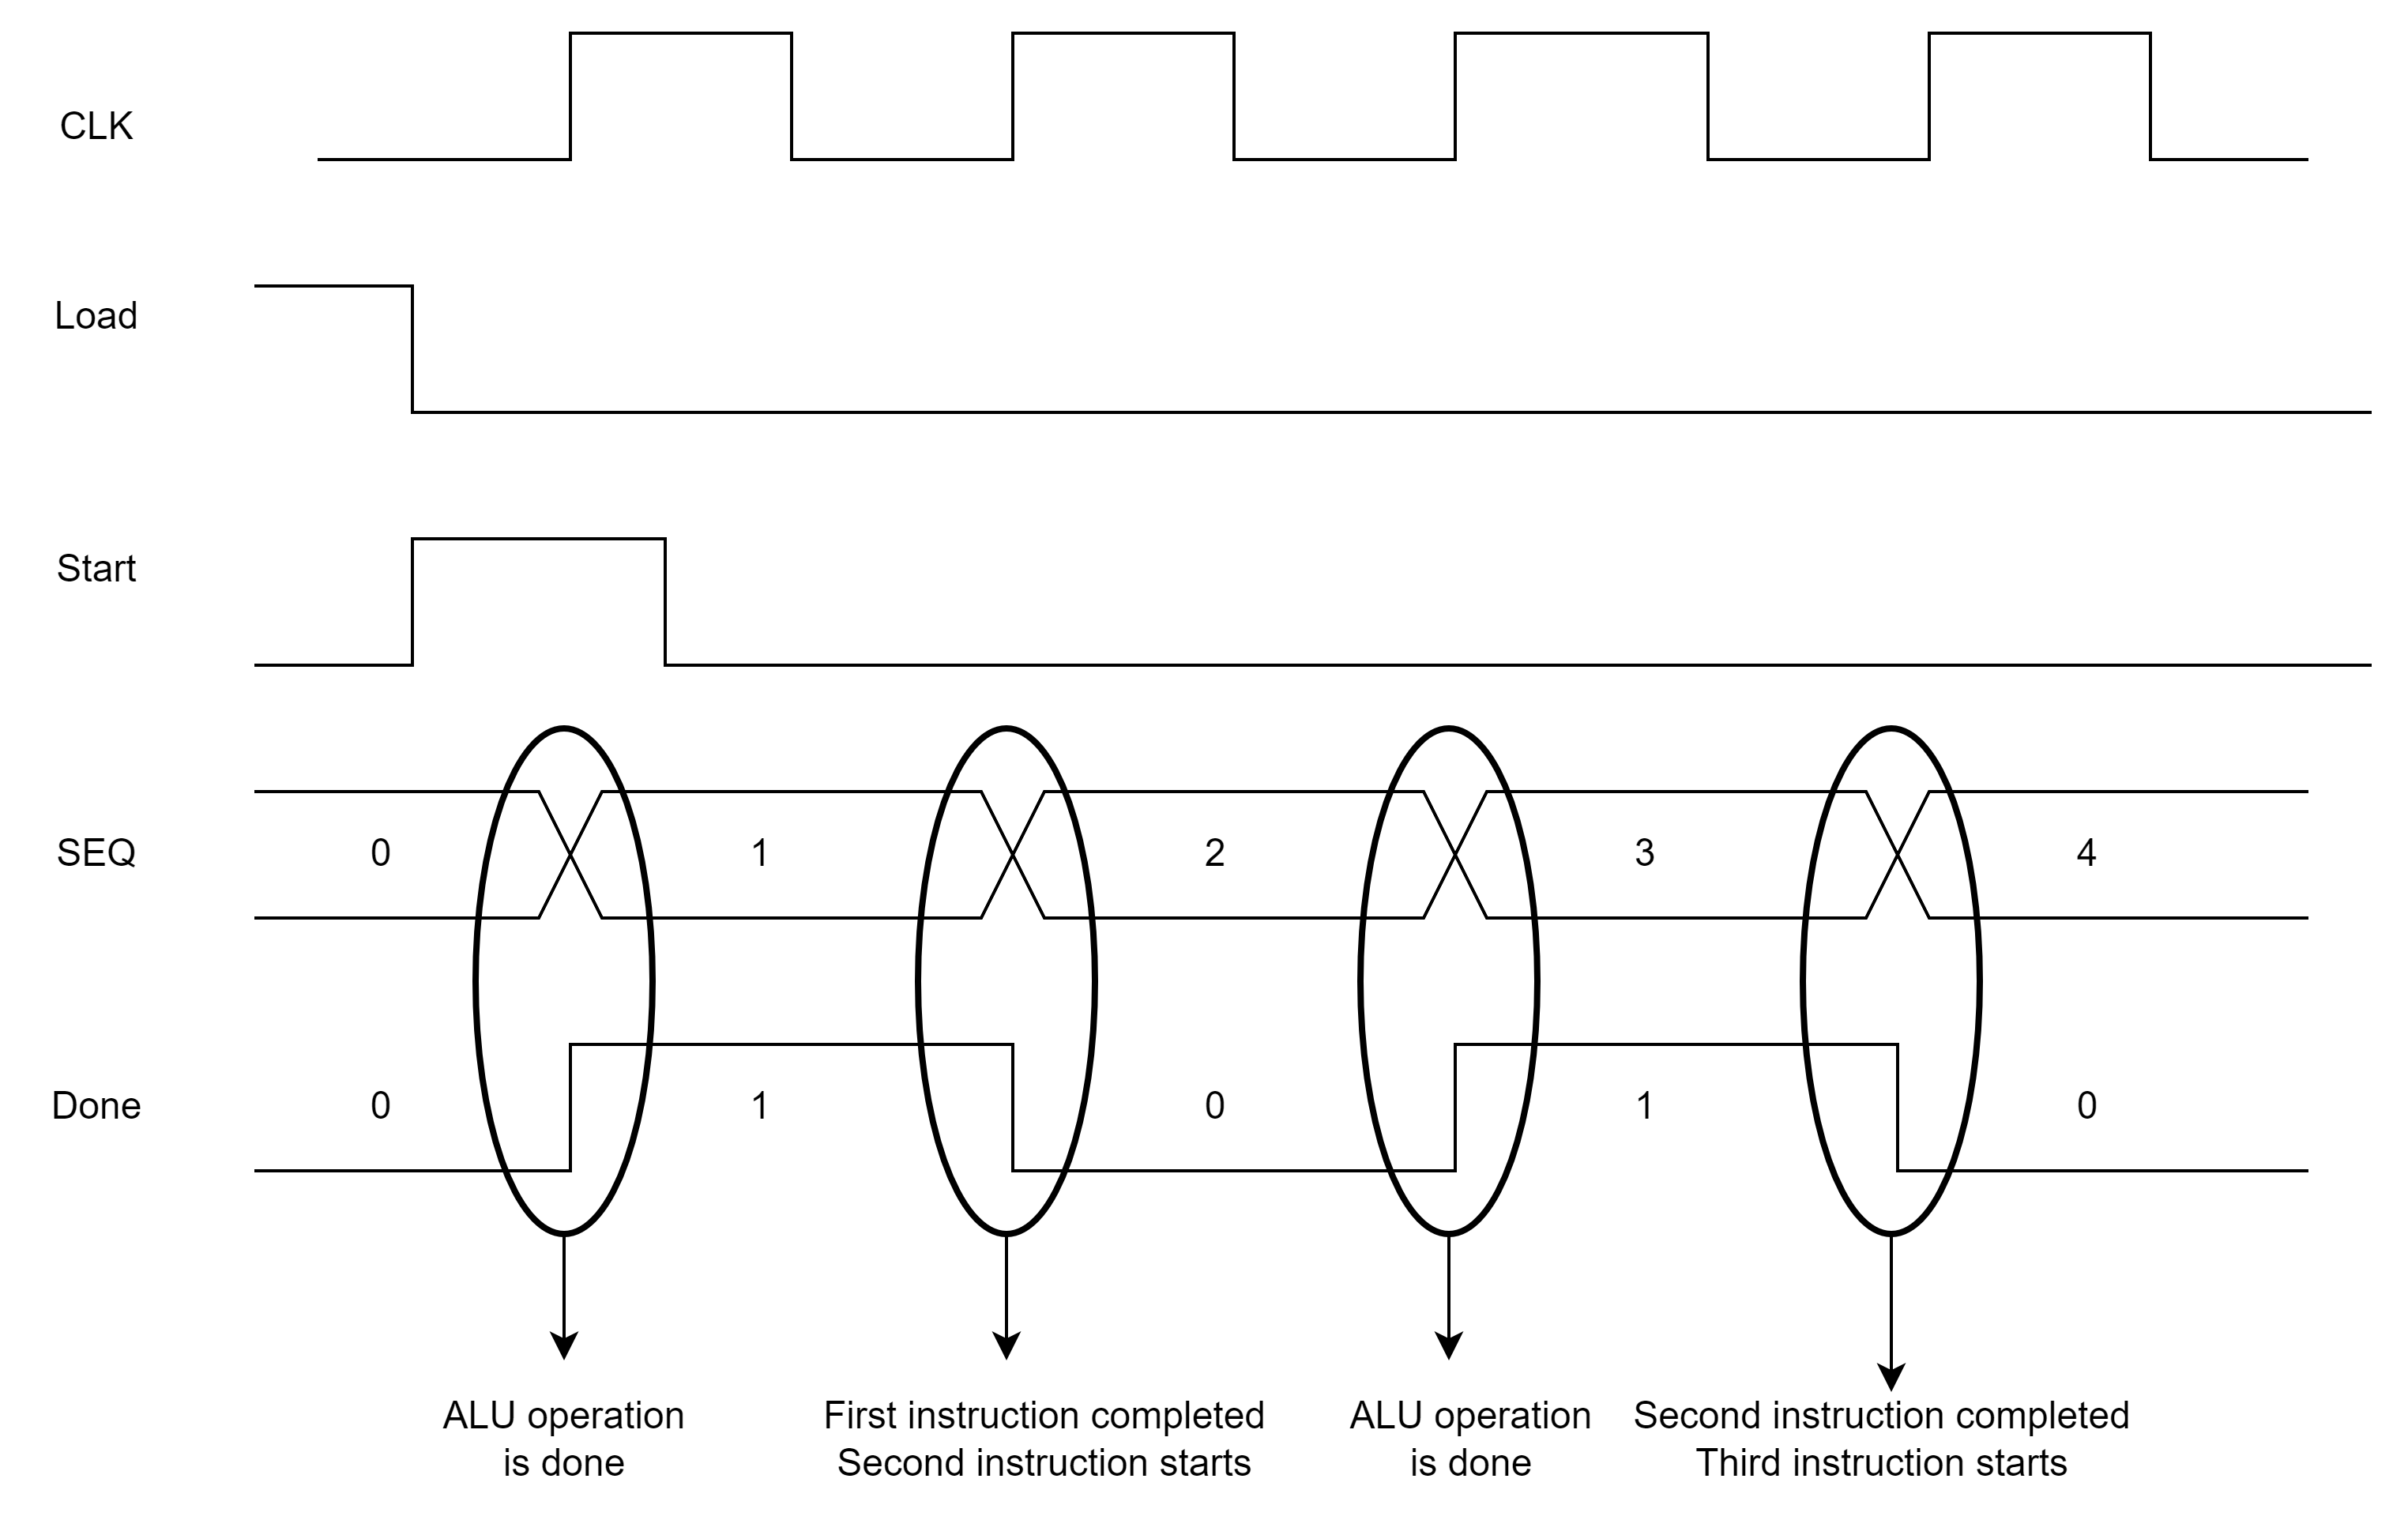
\includegraphics[scale=0.32]{timing.png}
\caption{Timing of the MCU}
\label{timing}
\end{figure}




\begin{figure}[H]
\centering
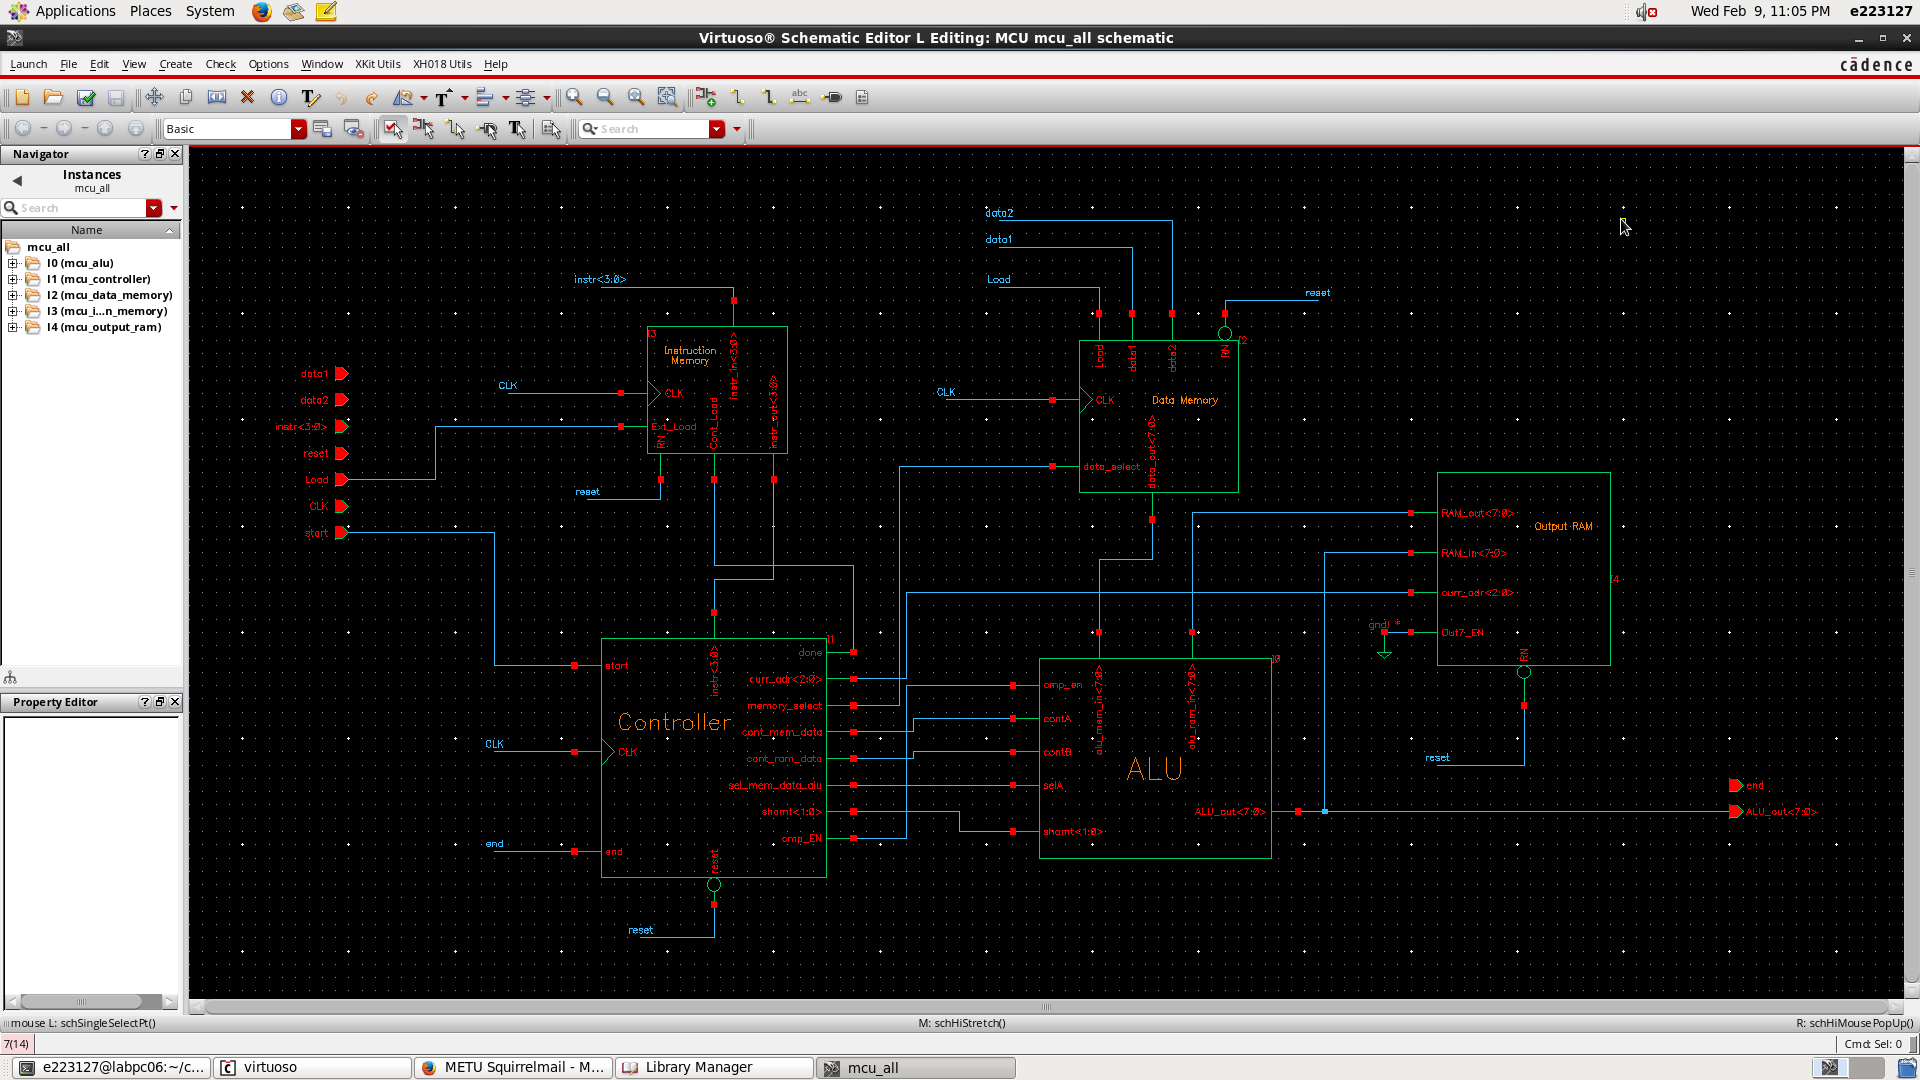
\includegraphics[scale=0.38]{all.png}
\caption{Overall Microcontroller Schematic}
\label{all}
\end{figure}

\end{landscape}
\newpage
\subsection*{Instruction Memory}
Instruction memory holds the instructions loaded to the MCU in the "Load" phase. Instructions programmed to this memory is executed during the operation. \\

Memory elements in this module is constructed using a custom register cell. This cell includes a 2$\times$1 MUX in front of a D-FF. I have avoided asynchronous elements in entire design. This is also not an exception. When the \textsl{Load} input to the cell is LOW, it preserves its state. Whenever it sees HIGH \textsl{Load}, then it loads the D-input. Schematic of the register cell can be seen in Figure \ref{reg_cell_sch}. \\

Instruction memory uses the above-mentioned cells in the cascaded form in order to shift the previously loaded instruction to the next words. There are eight 4-bit registers. It takes two different \textsl{Load} signal.One of them is from the external world. The other one comes from the controller. When the \textsl{Load} input is active, we shift the instructions closer to the output side. Note that instructions are not preserved inside the instruction memory. At the end of the operation, we do not have the instructions. As such, it is a temporary register. The internal structure can be seen in Figure \ref{instruction_mem}. \\

Zoomed version of the instruction memory in Figure \ref{instruction_zoom} shows the inputs and a few cells closer. Two \textsl{Load} signals are ORed for the load operations. It is enough to have one of them active to shift the instructions. Reset and CLK signals goes to every cell, as expected.\\

Layout of the instruction memory is drawn and can be seen in the Layouts section.

\begin{figure}[H]
\centering
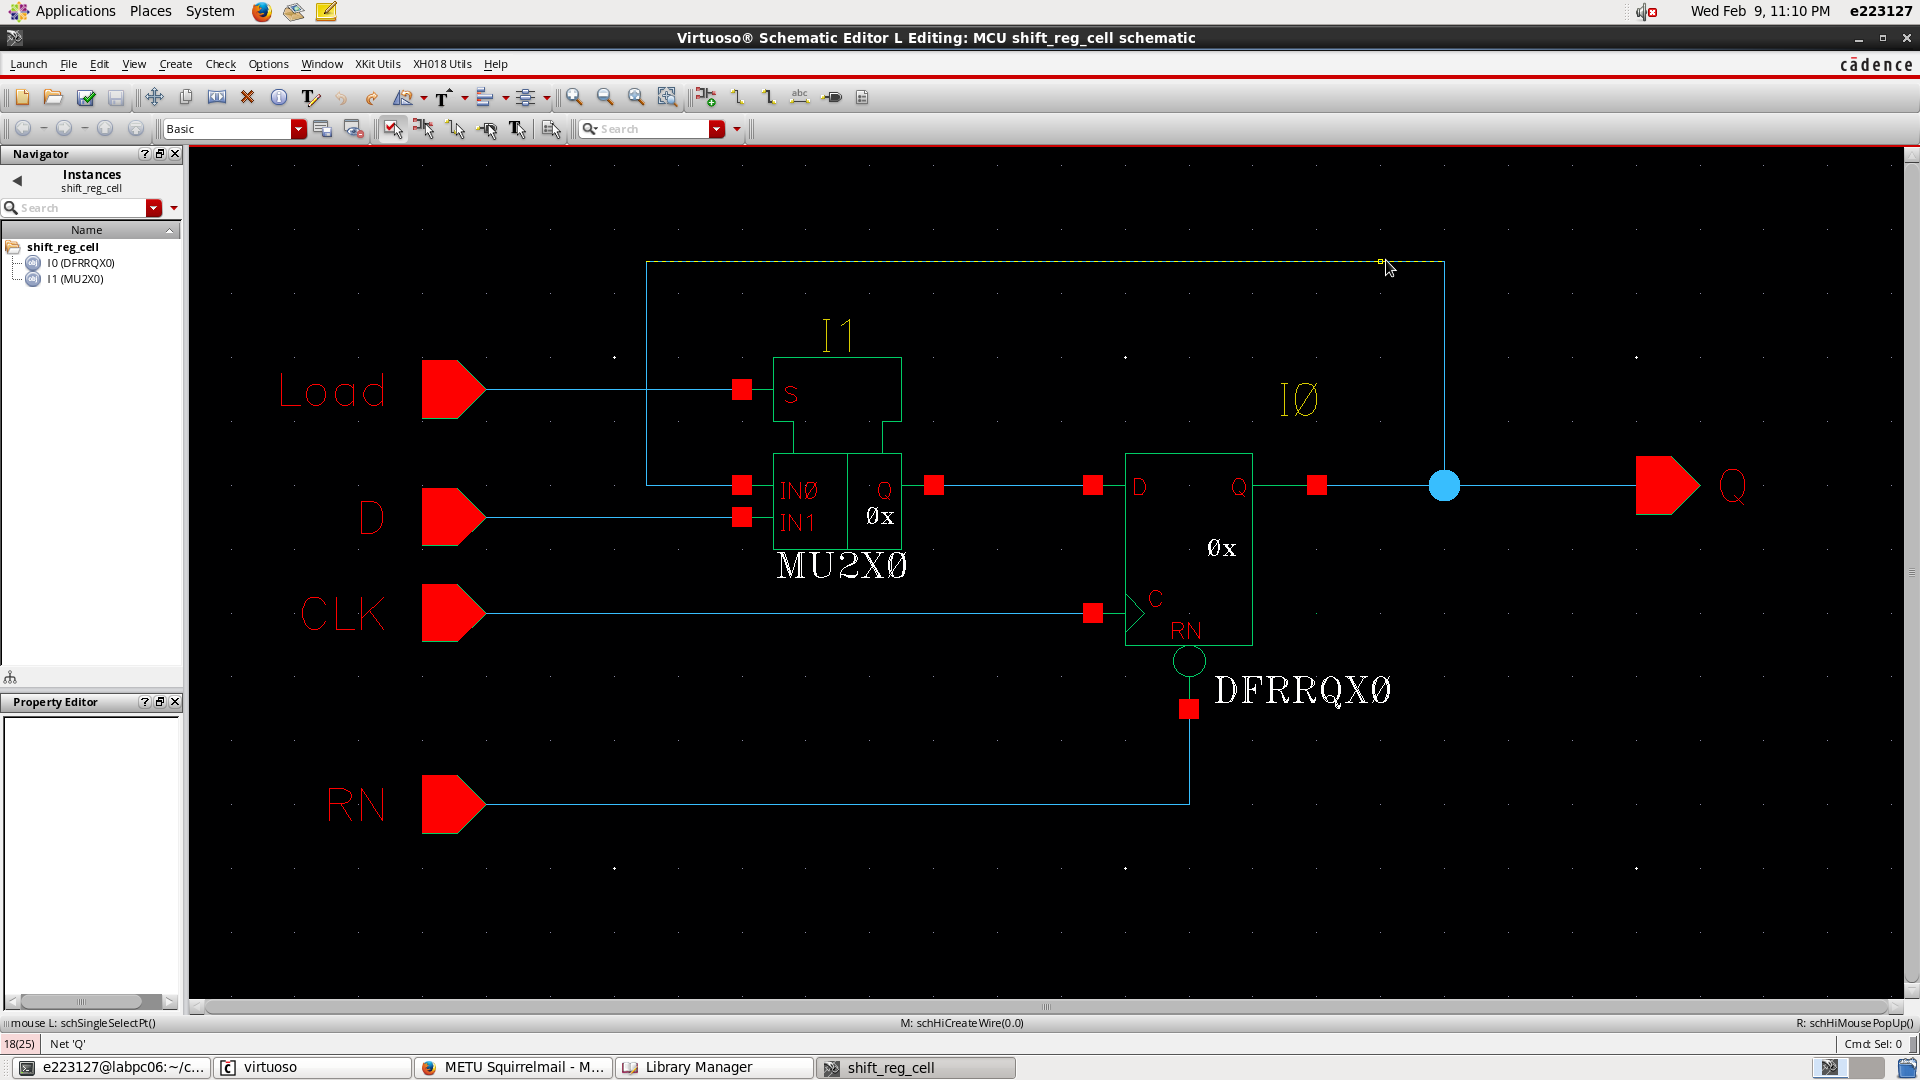
\includegraphics[scale=0.28]{reg_cell.png}
\caption{Register Cell Schematic}
\label{reg_cell_sch}
\end{figure}



\begin{landscape}
\pagestyle{empty}
\begin{figure}[H]
\centering
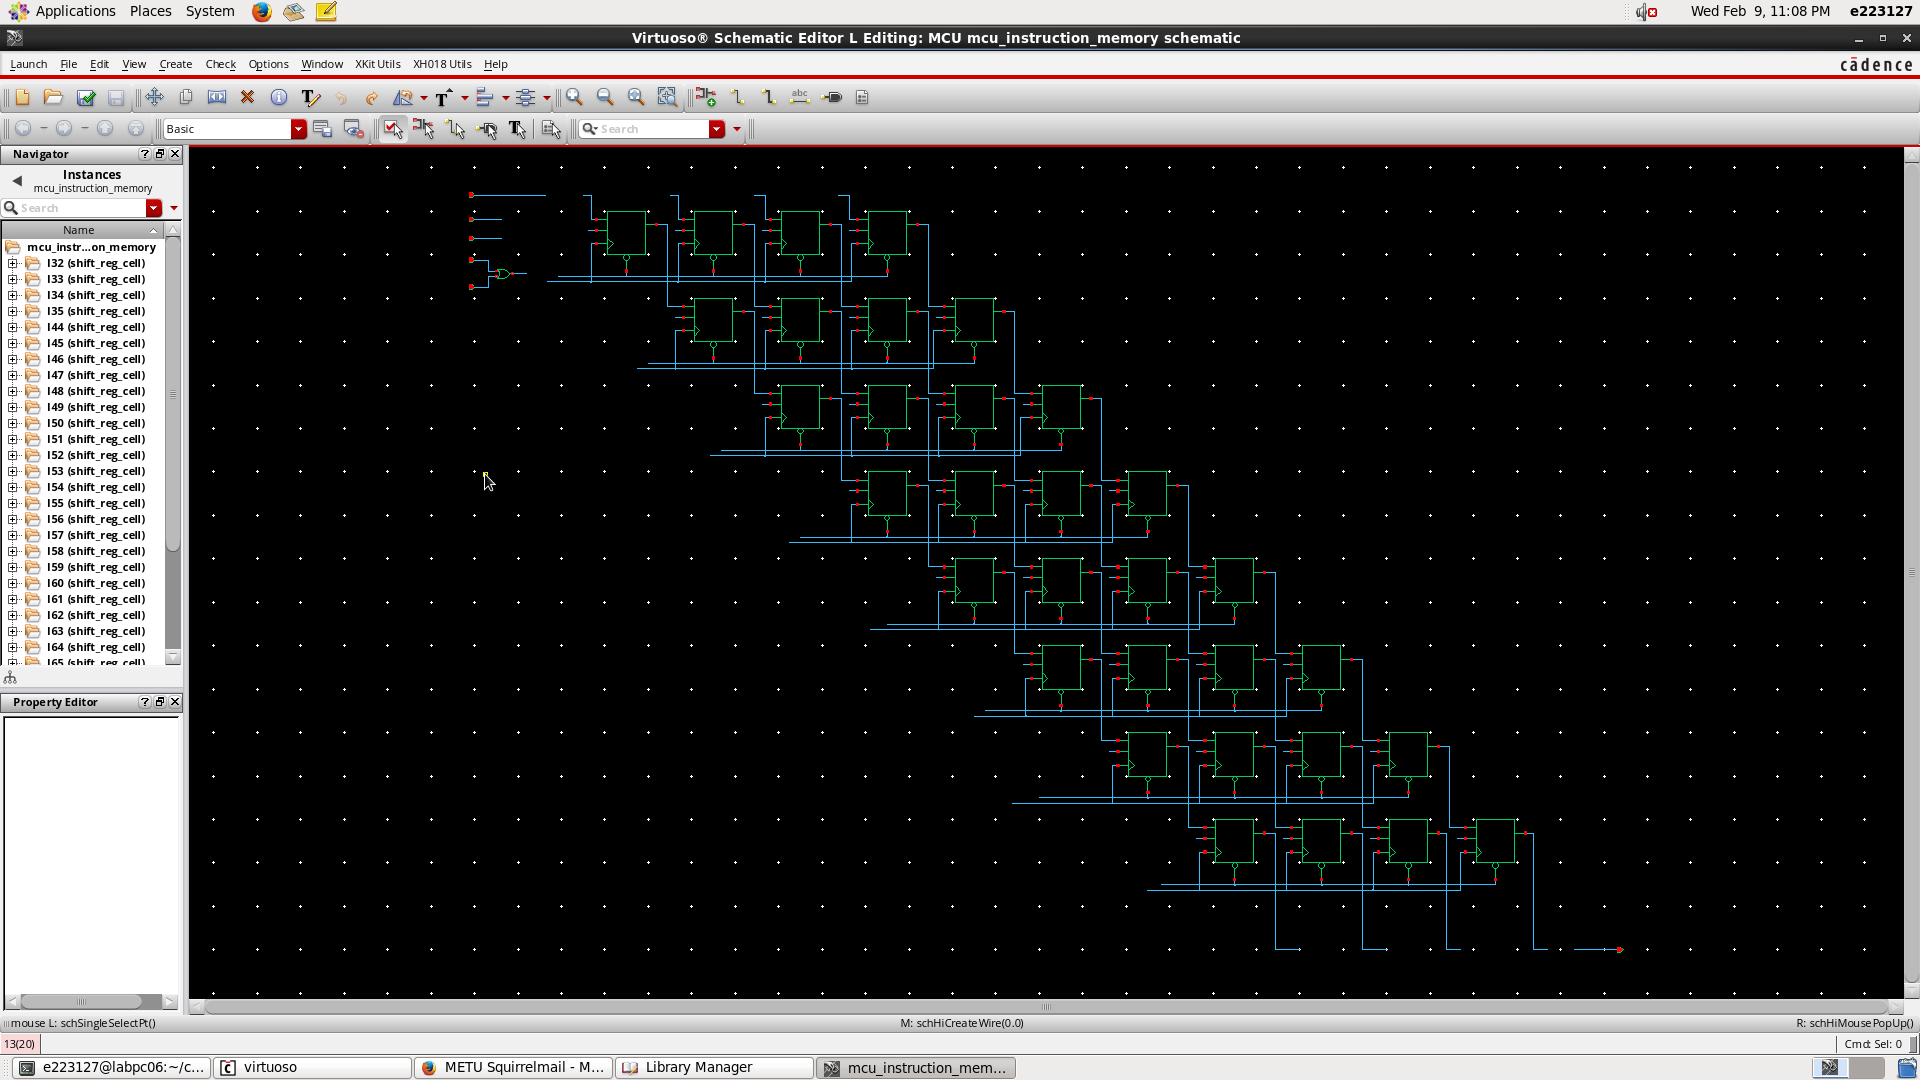
\includegraphics[scale=0.38]{instruction_mem.png}
\caption{Instruction Memory Schematic}
\label{instruction_mem}
\end{figure}


\begin{figure}[H]
\centering
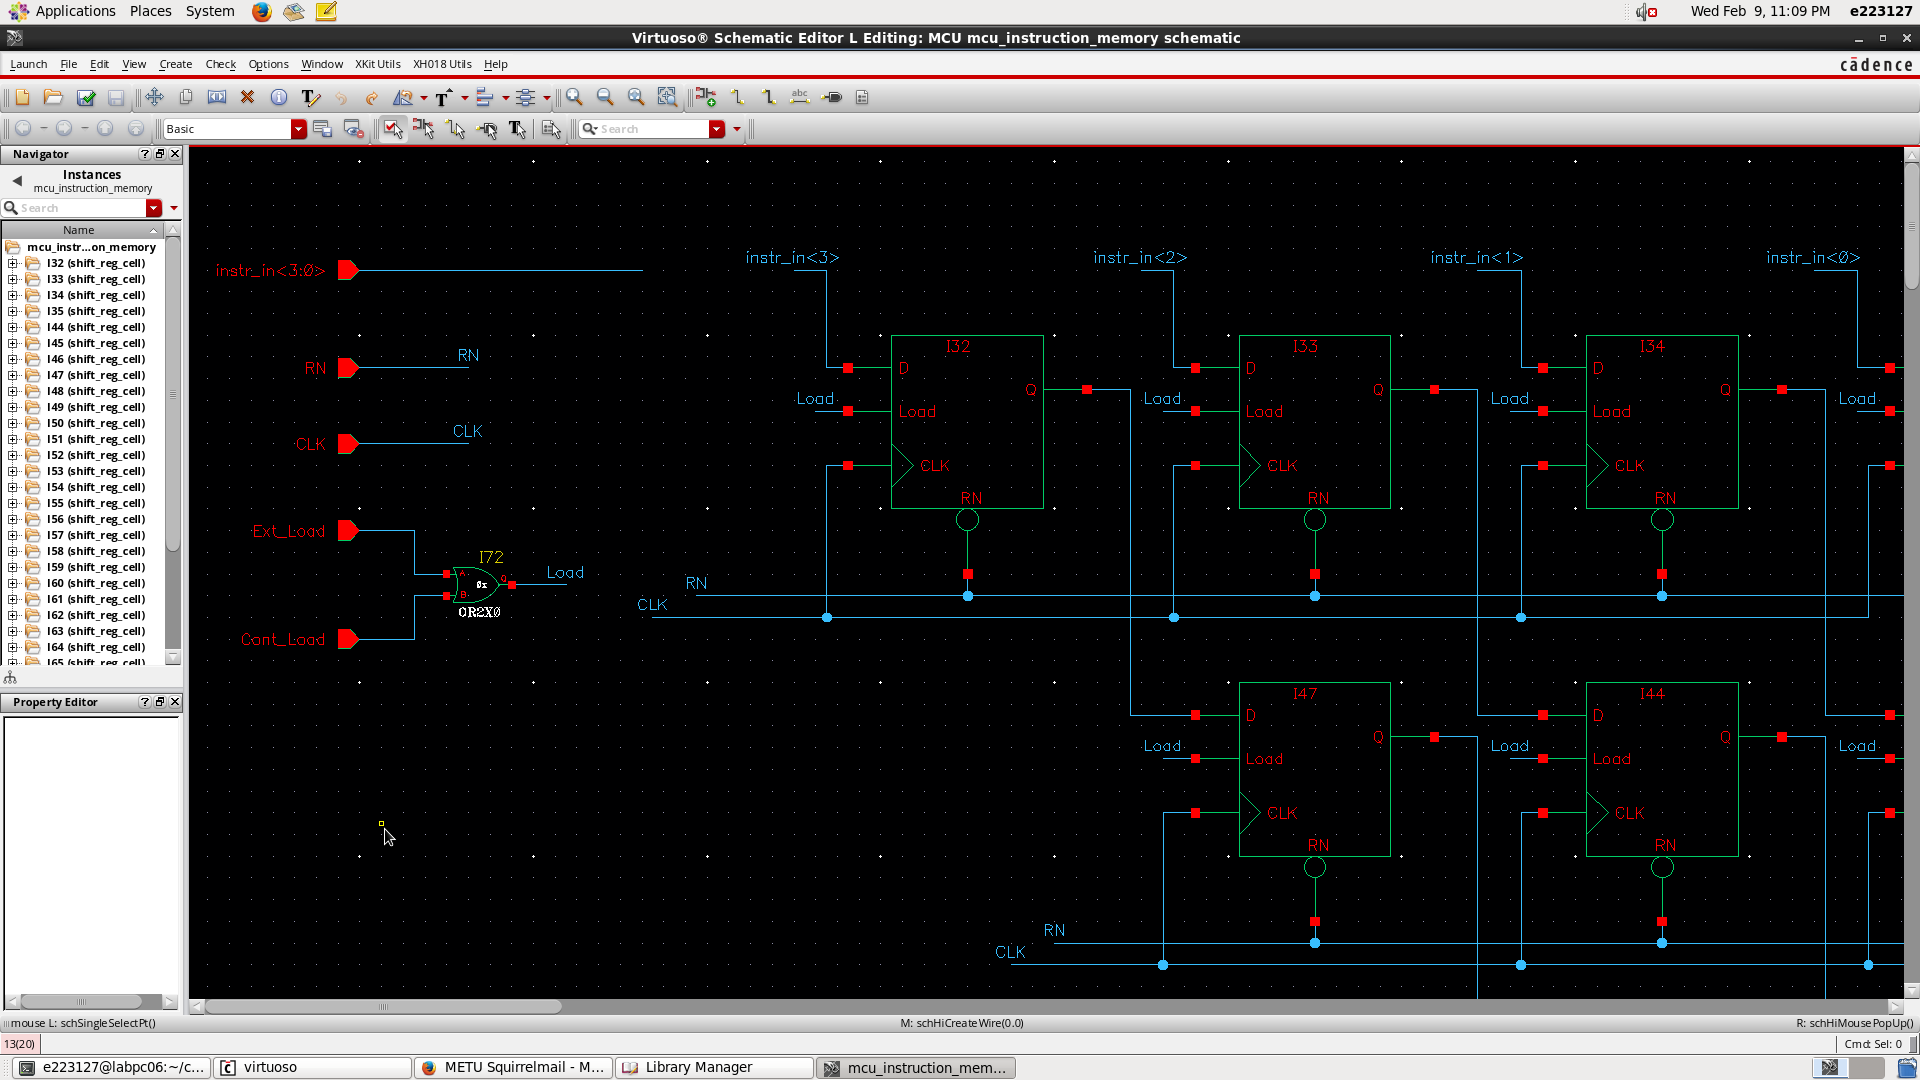
\includegraphics[scale=0.38]{instruction_zoom.png}
\caption{Instruction Memory Schematic -  Zoomed}
\label{instruction_zoom}
\end{figure}








\end{landscape}



\subsection*{Data Memory}

Data memory takes two different 8-bit number and hold them until the end of operation for processing. External \textsl{Load} signal is responsible for the loading of the data memory. There is no other \textsl{Load} signal coming to this block.\\

As explained in the architecture proposal report, in order to synchronize the external \textsl{Load} inputs, I have used 2-bit serial data to the data memory. This two bit is responsible for taking the first the second data, respectively.\\

Registers are also constructed from the cell designed for use in the MCU.(See the instruction memory section for further explanation) They are in the cascaded form. Altogether, they from 2 8-bit shift register.\\

An output MUX chooses the data to be outputted. Select signal of this MUX is coming from the controller according to the instruction.\\

Data memory schematic is shown in Figure \ref{data_mem_sch}. Layout of the data memory can be seen in the Layouts section. 

\begin{figure}[H]
\centering
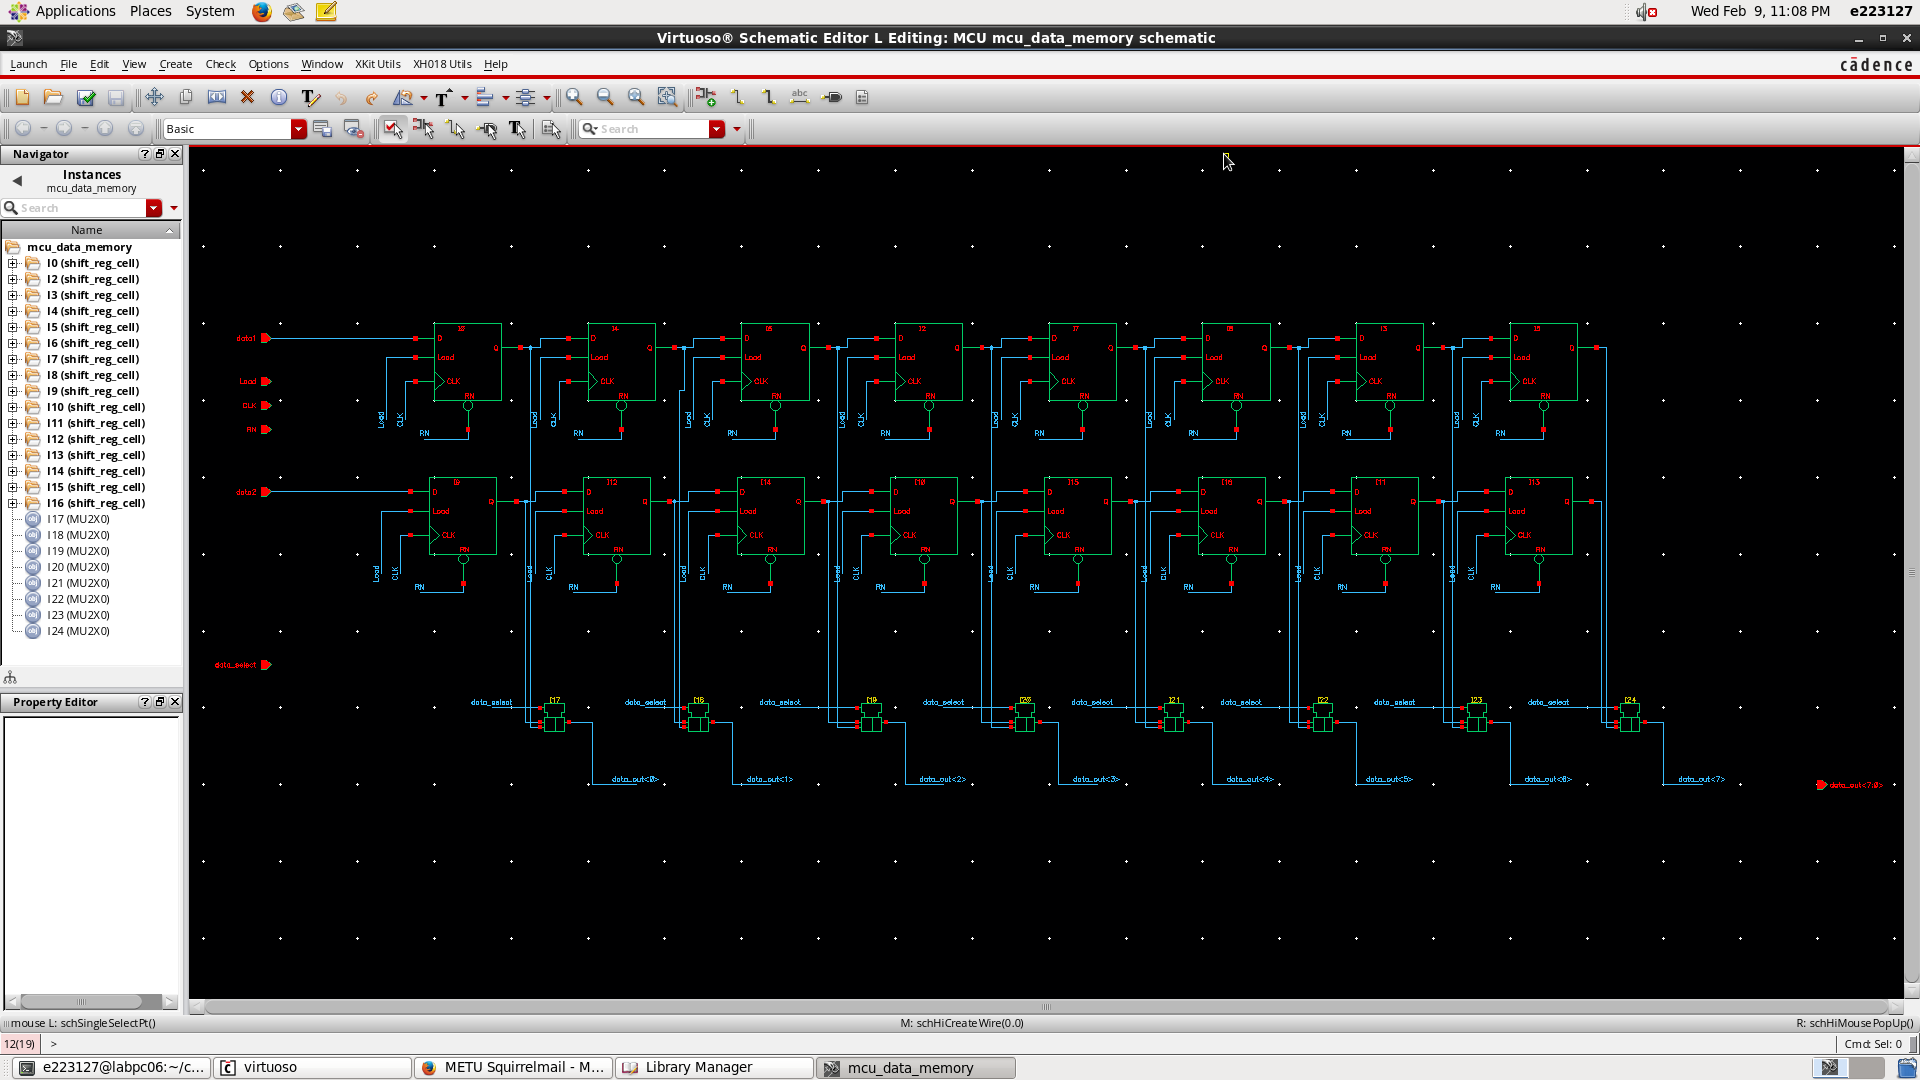
\includegraphics[scale=0.28]{data_mem.png}
\caption{Data Memory Schematic}
\label{data_mem_sch}
\end{figure}










\newpage
\subsection*{Arithmetic Logic Unit}

Arithmetic Logic Unit provides the processing power of the MCU. I designed a modular ALU structure. Each bit is processed inside an ALU Cell. Output of the ALU Cell is directly routed to the RAM. A comparator module is used inside the overall ALU structure for the comparison-based instructions.

\subsubsection*{Comparator}

\textsl{8-bit Comparator} compares the inputs and transfer result information to the ALU Cell. Comparison instructions use this information. Its output is 1 bit that shows the higher one of the inputs in modulo-2 form. Table \ref{compmode} shows the operation.\\

\begin{table}[h]
\centering
\begin{tabular}{|c|c|}
\hline 
\textbf{Case} & \textbf{Comparator Output}(\verb|cmp_result|) \\ 
\hline 
Memory Data (\verb|ALU_in_1|) $>$ RAM Data (\verb|ALU_in_2|) & 1 \\ 
\hline 
RAM Data (\verb|ALU_in_2|) $>$ Memory Data (\verb|ALU_in_1|) & 0 \\ 
\hline 
\end{tabular} 
\caption{Comparator Operation}
\label{compmode}
\end{table}

There is no need of third case because in case of equality, choice is not critical. There is no enable signal of the comparator. It works even if no comparison instructions are executed.\\

Comparator schematic can be seen in Figure \ref{comparator}. Schematic is constructed using the following logical operation.\\

Let 
\begin{align*}
x_i = A \odot B = (A\cdot B + \overline{A}\cdot \overline{B})
\end{align*}
Then,

\begin{align*}
(A>B) = &{A_7}\overline{B_7} + x_7 {A_6}\overline{B_6} + x_7 x_6 {A_5}\overline{B_5} + x_7 x_6 x_5 {A_4}\overline{B_4} + x_7 x_6 x_5 x_4 {A_3}\overline{B_3} \\
 &+ x_7 x_6 x_5 x_4 x_3 {A_2}\overline{B_2} + x_7 x_6 x_5 x_4 x_3 x_2 {A_1}\overline{B_1} + x_7 x_6 x_5 x_4 x_3 x_2 x_1 {A_0}\overline{B_0}
\end{align*}





\subsubsection*{ALU Cell}

ALU Cell is a single bit processor which is capable of doing the following operations.
\begin{itemize}
\item Set
\item Reset 
\item Load \verb|ALU_in_1|
\item Load \verb|ALU_in_2|
\item Shift Left \verb|ALU_in_2|
\item Shift Right \verb|ALU_in_2|
\item Compare \verb|ALU_in_1| and \verb|ALU_in_2|, write the higher one
\item Add \verb|ALU_in_1| + \verb|ALU_in_2|
\item Subtract \verb|ALU_in_1| - \verb|ALU_in_2|
\item Subtract \verb|ALU_in_2| - \verb|ALU_in_1|
\end{itemize}


All of the above operations are done via the following ALU cell structure in Figure \ref{alu_cell_conceptual}. To briefly explain the functionality of every component

\begin{itemize}
\item Full Adder(FA) can add, subtract and transfer the inputs with the correct configurations.
\item XORs(exclusive OR) in front of the FA inputs is used to define the subtraction operation. Inputs we want to subtract is XORed with 1.
\item AND gate in series with the memory input is used for the suppress the inputs from data memory. This is used for transfer operations.
\item 4$\times$1 MUX in the RAM side is used as a combinational shifter(also called Barrel Shifter). Shift left, shift right operations are done at this point. Remaining components are configured to load condition for the shift operations. Operation of the Barrel shifter can be summarized as in Table \ref{shamt}. 0 input is used for the suppression. \textsl{shamt} inputs is dictated by the controller.

\begin{table}[h]
\centering
\begin{tabular}{|c|c|}
\hline 
\textbf{shamt[1:0]} & \textbf{Operation} \\ 
\hline 
00 & No shift \\ 
\hline 
01 & Output Logic 0(used for suppression) \\ 
\hline 
10 & Shift Left \\ 
\hline 
10 & Shift Right \\ 
\hline 
\end{tabular} 
\caption{Shift Mode Operations}
\label{shamt}
\end{table}

\item Comparison based instructions use the compare-enable input from the controller. When this input is active, we look at the comparator output. If it is HIGH, we load the data memory input, if it is LOW, we load the RAM input(see the comparator section above).
\end{itemize}

General ALU cell operation can be summarized in the Table \ref{alu_modes}.


\begin{table}
\centering
\begin{tabular}{|c|c|c|c|c|c|c|}
\hline 
\textbf{Operation} & \textbf{sel-mem} & \textbf{cont-mem} & \textbf{cont-ram} & \textbf{shamt[1]} & \textbf{shamt[0]} & \textbf{cmp-en} \\ 
\hline 
Set & 0 & 0 & 1 & 0 & 1 & 0 \\ 
\hline 
Reset & 0 & 0 & 0 & 0 & 1 & 0 \\ 
\hline 
Load-mem & 1 & 0 & 0 & 0 & 1 & 0 \\ 
\hline 
Load-ram & 0 & 0 & 0 & 0 & 0 & 0 \\ 
\hline 
Add & 1 & 0 & 0 & 0 & 0 & 0 \\ 
\hline 
Subtract mem-ram & 1 & 0 & 1 & 0 & 0 & 0 \\ 
\hline 
Subtract ram-mem & 1 & 1 & 0 & 0 & 0 & 0 \\ 
\hline 
Compared Load & cmp-result & 0 & 0 & 0 & cmp-result & 1 \\ 
\hline 
Shift Left ram & 0 & 0 & 0 & 1 & 0 & 0 \\ 
\hline 
Shift Right ram & 0 & 0 & 0 & 1 & 1 & 0 \\ 
\hline 
\end{tabular} 
\caption{ALU Cell Operations and Inputs}
\label{alu_modes}
\end{table}


\begin{figure}[H]
\centering
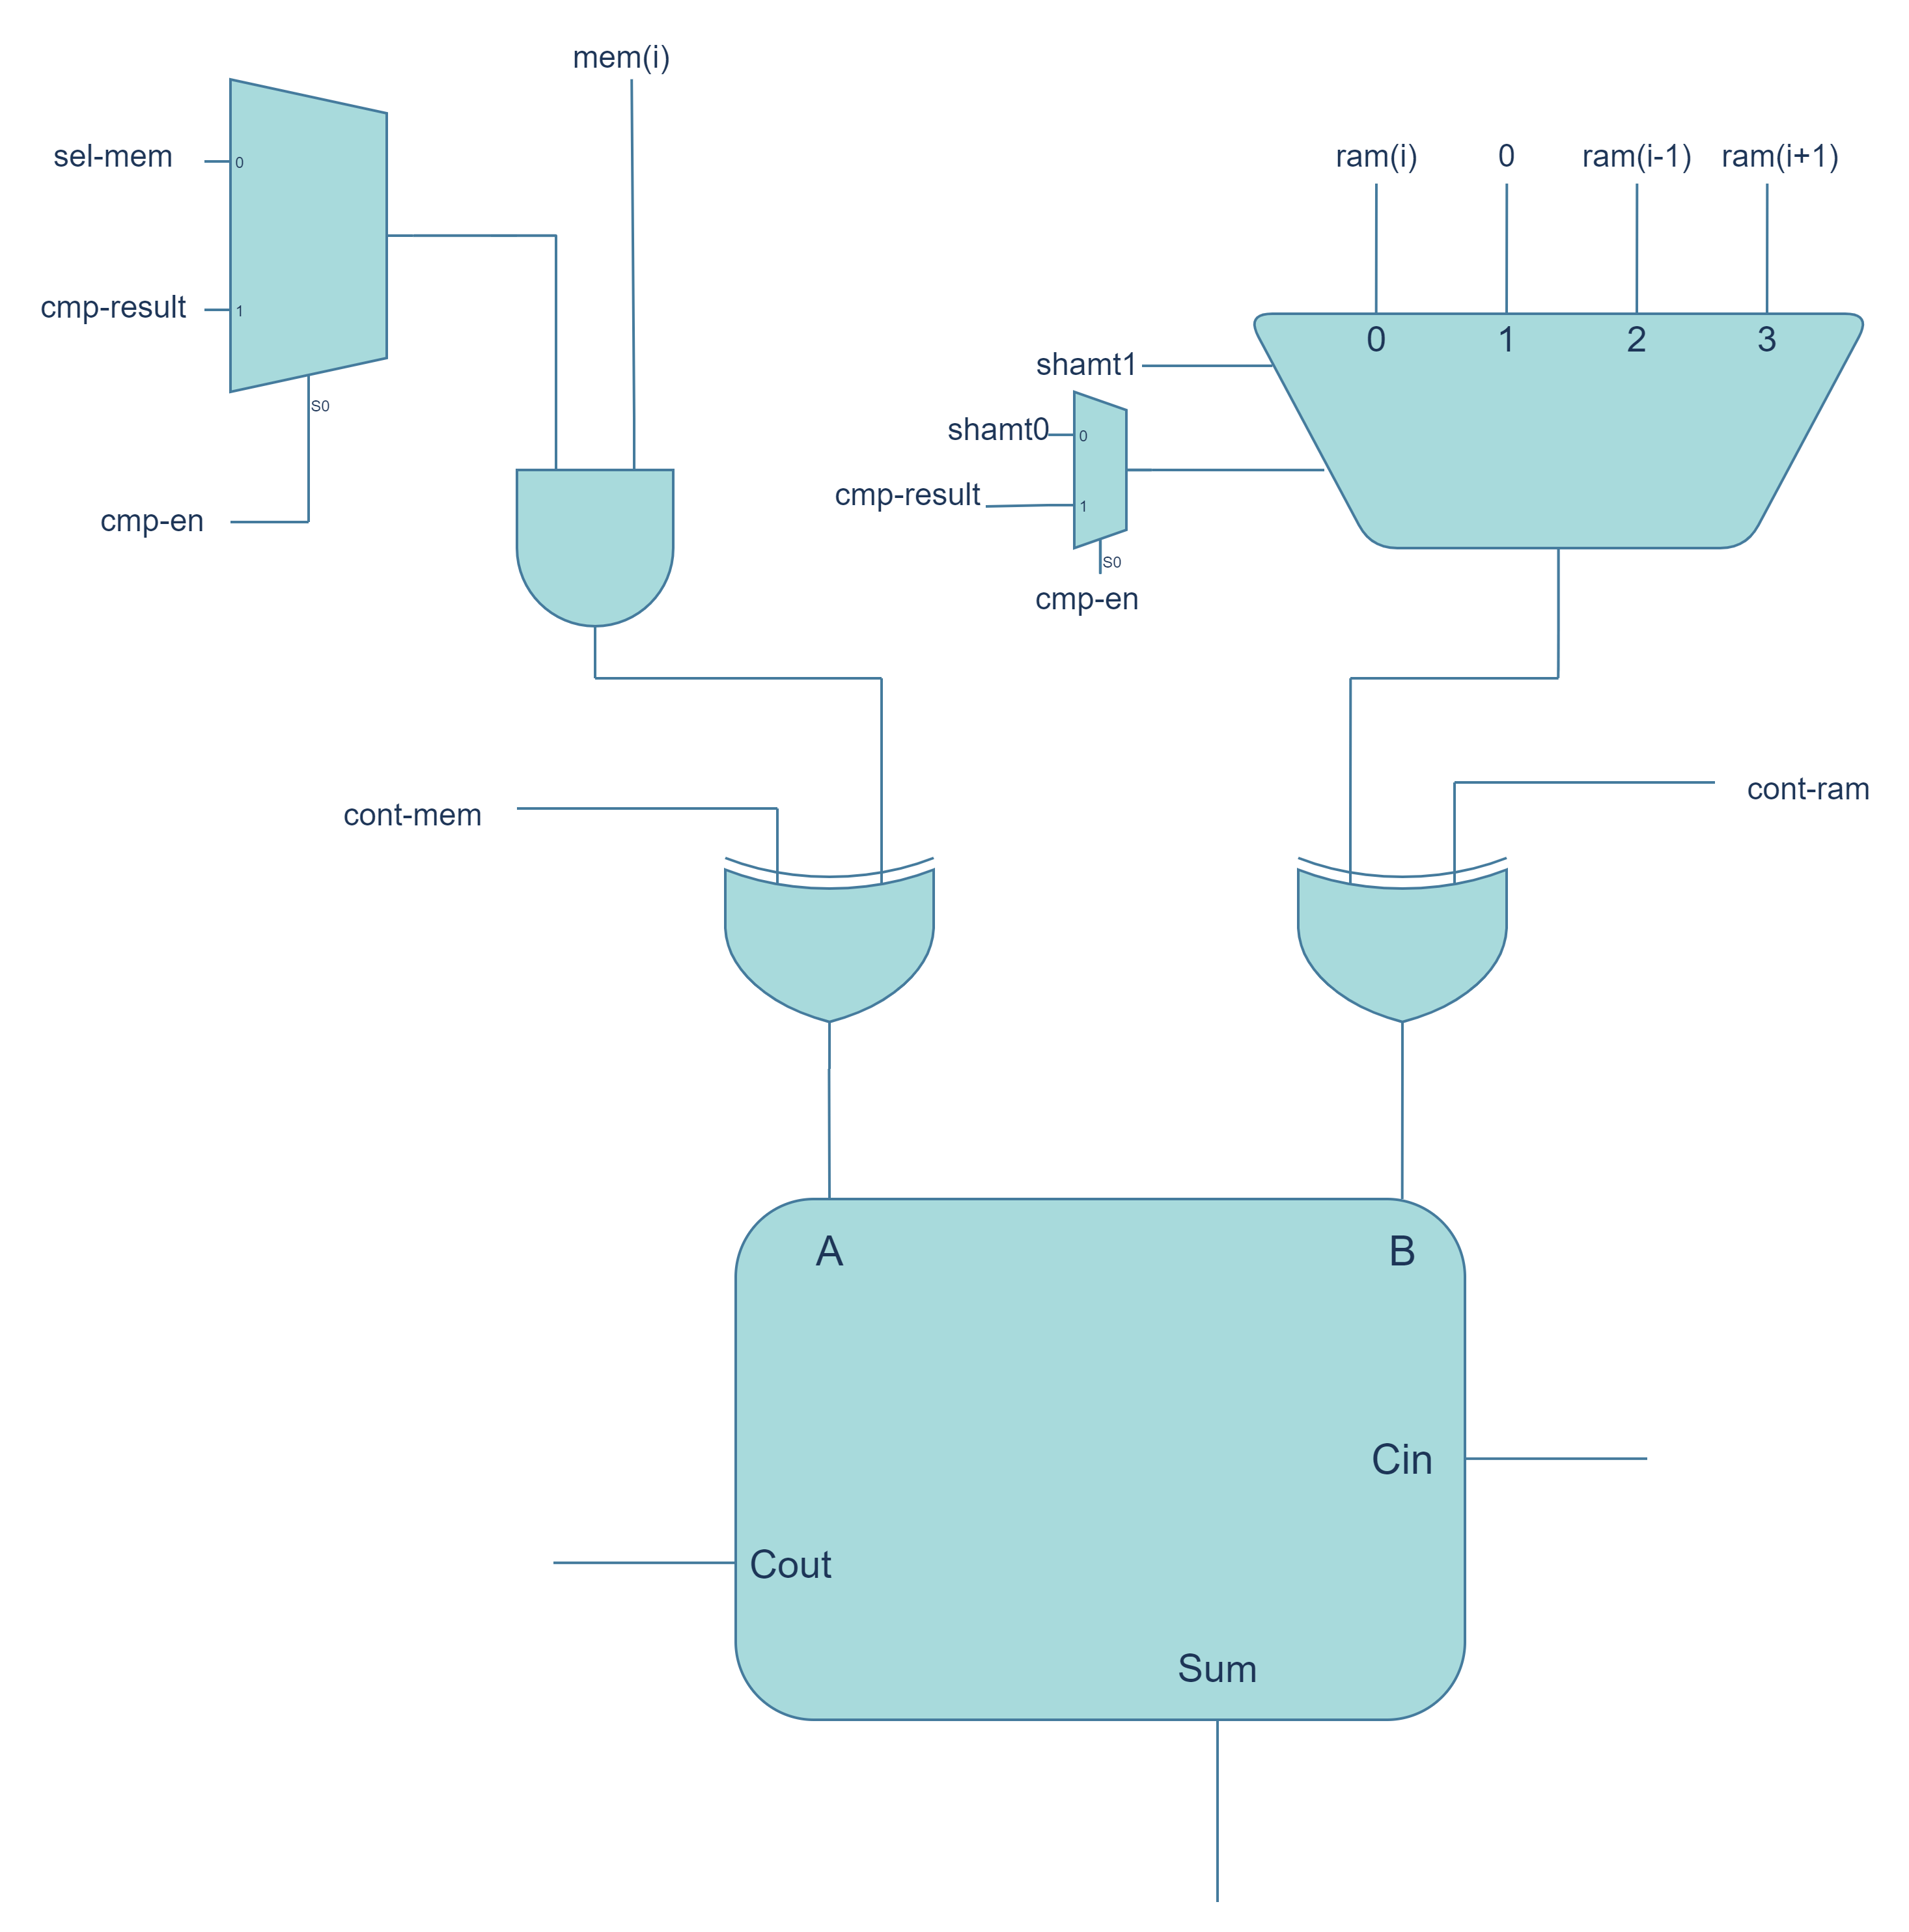
\includegraphics[scale=0.22]{alu_cell_conceptual.png}
\caption{ALU Cell Conceptual Drawing}
\label{alu_cell_conceptual}
\end{figure}


Schematic of the ALU Cell is provided in Figure \ref{alu_cell}.\\

ALU structure use 8 of the ALU cells and a comparator. Its schematic can be seen in Figure \ref{alu_sch}.

\begin{landscape}

\begin{figure}[H]
\centering
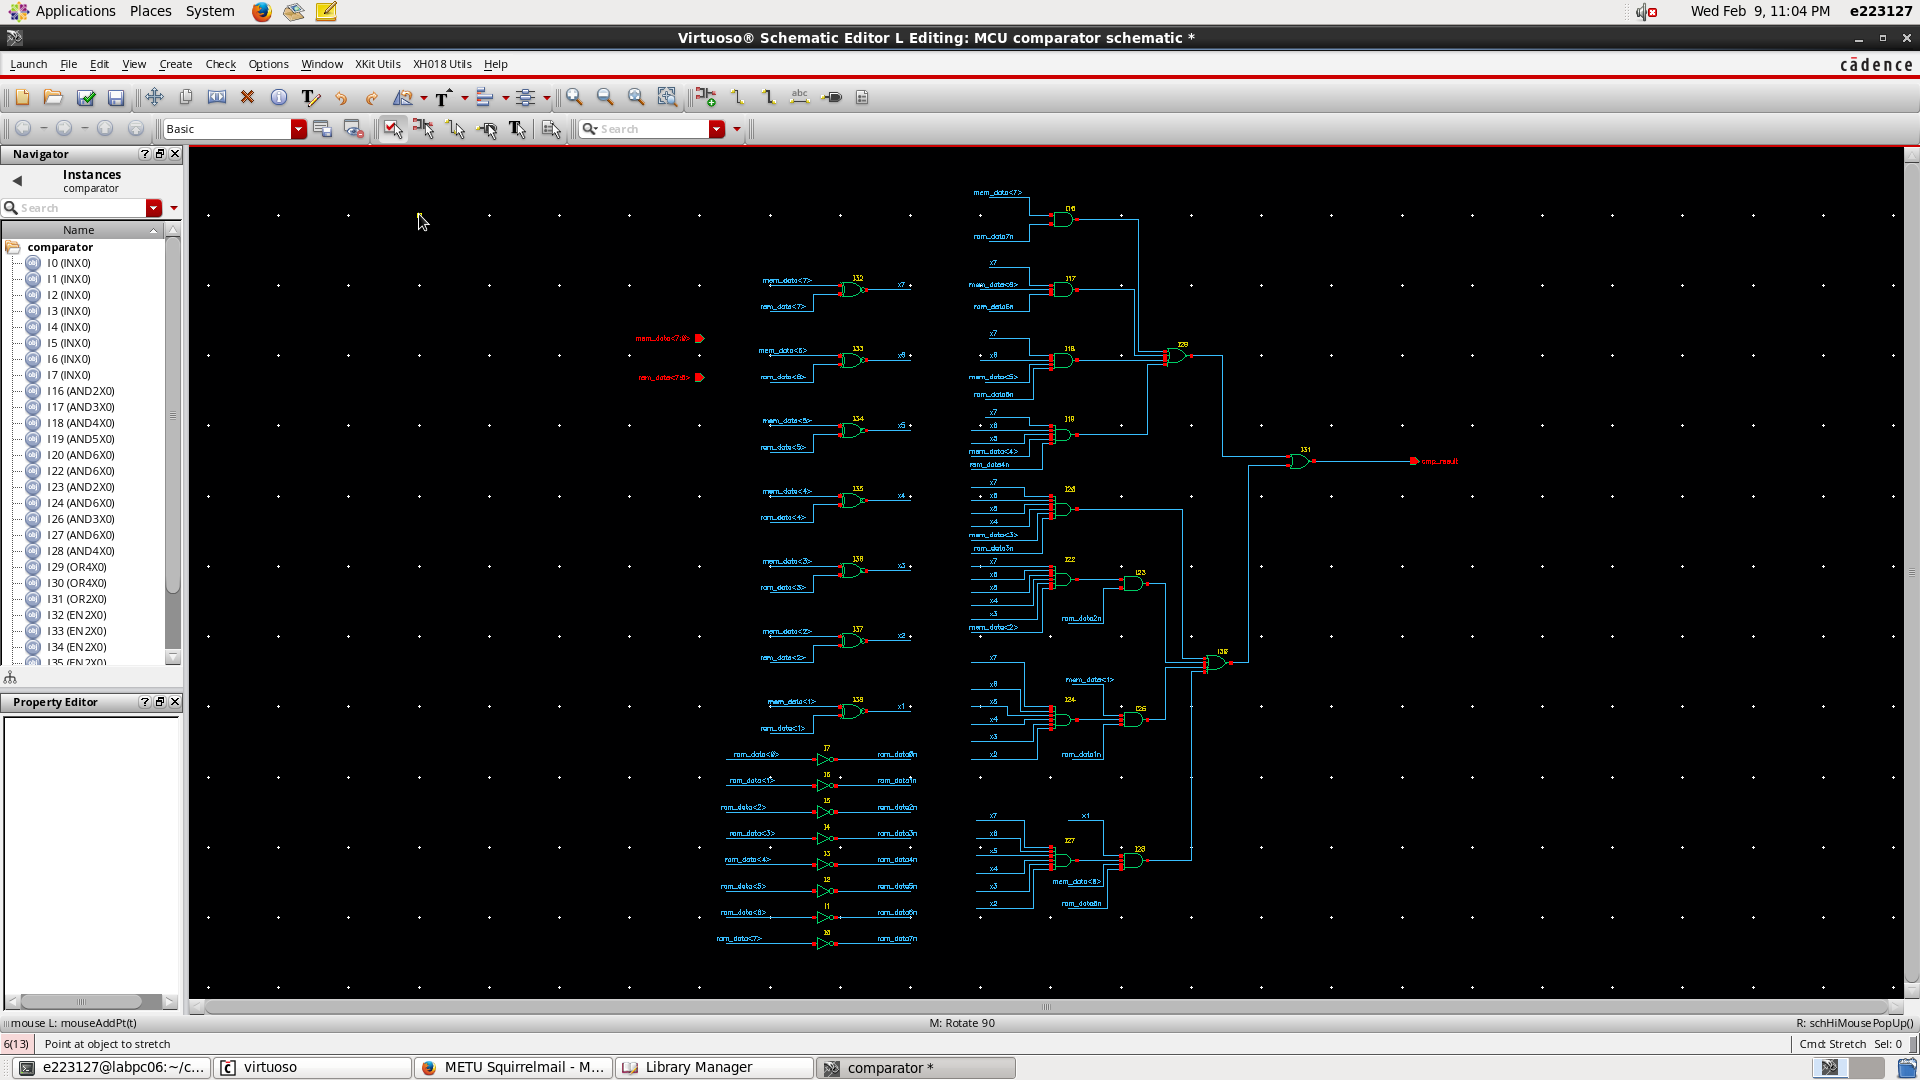
\includegraphics[scale=0.38]{comparator.png}
\caption{Comparator Schematic}
\label{comparator}
\end{figure}


\pagestyle{empty}
\begin{figure}[H]
\centering
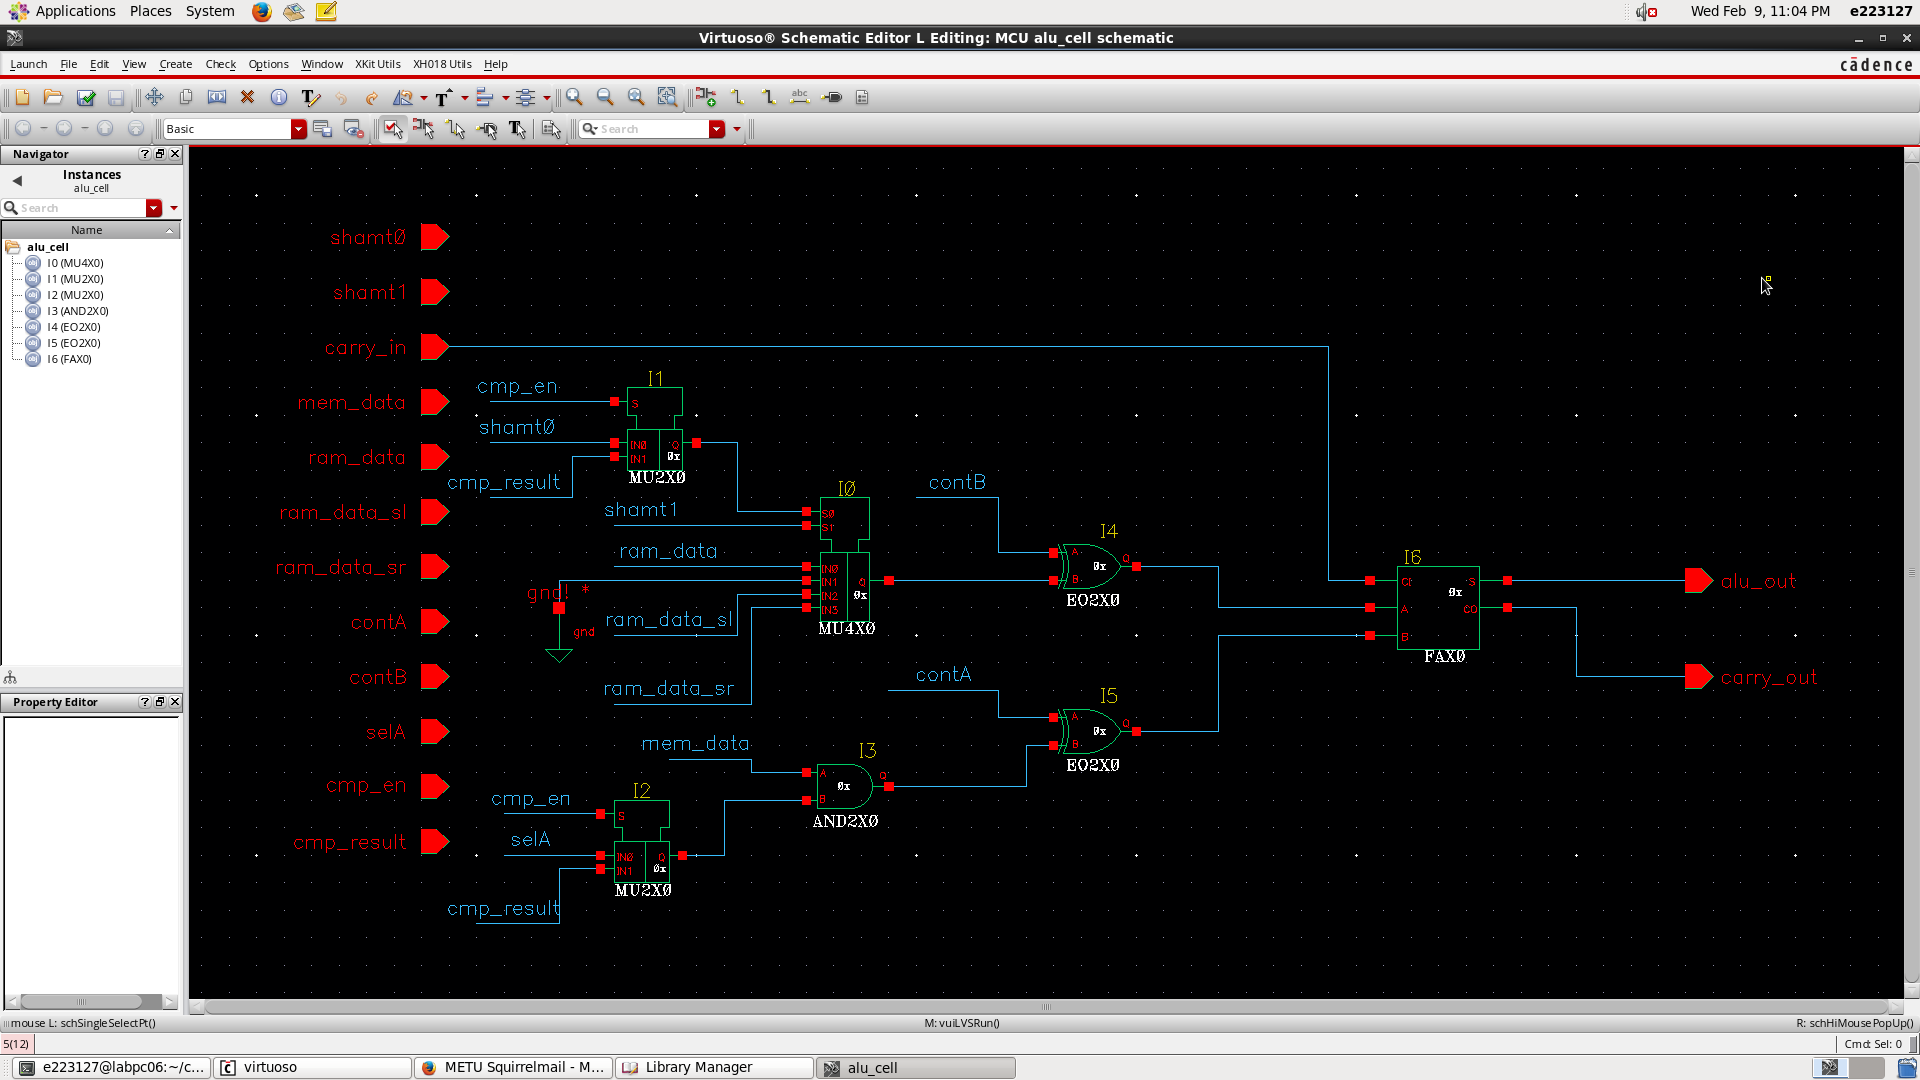
\includegraphics[scale=0.38]{alu_cell.png}
\caption{ALU Cell Schematic}
\label{alu_cell}
\end{figure}


\begin{figure}[H]
\centering
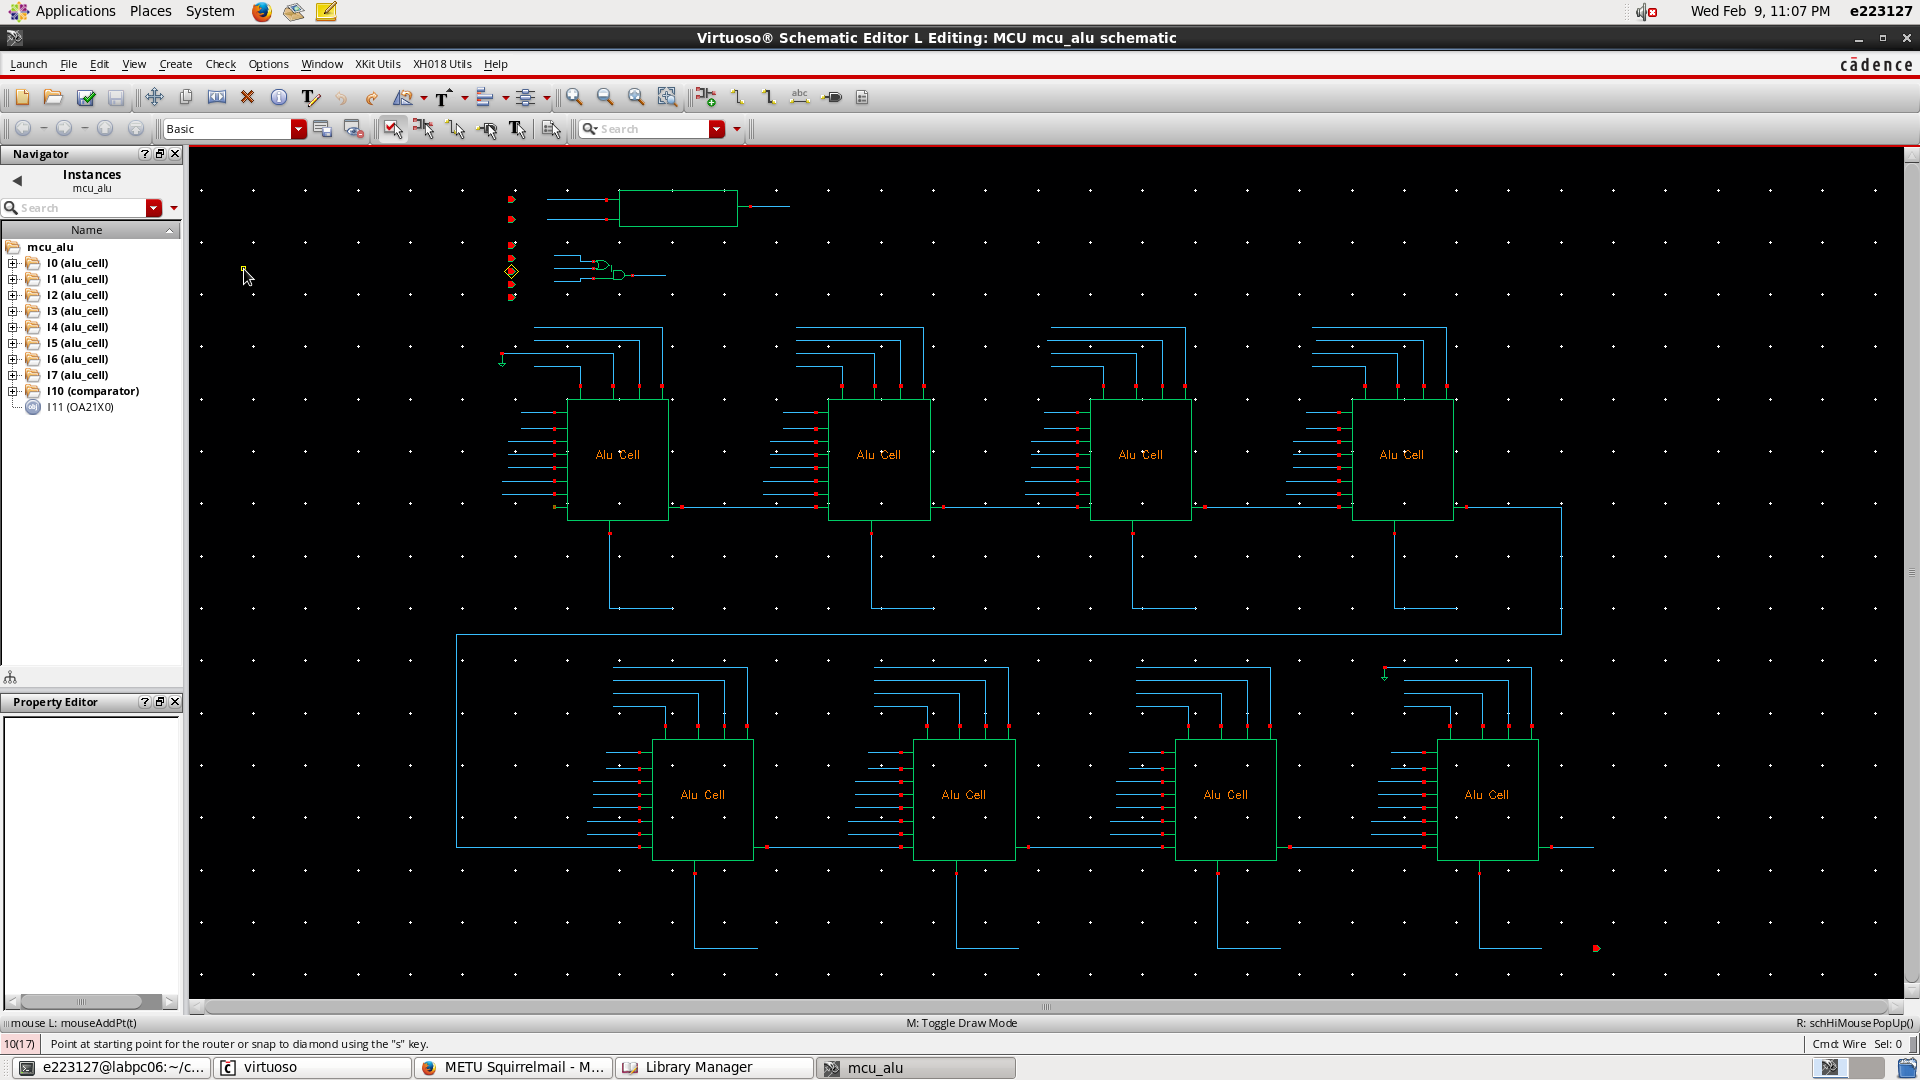
\includegraphics[scale=0.38]{alu.png}
\caption{Arithmetic Logic Unit Schematic}
\label{alu_sch}
\end{figure}


\end{landscape}



\subsection*{Controller}


Controller is the heart of the microcontroller. Figure \ref{controller} shows the schematic of the controller.\\

Sequence counter schematic can be seen in Figure \ref{seq_cnt}. It is used to trace the timing. It is explained in detail in the Timing section in the beginning. Its count input is enabled by a D-FF in the controller. This D-FF looks for the \textsl{Start} signal and \textsl{End} instruction. When the operations starts it enables the sequence counter to count. End instruction ends this mode.\\

Control logic takes the current instruction and produces the control signals for the data memory and ALU. There are 8 control signals produced by the controller. These are as follows together with their purpose.
\begin{itemize}
\item sel-mem-data-alu : controls the suppression of the memory data in ALU.
\item cont-mem-data : controls the subtraction of memory data in the ALU. 
\item cont-ram-data : controls the subtraction of RAM data in the ALU.
\item shamt[1:0] : controls the shift amount of the RAM data, also accounts for the suppression of it.
\item memory-select : controls the data  memory output.
\item cmp-en : controls the comparison enable.
\item Done : controls the instruction memory load operation. It is produced by sequence counter. It is the LSB bit of SC.
\end{itemize} 

Outputs of the controller is defined in Table \ref{signals}. I will not include the Karnaugh maps I used to optimize the logical operations. Below, you can find the result of this minimization. For simplicity, just the numbers are used instead of writing $instr<3>$, $instr<2>$ etc.

\begin{align*}
sel\_ mem\_ data\_ alu &= 2 \oplus 3 + \overline{1} \cdot 2 \\
cont\_ mem\_ data &= 0 \cdot \overline{1} \cdot 2 \cdot \overline{3} + \overline{0} \cdot 1 \cdot \overline{2} \cdot 3 \\
cont\_ ram\_ data &= \overline{0} \cdot 1 \cdot 2 \cdot \overline{3} + 0 \cdot 1 \cdot \overline{2} \cdot 3 + 0 \cdot \overline{1} \cdot \overline{2} \cdot \overline{3} \\
shamt[1] &= 1 \cdot \overline{2} \cdot \overline{3} \\
shamt[0] &= 0 \cdot \overline{2} \cdot \overline{3} + \overline{0} \cdot \overline{1} \cdot 2 \cdot \overline{3} + \overline{0} \cdot 1 \cdot 2 \cdot 3 + 0 \cdot \overline{1} \cdot \overline{2} \\
memory\_select &= \overline{0} \cdot \overline{1} \cdot \overline{2} + \overline{3} \\
cmp\_en &= \overline{0} \cdot \overline{1} \cdot \overline{2} \cdot 3 + 0 \cdot \overline{1} \cdot 2 \cdot 3 \\
\end{align*}

Above logical decision mechanisms are implemented in the controller schematics with the primitive gates. End output is controlled as

\begin{align*}
end = 1 \cdot 2 \cdot 3 \cdot Done
\end{align*}



\begin{landscape}
\pagestyle{empty}


\begin{table}[h]
\centering
\begin{tabular}{|c|c|c|c|c|c|c|c|}
\hline 
\textbf{Instruction[3:0]} & \textbf{sel-mem-data-alu} & \textbf{cont-mem-data} & \textbf{cont-ram-data} & \textbf{shamt[1]} & \textbf{shamt[0]} & \textbf{memory-select} & \textbf{cmp-en} \\ 
\hline 
0000 & 0 & 0 & 0 & 0 & 0 & X & 0 \\ 
\hline 
0001 & 0 & 0 & 1 & 0 & 1 & X & 0 \\ 
\hline 
0010 & 0 & 0 & 0 & 1 & 0 & X & 0 \\ 
\hline 
0011 & 0 & 0 & 0 & 1 & 1 & X & 0 \\ 
\hline 
0100 & 1 & 0 & 0 & 0 & 1 & 1 & 0 \\ 
\hline 
0101 & 1 & 1 & 0 & 0 & 0 & 1 & 0 \\ 
\hline 
0110 & 1 & 0 & 1 & 0 & 0 & 1 & 0 \\ 
\hline 
0111 & 1 & 0 & 0 & 0 & 0 & 1 & 0 \\ 
\hline 
1000 & X & 0 & 0 & 0 & X & 1 & 1 \\ 
\hline 
1001 & 1 & 0 & 0 & 0 & 1 & 0 & 0 \\ 
\hline 
1010 & 1 & 1 & 0 & 0 & 0 & 0 & 0 \\ 
\hline 
1011 & 1 & 0 & 1 & 0 & 0 & 0 & 0 \\ 
\hline 
1100 & 1 & 0 & 0 & 0 & 0 & 0 & 0 \\ 
\hline 
1101 & X & 0 & 0 & 0 & X & 0 & 1 \\ 
\hline 
1110 & 0 & 0 & 0 & 0 & 1 & X & 0 \\ 
\hline 
1111 & 0 & 0 & 0 & 0 & 0 & X & 0 \\ 
\hline 
\end{tabular} 
\caption{Control Signals}
\label{signals}
\end{table}







\begin{figure}[H]
\centering
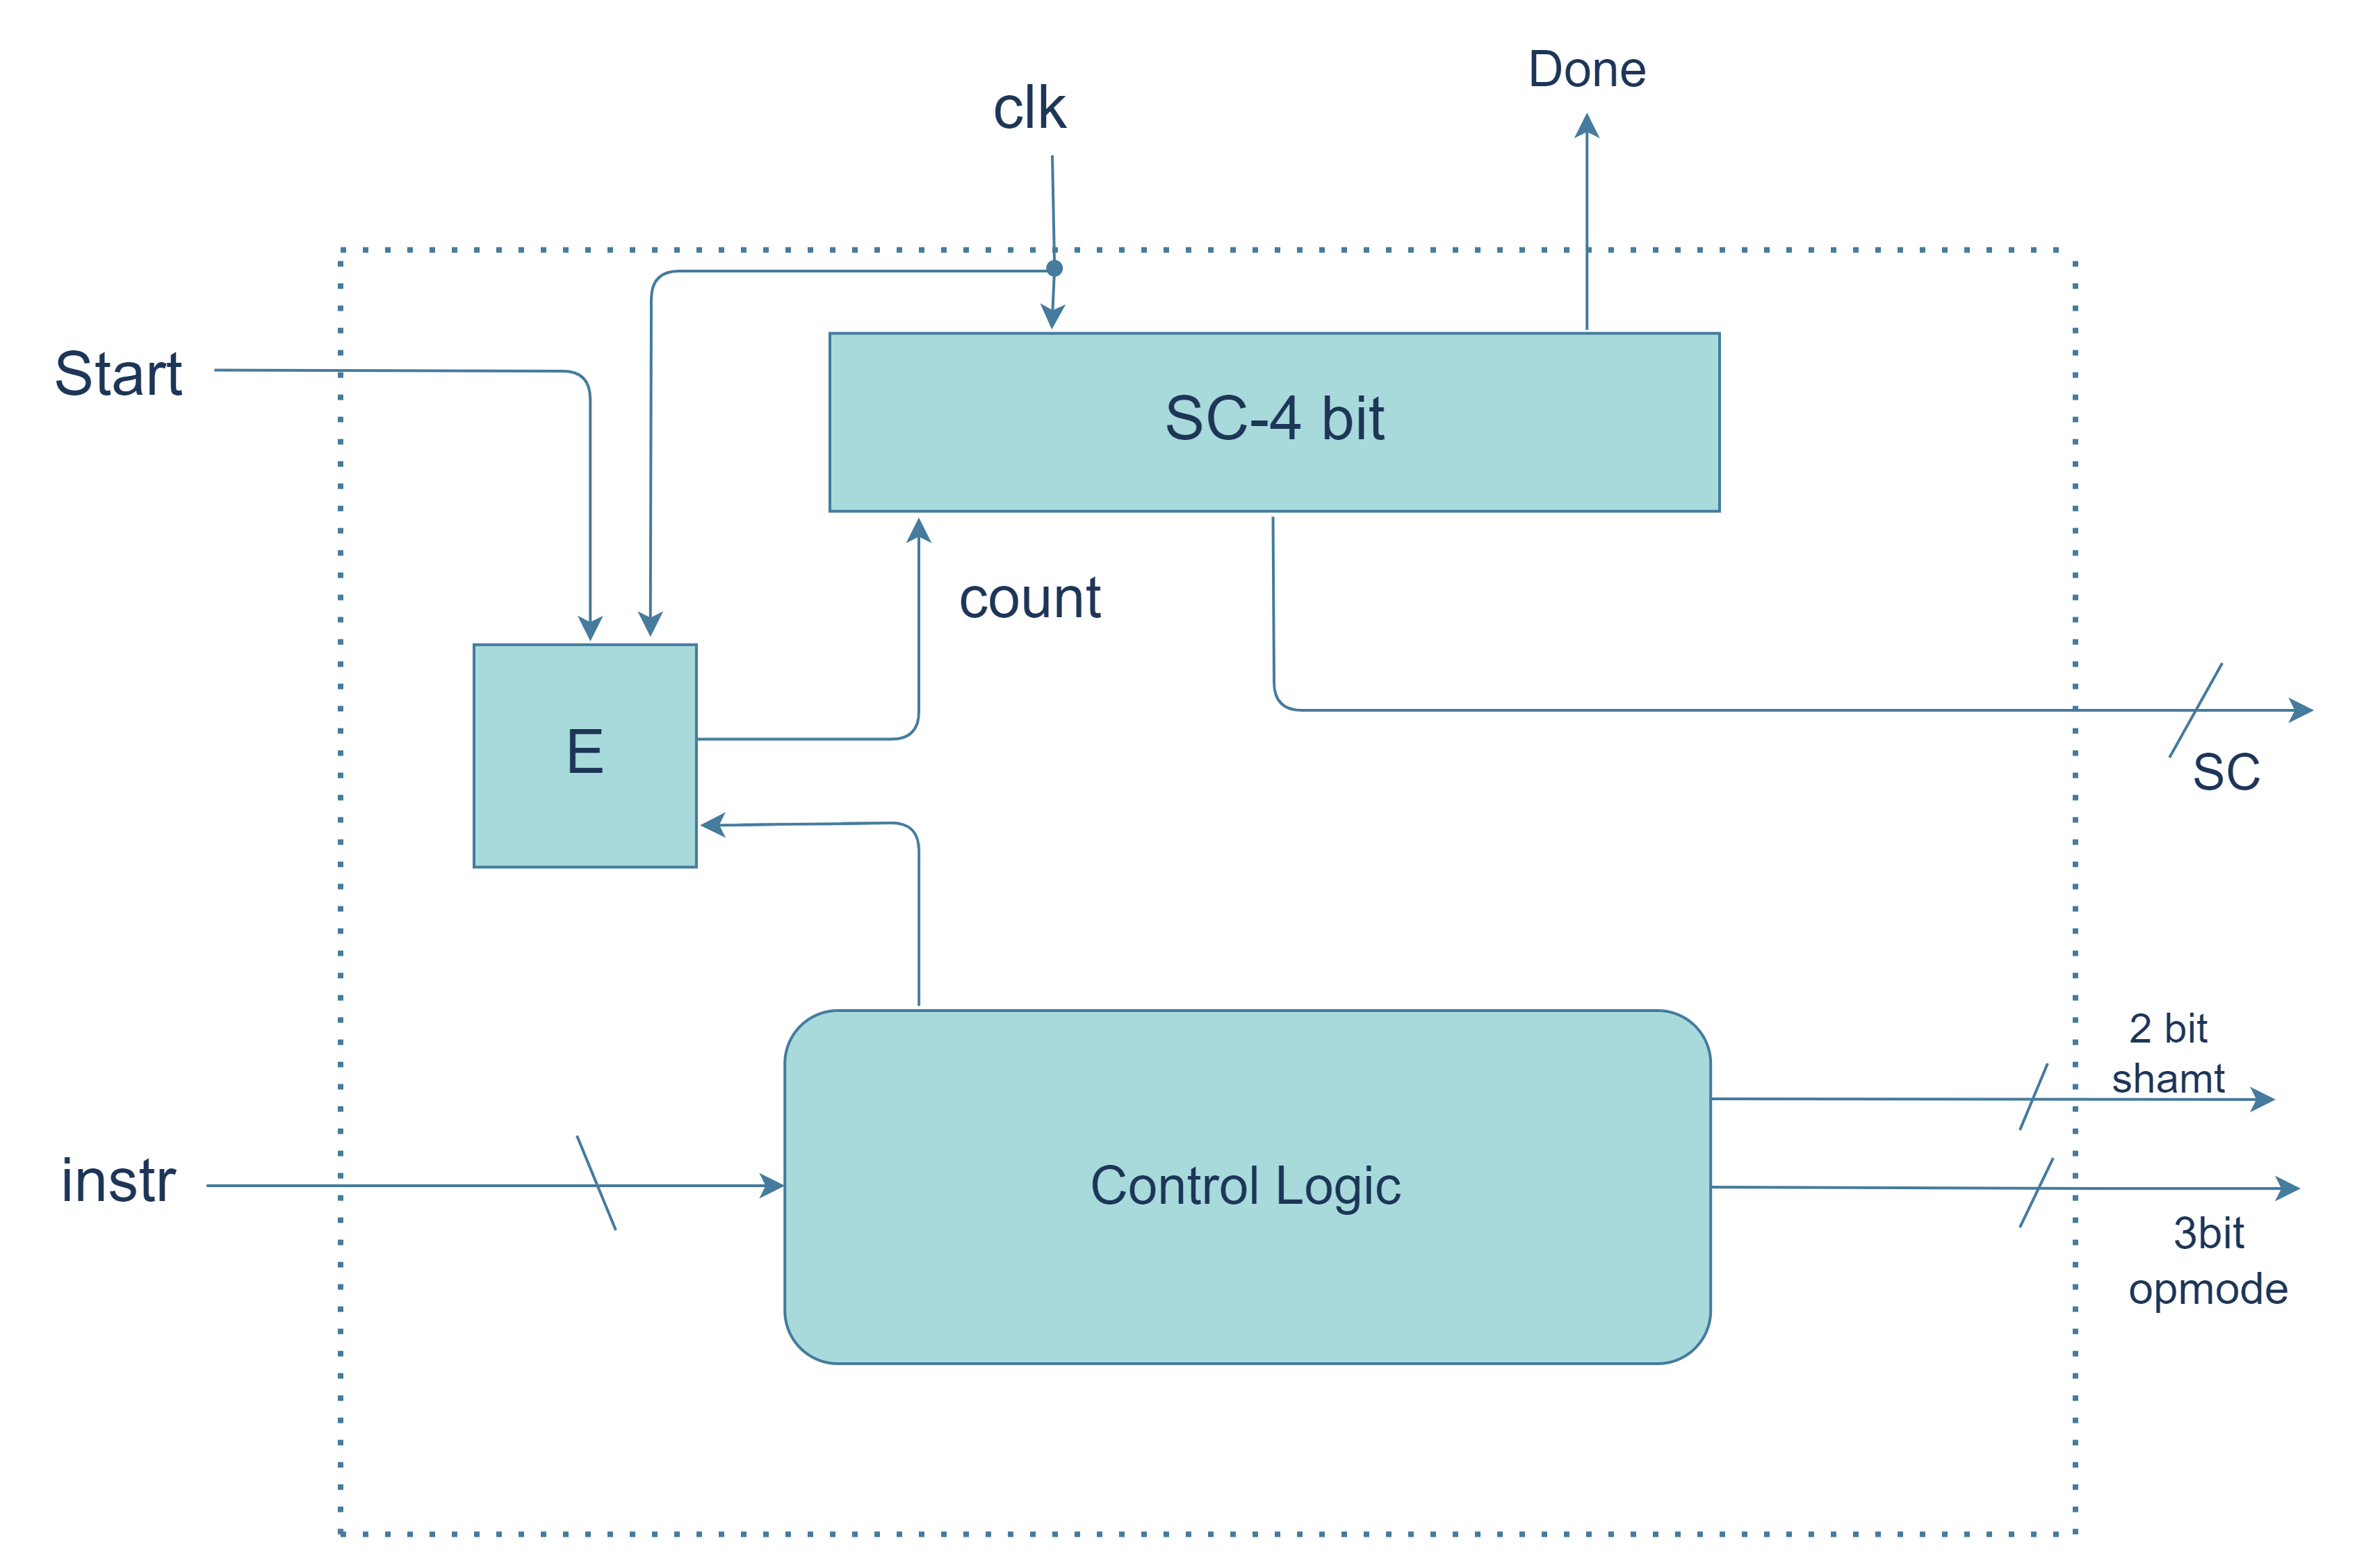
\includegraphics[scale=0.38]{controller.png}
\caption{Controller Schematic}
\label{controller}
\end{figure}

\begin{figure}[H]
\centering
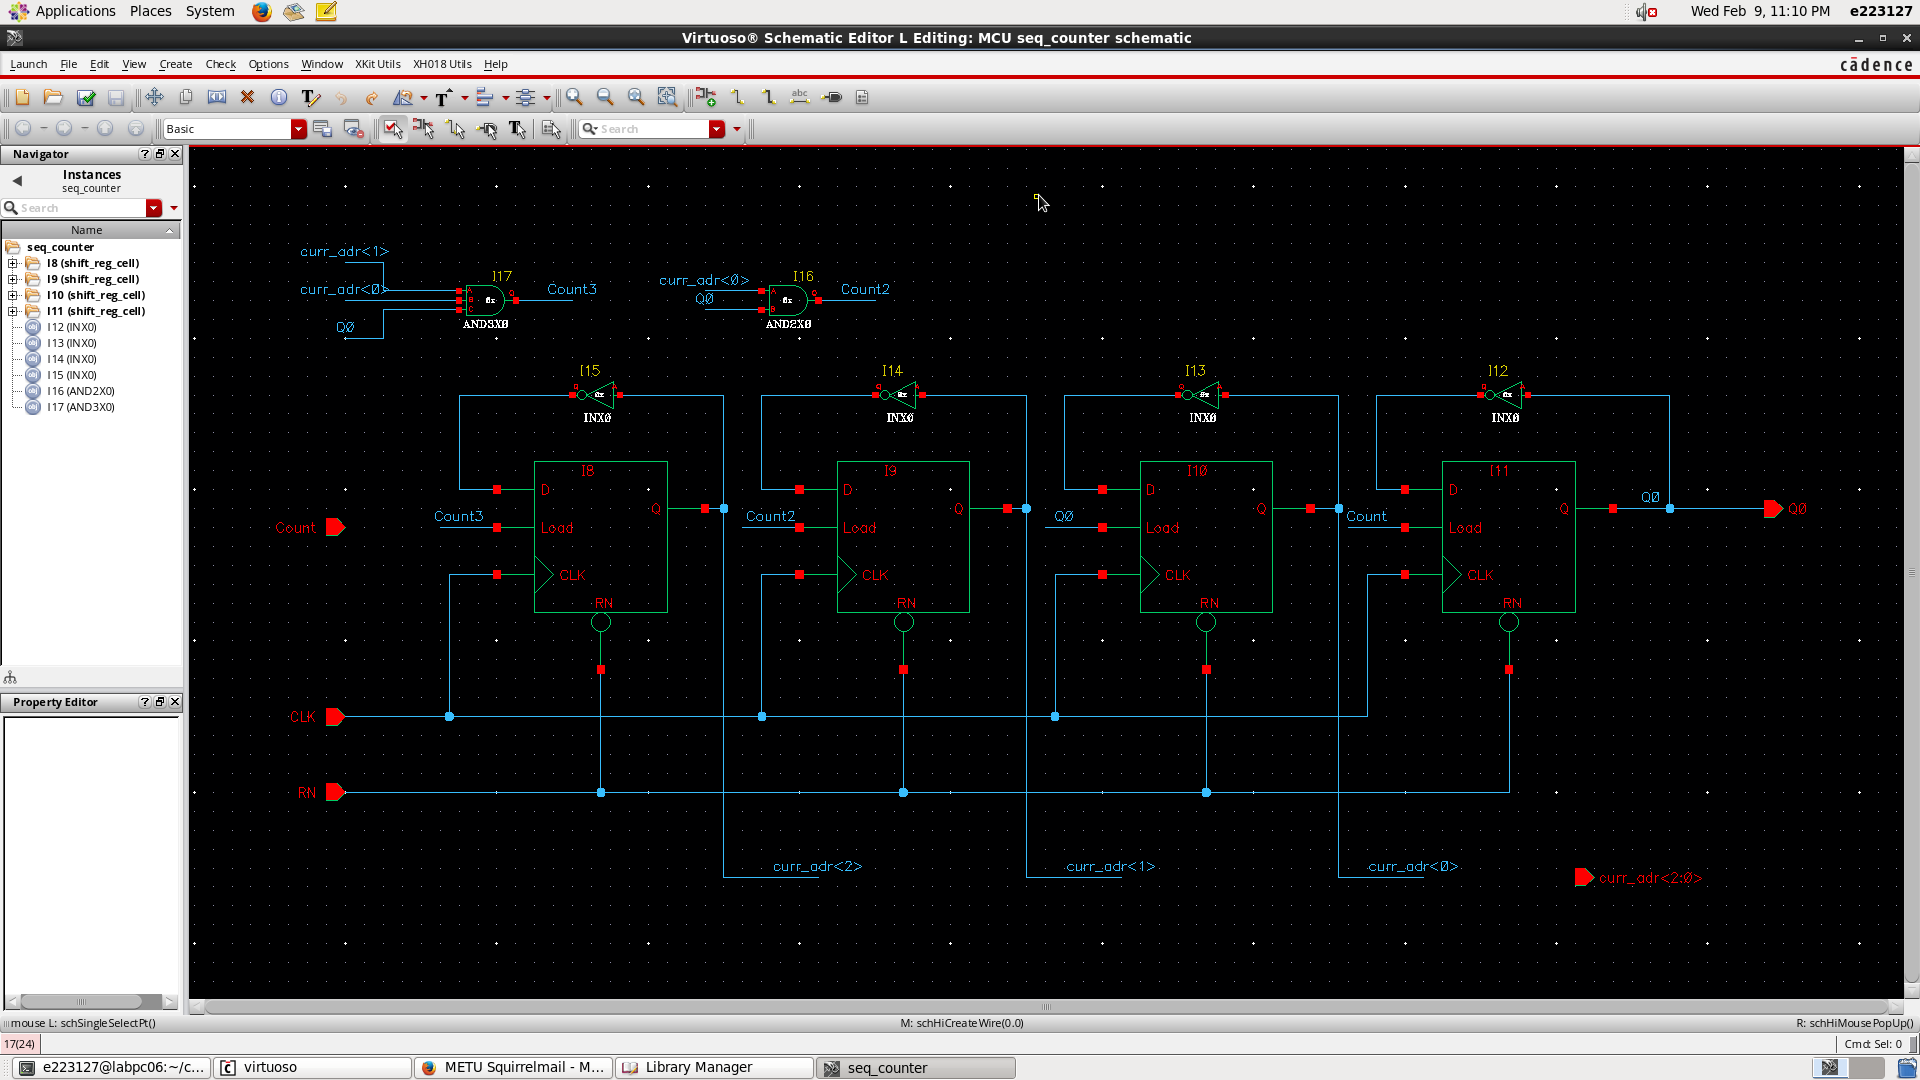
\includegraphics[scale=0.38]{seq_counter.png}
\caption{Sequence Counter Schematic}
\label{seq_cnt}
\end{figure}
\end{landscape}



\newpage
\subsection*{Output RAM}
The output unit of the ALU is the RAM. For this project, I designed a new RAM structure optimized for the specifications of the MCU. Figure \ref{ram} shows the schematic of the RAM.

\begin{itemize}
\item RAM, as the name suggests, is a random access memory type. That is, we should reach all the memory units whenever we want. Therefore, there should not be any CLK activity inside the RAM. Inputs and enable signals may be synchronized with the CLK. There is no CLK inputs to the RAM.

\item Current address input is supplied from the controller to read and write the necessary data to and from the correct places. Read and write decoders are used for this process.

\item There are 8 words in the RAM, each of which consists of 8 bits. These units are constructed using a D-latch. Write operation is enabled by the EN input of the D-latches provided by the XFAB.

\item We read the previous address of the RAM and write to the current address. This operation is conducted as follows:

\begin{itemize}
\item Read decoder enables the previous address of the current address input. For example, if the current address input is 100(4), we enable the 011(3) address from the RAM. Read operation is done by activating the output buffer of the D-latch. Read decoder schematic is shown in Figure \ref{read_dec_sch}.
\item This row, then, goes to the ALU where it is processed according to the current instruction.
\item Input to the RAM from the ALU is written to the enabled D-latch row. Write decoder is responsible for enabling the correct row of the D-latches for writing. Write decoder schematic can be seen in Figure \ref{write_dec_sch}.
\item Note that there is no independent path from every cell to and from the outputs and inputs. Same column cells are connected to the single line, which is activated by the decoders, just like any RAM structure. You can see this structure together with the decoders in the zoomed RAM structure in Figure \ref{ram_zoom}.
\end{itemize}

\item Active Low Reset input is provided to be on the safe side when we start the operation. Before every operation, a reset signal may be applied for safety.

\end{itemize}



\begin{landscape}
\pagestyle{empty}
\begin{figure}[H]
\centering
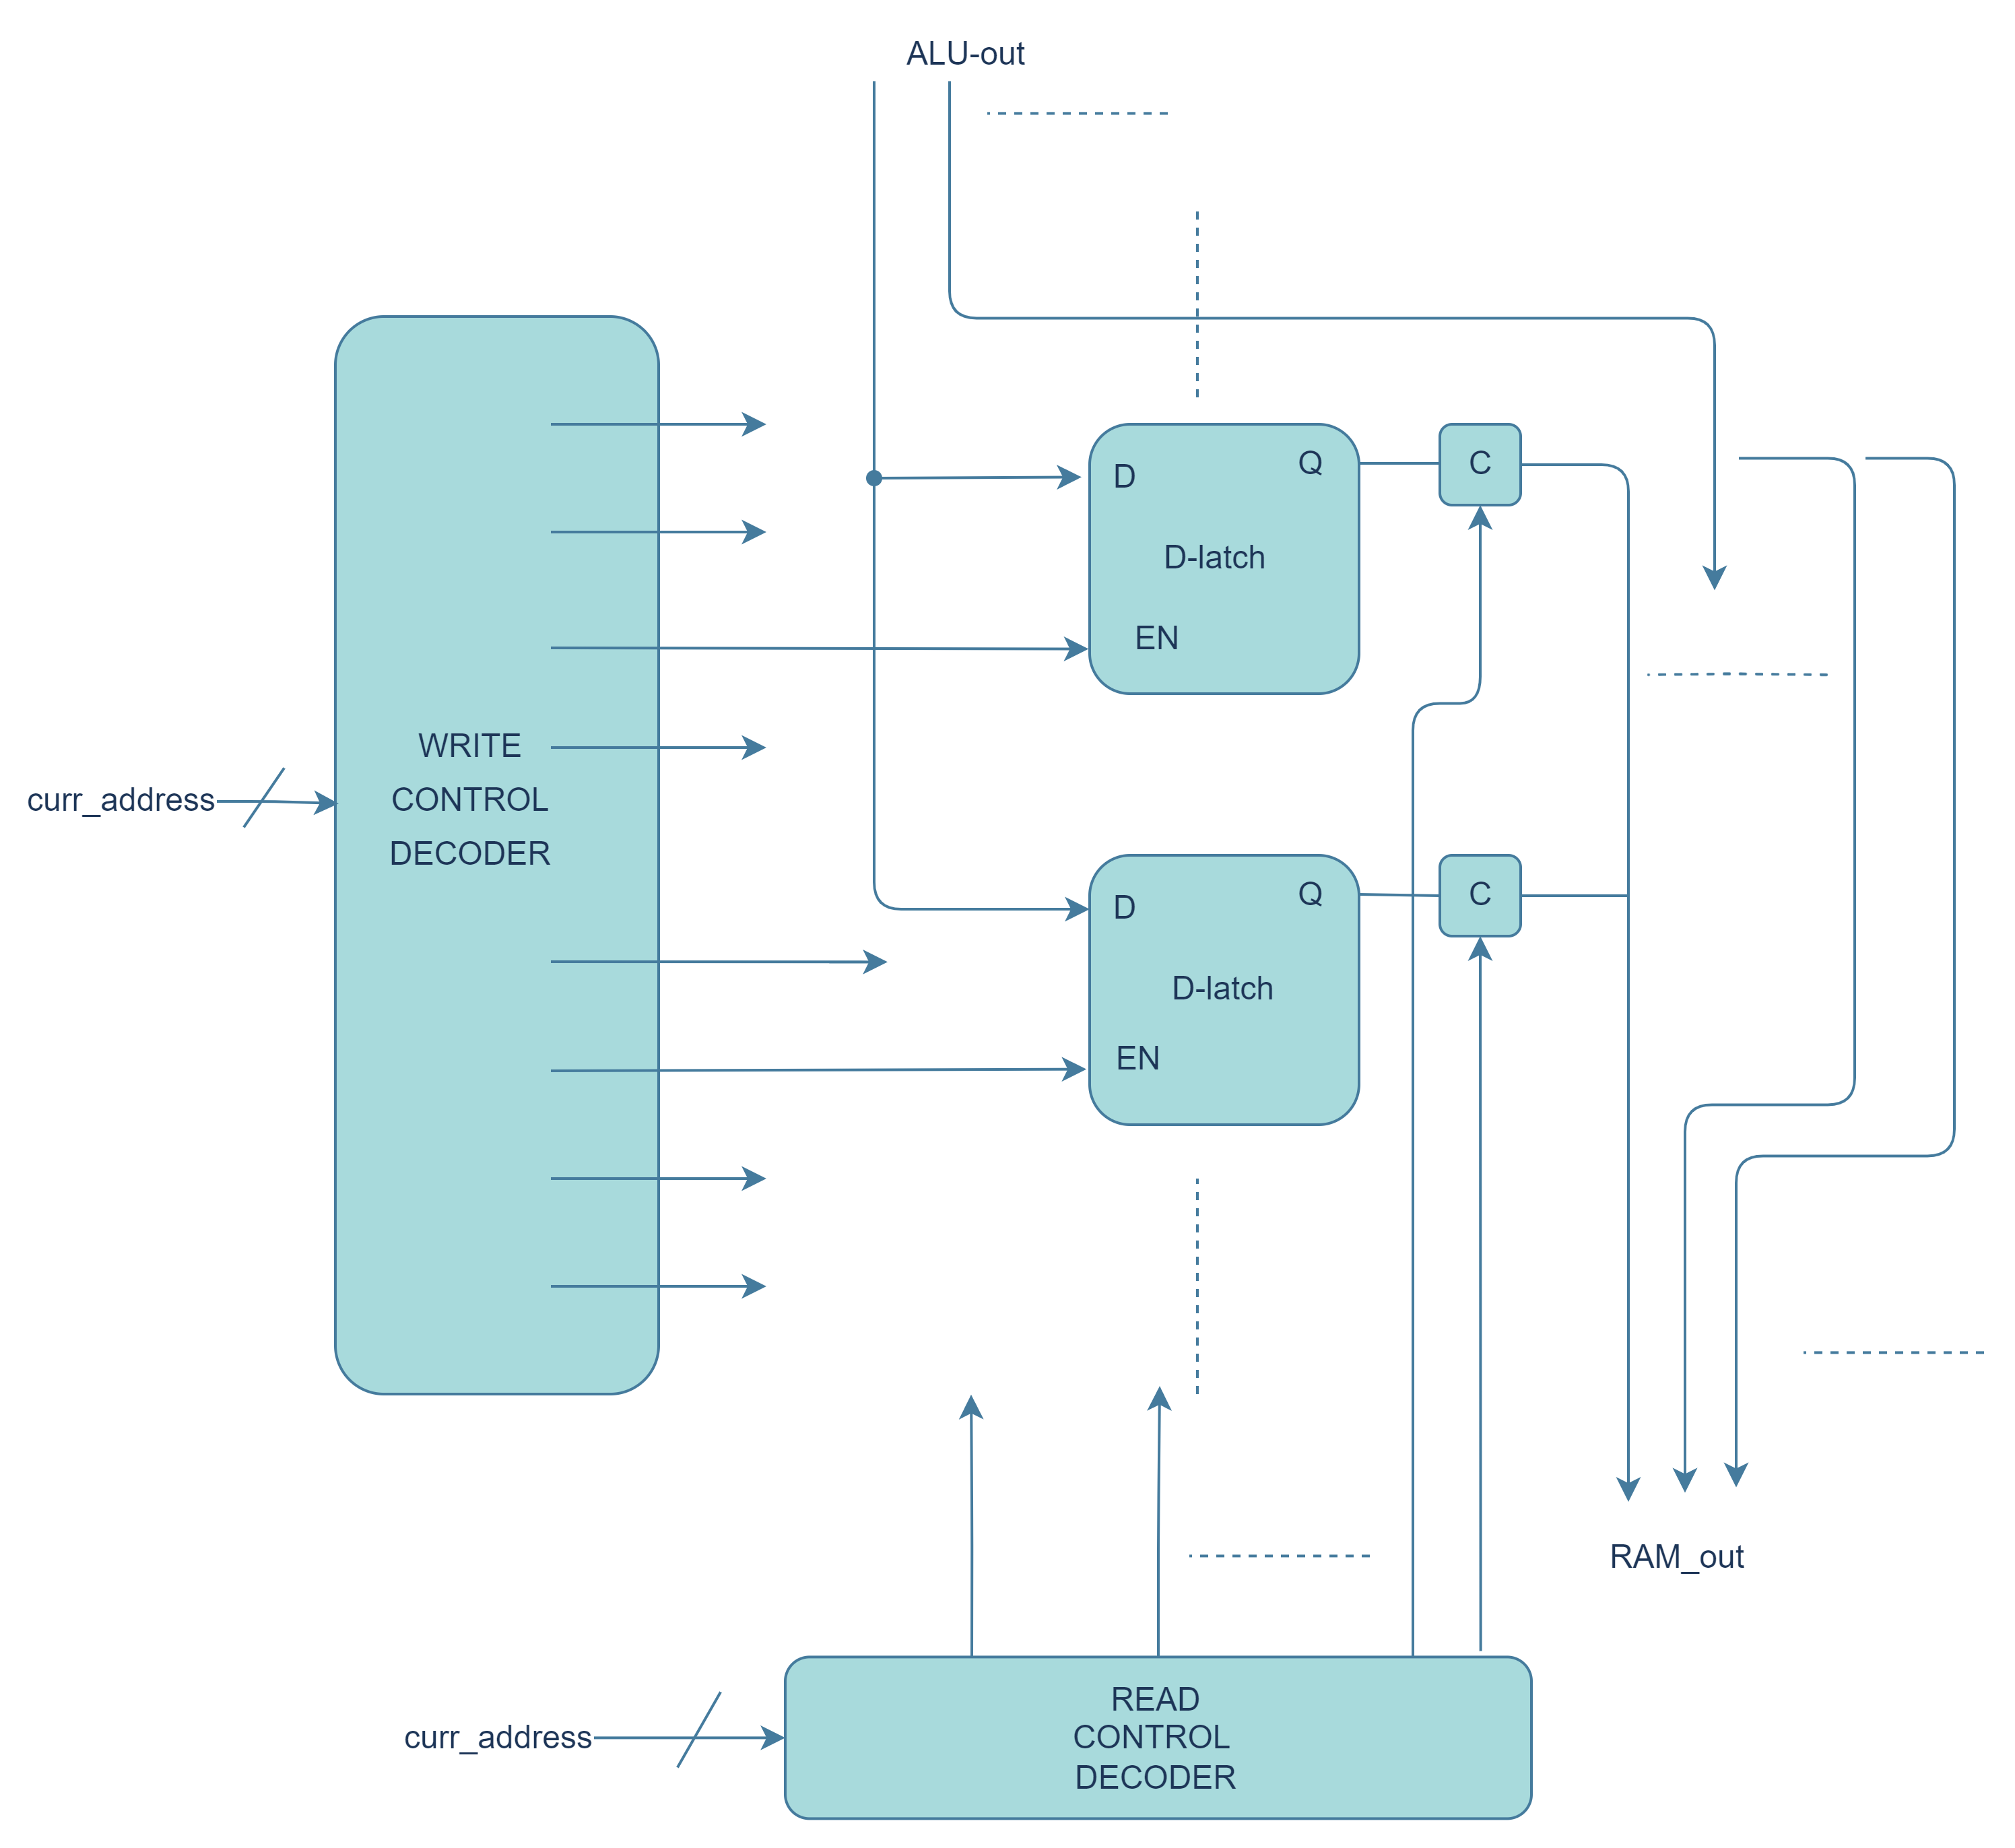
\includegraphics[scale=0.36]{ram.png}
\caption{Random Access Memory Schematic}
\label{ram}
\end{figure}

\begin{figure}[H]
\centering
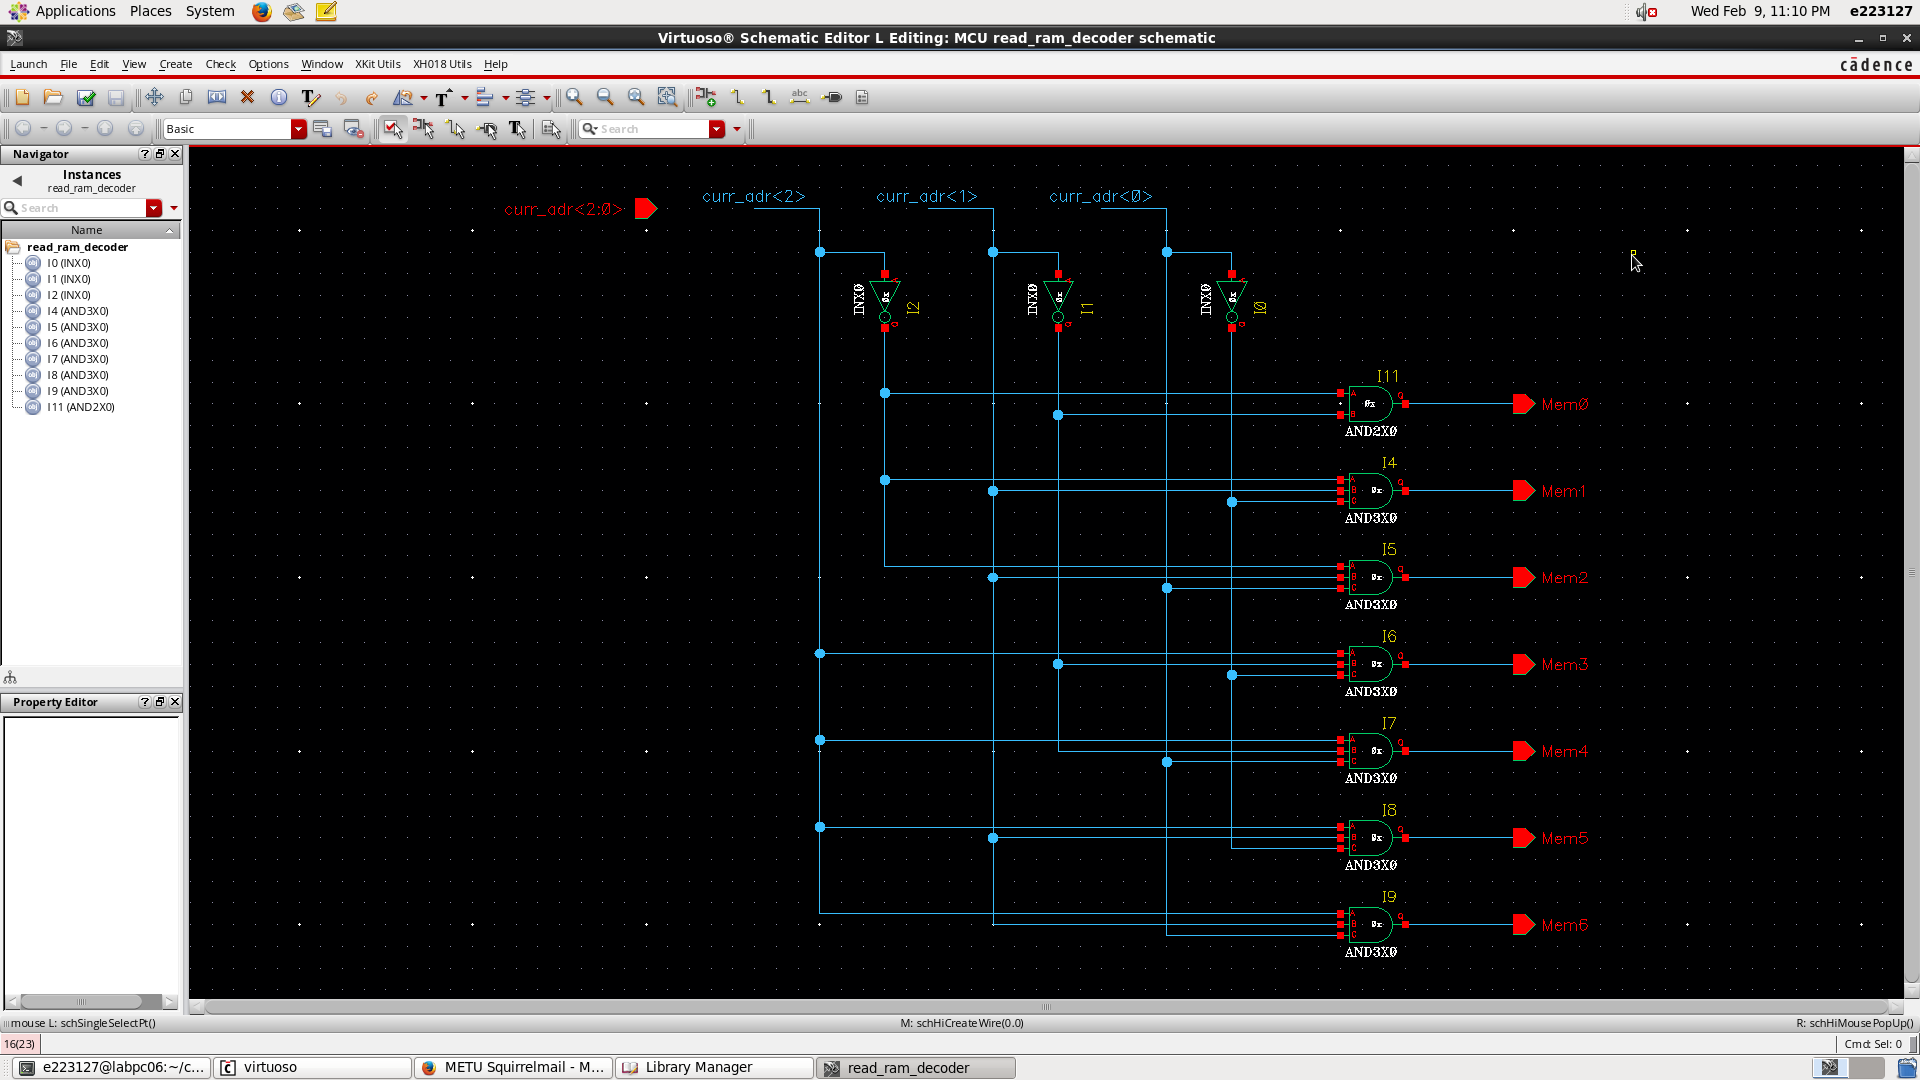
\includegraphics[scale=0.36]{read_decoder.png}
\caption{RAM Read Decoder Schematic}
\label{read_dec_sch}
\end{figure}


\begin{figure}[H]
\centering
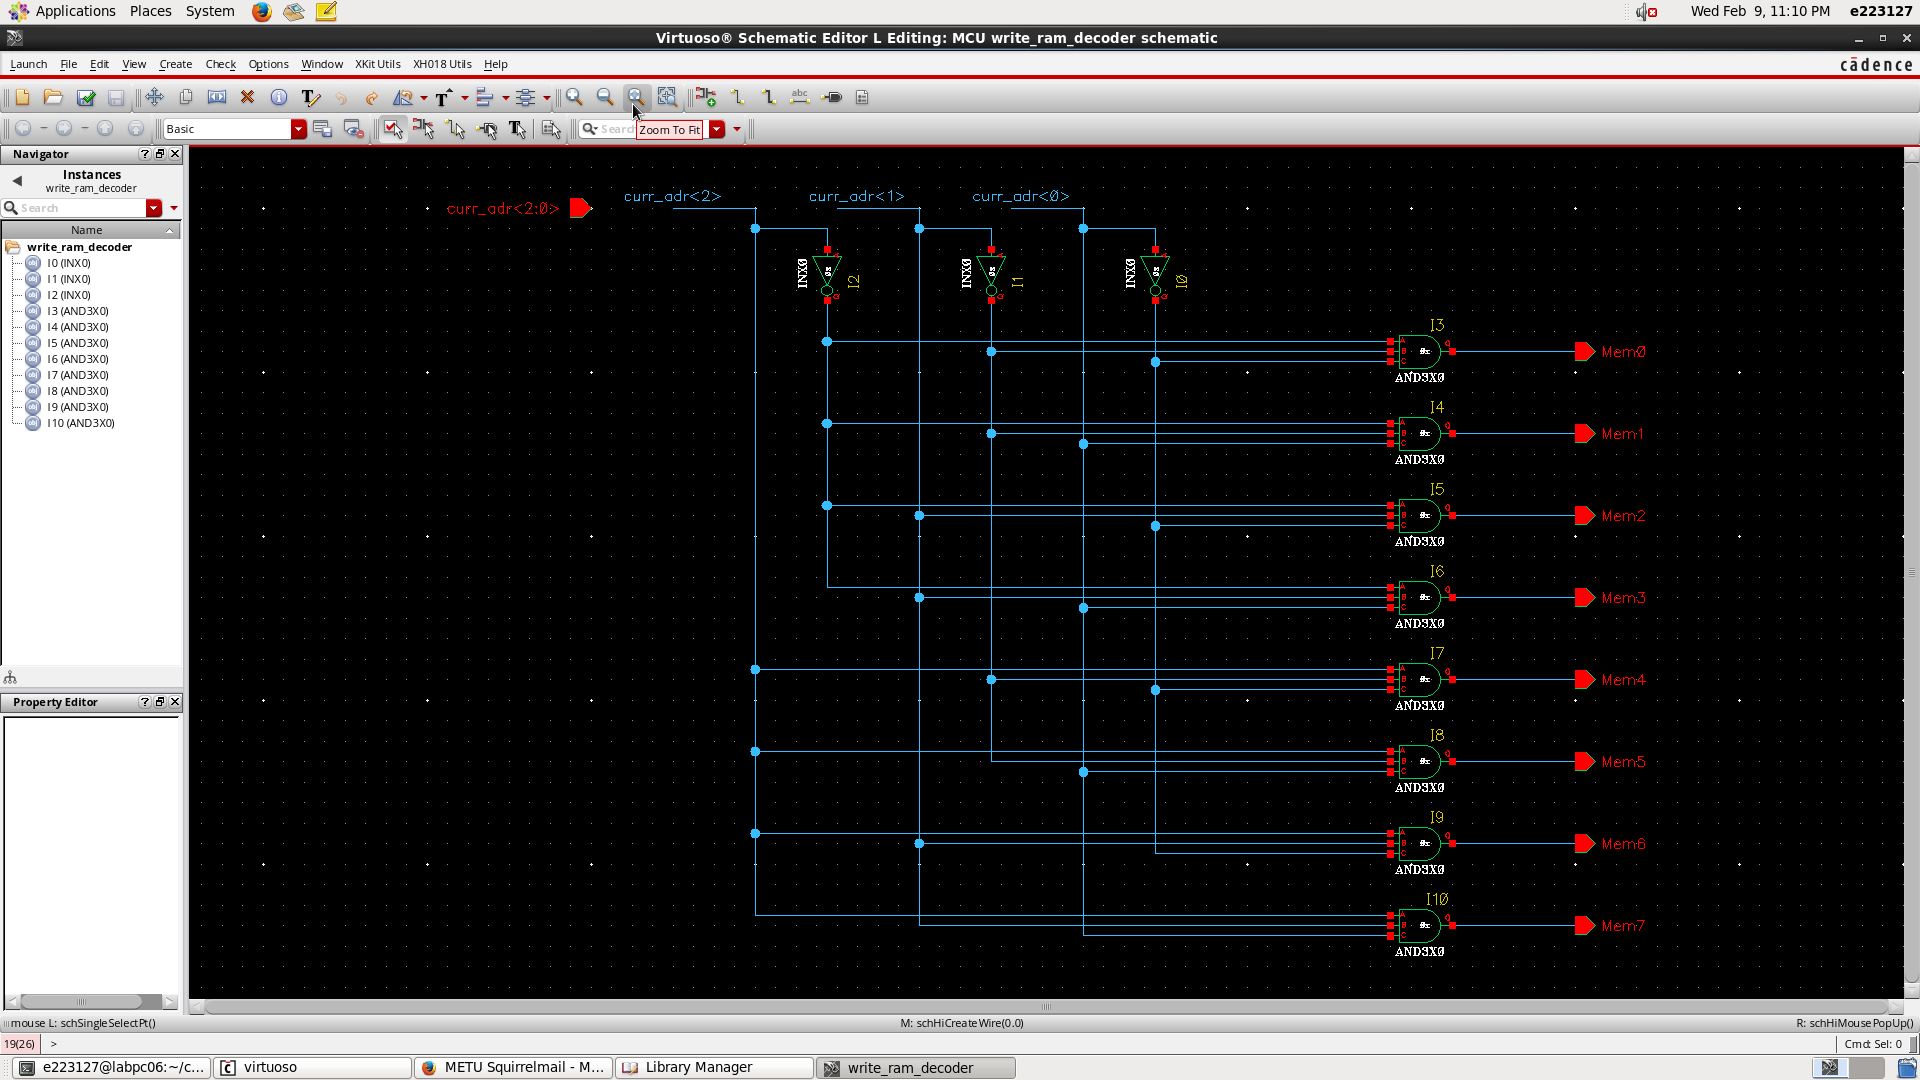
\includegraphics[scale=0.36]{write_decoder.png}
\caption{RAM Write Decoder Schematic}
\label{write_dec_sch}
\end{figure}

\begin{figure}[H]
\centering
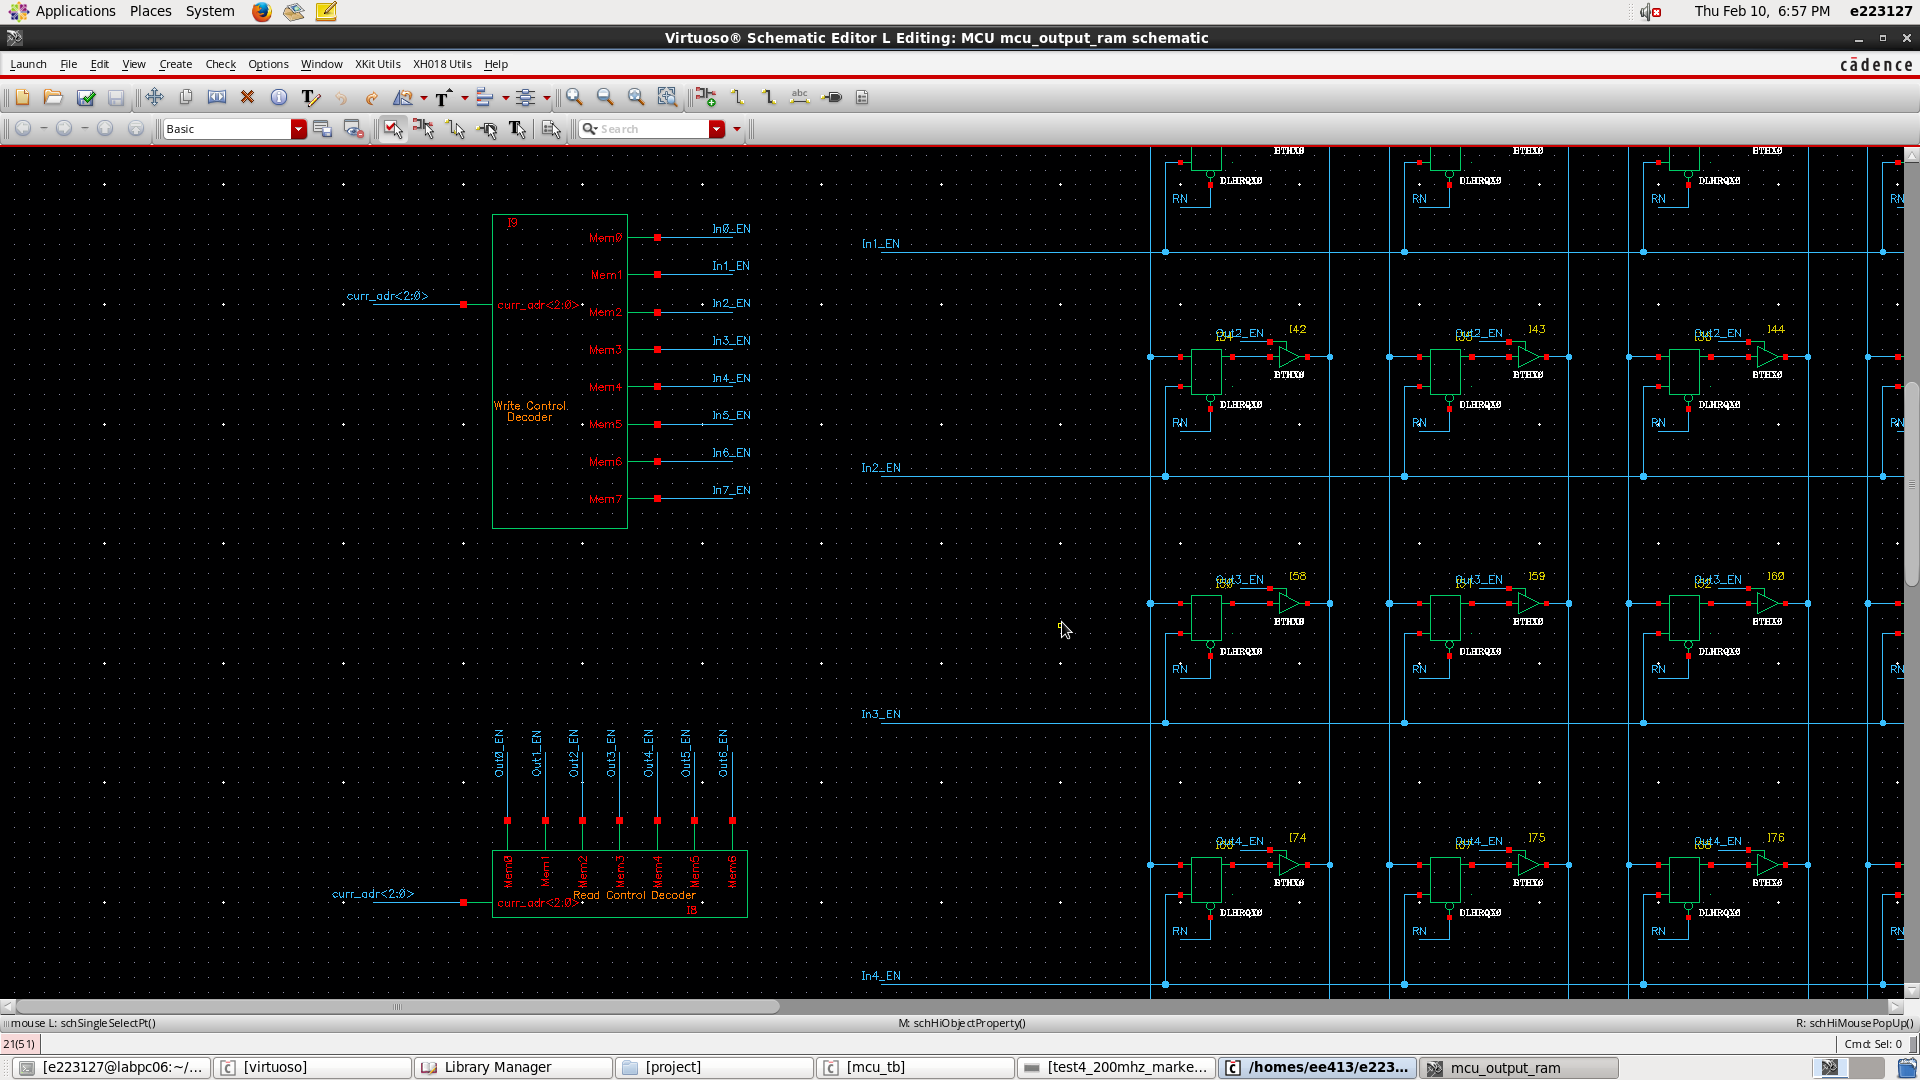
\includegraphics[scale=0.36]{ram_zoomed.png}
\caption{Random Access Memory Schematic - Zoomed}
\label{ram_zoom}
\end{figure}

\end{landscape}






%%%%%%%% sımulatıon results %%%%%%%%





\newpage
\subsection*{Simulation Results}

In IC world, testing is as important as design. A chip which is not properly tested is nothing but useless. Therefore, I have conducted an extensive test on the MCU. Below, you can find the different tests with their results and some performance criteria. Tests cover all of the 16 instructions. Frequency of operation and power dissipation figures are presented wherever possible. Testbench structure can be seen in Figure \ref{tb} in Appendix.

\subsubsection*{Test-1} %% test 6
This set subtracts two number using a long approach. \color{Green} SUCCESSFUL \color{Black}

\begin{itemize}
\item Frequency of Operation: 100 MHz
\item Power Dissipation: 302 $\mu$W (see the Figure \ref{test6_power} in Appendix)
\item Data\textsubscript{1} = 00010011 (19) 
\item Data\textsubscript{2} = 00010010 (18) 
\begin{table}[h]
\centering
\begin{tabular}{|c|c|c|c|}
\hline 
Order & Instruction & Operation & Expected Result \\ 
\hline 
1 & 0100 (4) & Load Reg2 & 19 \\ 
\hline 
2 & 0000 (0) & Idle & 19 \\ 
\hline 
3 & 1010 (10) & Subtract Reg2 & 1 \\ 
\hline 
4 & 1011 (11) & Subtract from Reg2 & 17 \\ 
\hline 
5 & 0110 (6) & Subtract from Reg1 & 2 \\ 
\hline 
6 & 0011 (3)& Shift Right & 1 \\ 
\hline 
7 & 1111 (15) & End & 1 \\ 
\hline 
\end{tabular} 
\caption{Instruction Set - Test 1}
\end{table}
\end{itemize}


\begin{figure}[H]
\centering
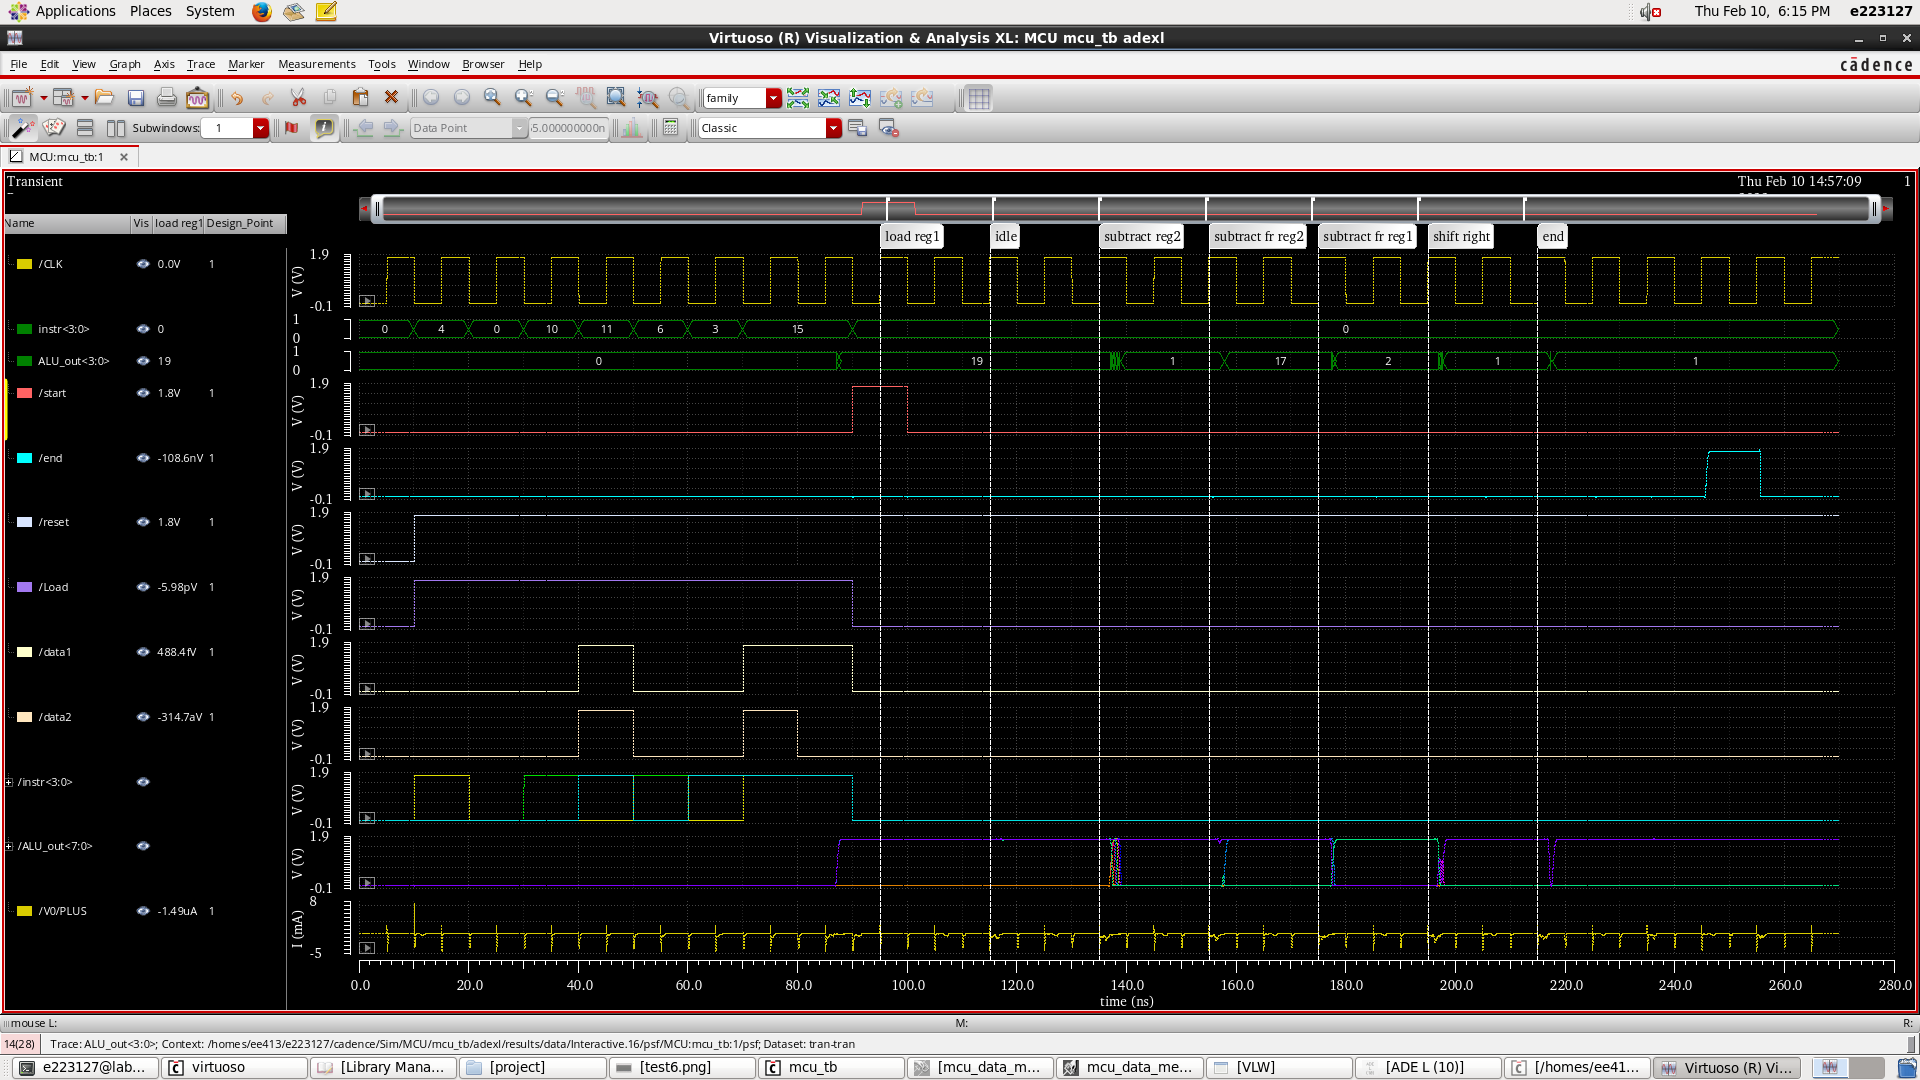
\includegraphics[scale=0.25]{tes6_marked_100mhz.png}
\caption{Simulation Result for Test 1}
\label{test6}
\end{figure}



\subsubsection*{Test-2} %% test-1
This test uses the load, subtraction and shift operations. \color{Green} SUCCESSFUL \color{Black}

\begin{itemize}
\item Frequency of Operation: 100 MHz
\item Power Dissipation: 313 $\mu$W (see the Figure \ref{test1_power} in Appendix)
\item Data\textsubscript{1} = 01111111 (127) 
\item Data\textsubscript{2} = 00100011 (35) 
\begin{table}[h]
\centering
\begin{tabular}{|c|c|c|c|}
\hline 
Order & Instruction & Operation & Expected Result \\ 
\hline 
1 & 0100 (4) & Load Reg1 & 127 \\ 
\hline 
2 & 1010 (10) & Subtract Reg2 & 92 \\ 
\hline 
3 & 1010 (10) & Subtract Reg2 & 57 \\ 
\hline 
4 & 1010 (10) & Subtract Reg2 & 22 \\ 
\hline 
5 & 0010 (2) & Shift Left & 44 \\ 
\hline 
6 & 0010 (2) & Shift Left & 88 \\ 
\hline 
7 & 0010 (2) & Shift Left & 176 \\ 
\hline 
8 & 1111 (15) & End & 176 \\ 
\hline 
\end{tabular} 
\caption{Instruction Set - Test 2}
\end{table}
\end{itemize}


\begin{figure}[H]
\centering
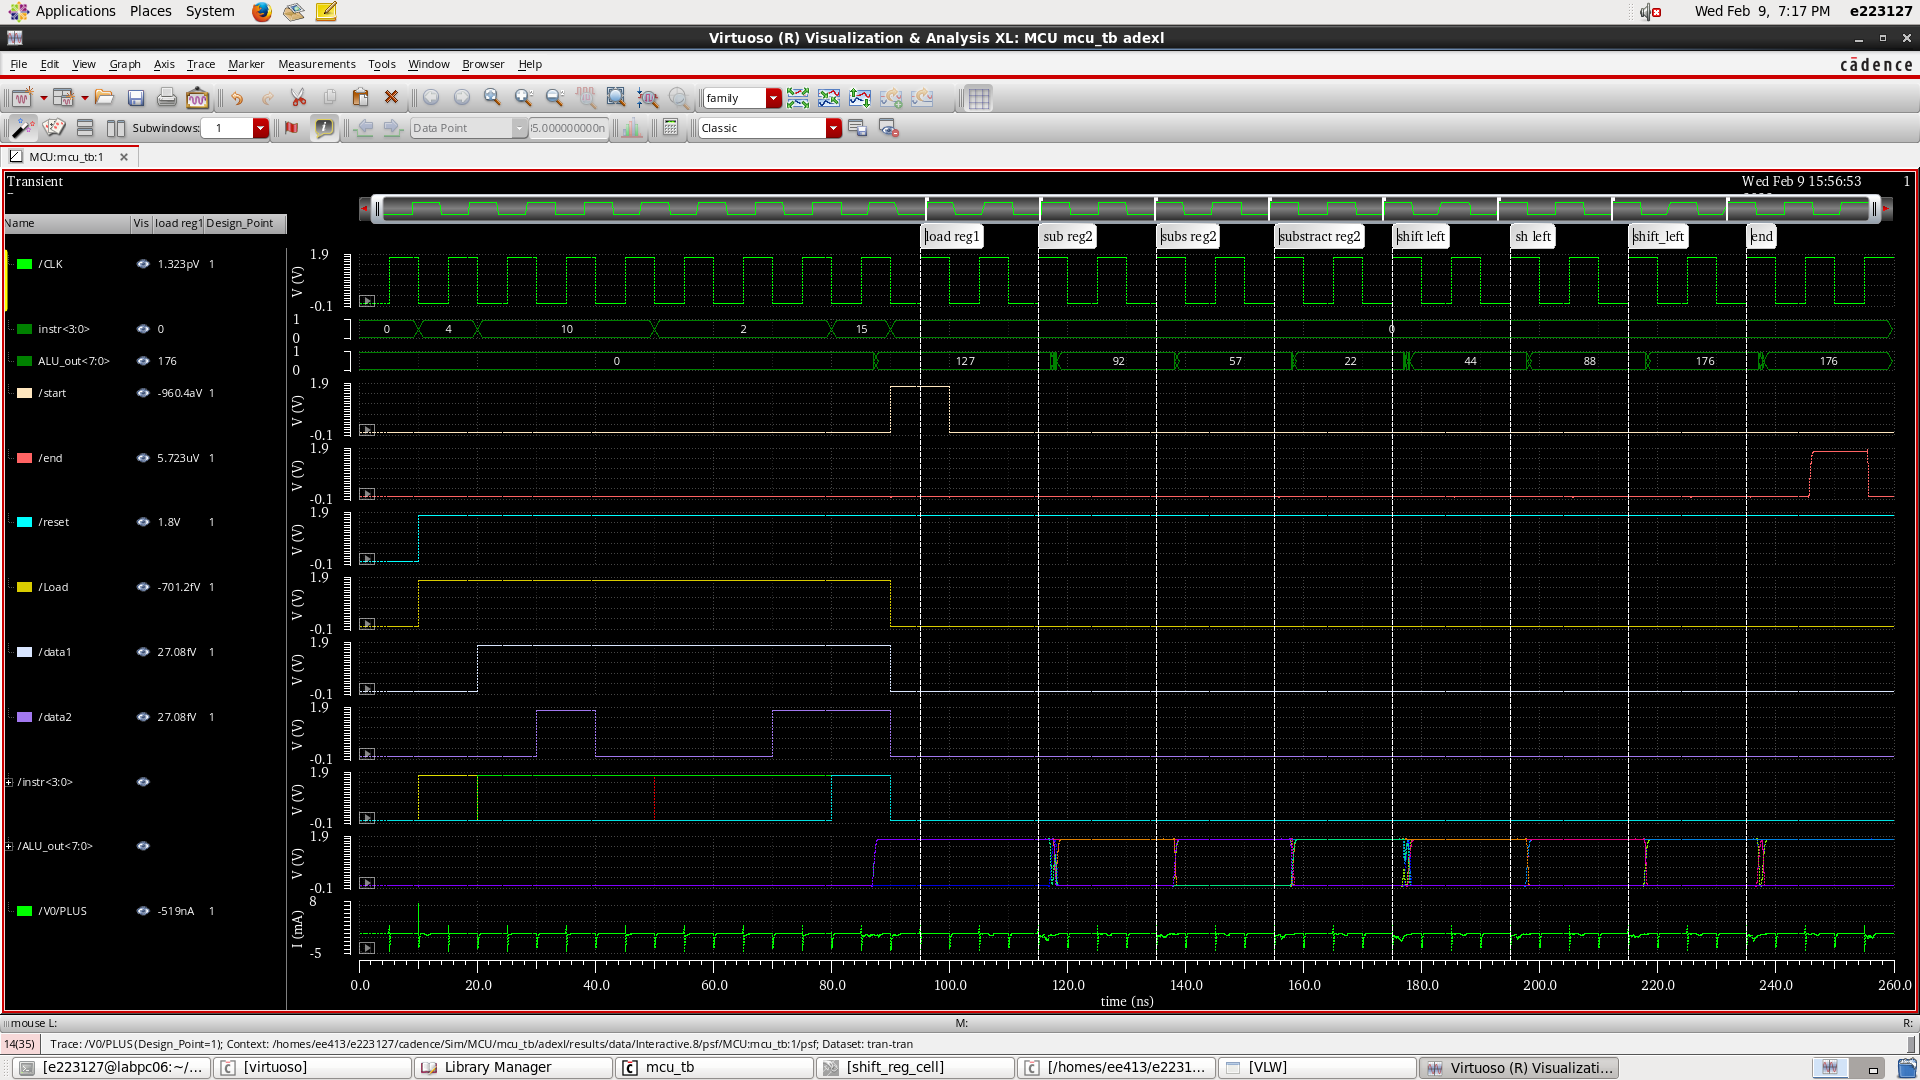
\includegraphics[scale=0.26]{test1_100mhz_marked.png}
\caption{Simulation Result for Test 2}
\label{test2}
\end{figure}





\subsubsection*{Test-3} %% test-2
This test uses the load, comparison and shift operations. \color{Green} SUCCESSFUL \color{Black}

\begin{itemize}
\item Frequency of Operation: 100 MHz
\item Power Dissipation: 339 $\mu$W (see the Figure \ref{test2_power} in Appendix)
\item Data\textsubscript{1} = 00101100 (44) 
\item Data\textsubscript{2} = 00010111 (23) 
\begin{table}[h]
\centering
\begin{tabular}{|c|c|c|c|}
\hline 
Order & Instruction & Operation & Expected Result \\ 
\hline 
1 & 0100 (4) & Load Reg1 & 44 \\ 
\hline 
2 & 0010 (2) & Shift Left & 88 \\ 
\hline 
3 & 0011 (3) & Shift Right & 44 \\ 
\hline 
4 & 1000 (8) & Compare w/ Reg1 & 44 \\ 
\hline 
5 & 1001 (9) & Load Reg2 & 23 \\ 
\hline 
6 & 0010 (2) & Shift Left & 46 \\ 
\hline 
7 & 0011 (3) & Shift Right & 23 \\ 
\hline 
8 & 1111 (15) & End & 23 \\ 
\hline 
\end{tabular} 
\caption{Instruction Set - Test 3}
\end{table}
\end{itemize}


\begin{figure}[H]
\centering
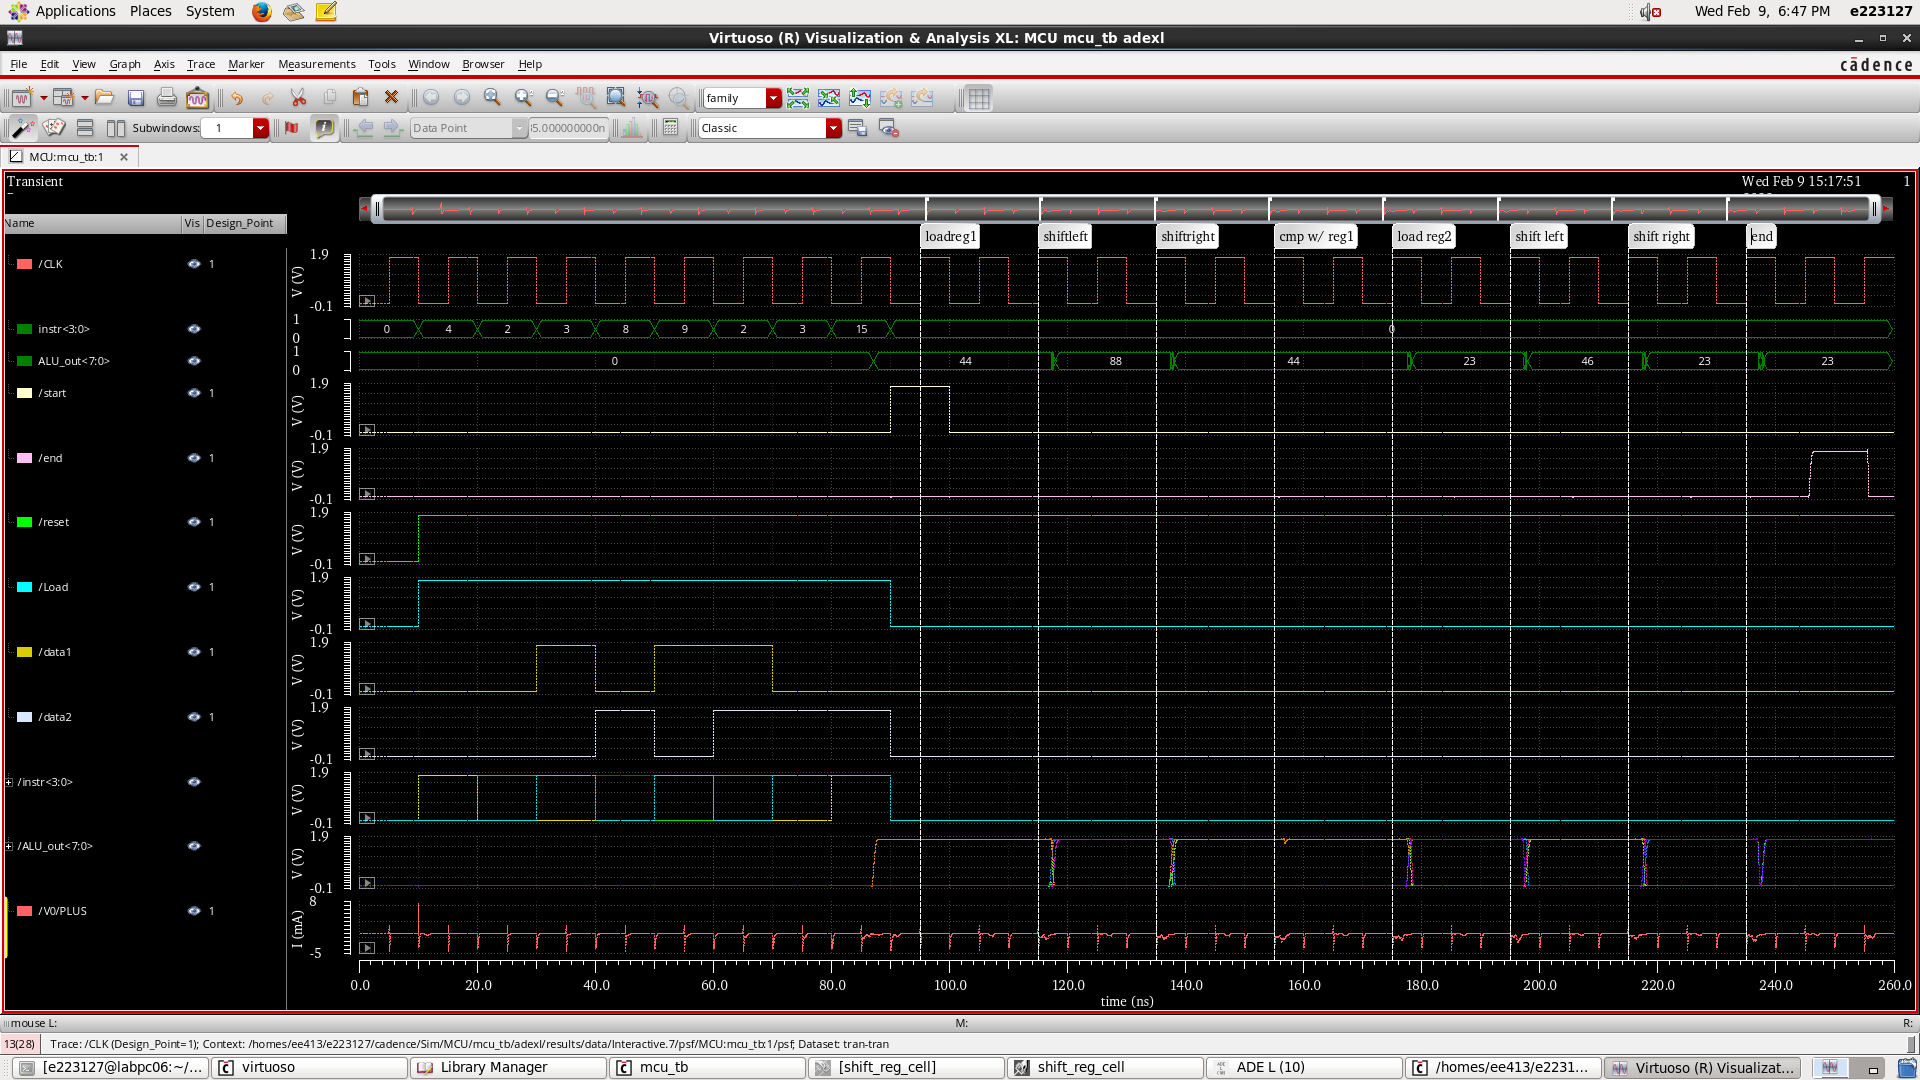
\includegraphics[scale=0.27]{test2_100mhz_marked.png}
\caption{Simulation Result for Test 3}
\label{test3}
\end{figure}




\subsubsection*{Test-4} %% test-4
This test compares the two numbers and gives the 4$\times$bigger one via the long way. Note that this test is conducted in 200MHz. Accordingly, power dissipation is almost doubled.  \color{Green} SUCCESSFUL \color{Black}

\begin{itemize}
\item Frequency of Operation: 200 MHz
\item Power Dissipation: 577 $\mu$W (see the Figure \ref{test4_power} in Appendix)
\item Data\textsubscript{1} = 00000110 (6) 
\item Data\textsubscript{2} = 00011110 (30) 
\begin{table}[h]
\centering
\begin{tabular}{|c|c|c|c|}
\hline 
Order & Instruction & Operation & Expected Result \\ 
\hline 
1 & 1001 (9) & Load Reg2 & 30 \\ 
\hline 
2 & 1101 (13) & Compare w/ Reg2 & 30 \\ 
\hline 
3 & 1000 (8) & Compare w/ Reg1 & 30 \\ 
\hline 
4 & 0010 (2) & Shift Left & 60 \\ 
\hline 
5 & 0010 (2) & Shift Left & 120 \\ 
\hline 
6 & 0011 (3) & Shift Right & 60 \\ 
\hline 
7 & 0010 (2) & Shift Left & 120 \\ 
\hline 
8 & 1111 (15) & End & 120 \\ 
\hline 
\end{tabular} 
\caption{Instruction Set - Test 4}
\end{table}
\end{itemize}


\begin{figure}[H]
\centering
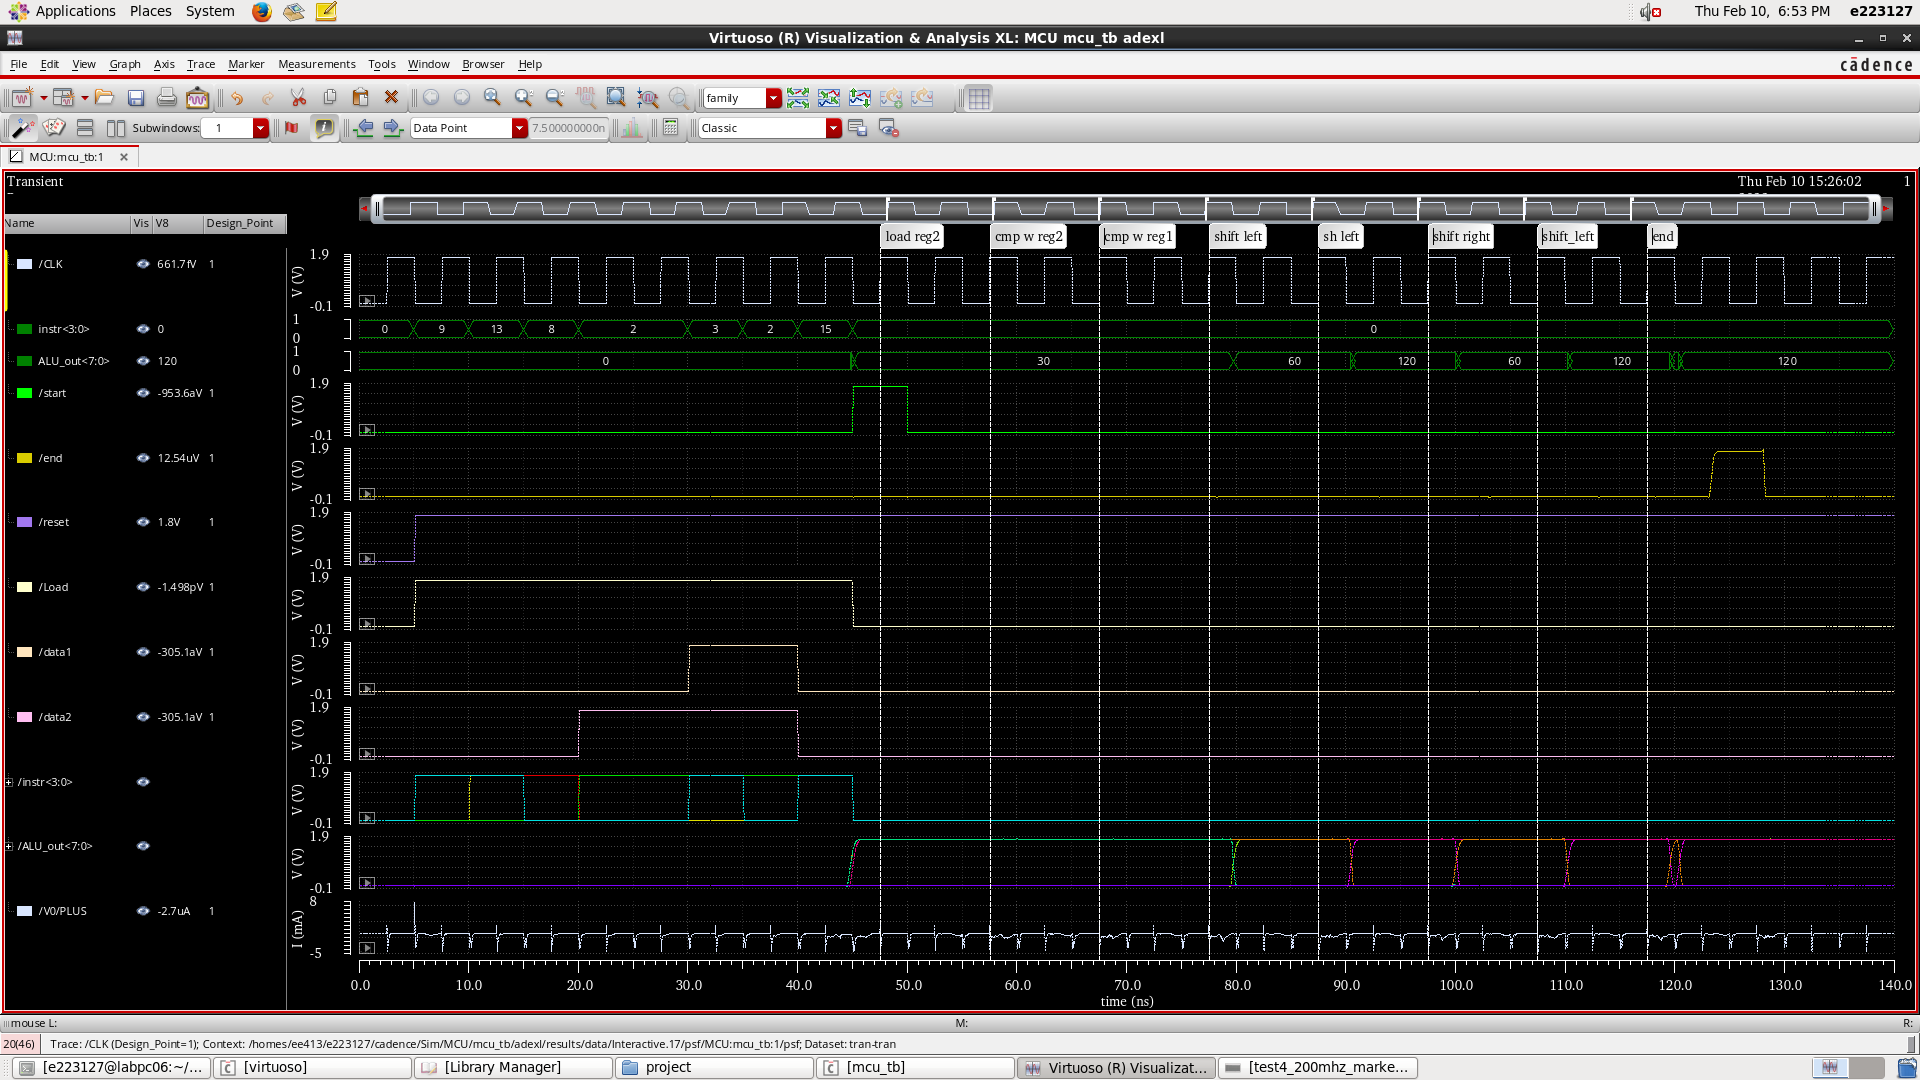
\includegraphics[scale=0.27]{test4_marked_200mhz.png}
\caption{Simulation Result for Test 4}
\label{test4}
\end{figure}





\subsubsection*{Test-5} %% test-3
This test uses load, add, subtract, set and reset instructions. Note that this test is conducted in 200MHz. Accordingly, power dissipation is almost doubled.  \color{Green} SUCCESSFUL \color{Black}

\begin{itemize}
\item Frequency of Operation: 200 MHz
\item Power Dissipation: 654 $\mu$W (see the Figure \ref{test3_power} in Appendix)
\item Data\textsubscript{1} = 01111110 (126) 
\item Data\textsubscript{2} = 10000001 (129) 
\begin{table}[h]
\centering
\begin{tabular}{|c|c|c|c|}
\hline 
Order & Instruction & Operation & Expected Result \\ 
\hline 
1 & 0100 (4) & Load Reg1 & 126 \\ 
\hline 
2 & 1100 (12) & Add Reg2 & 255 \\ 
\hline 
3 & 0101 (5) & Subtract Reg1 & 129 \\ 
\hline 
4 & 1011 (11) & Subtract from Reg2 & 0 \\ 
\hline 
5 & 0001 (1) & Set & 255 \\ 
\hline 
6 & 1110 (14) & Reset & 0 \\ 
\hline 
7 & 1111 (15) & End & 0 \\ 
\hline 
8 & 1111 (15) & End & 0 \\ 
\hline 
\end{tabular} 
\caption{Instruction Set - Test 5}
\end{table}
\end{itemize}


\begin{figure}[H]
\centering
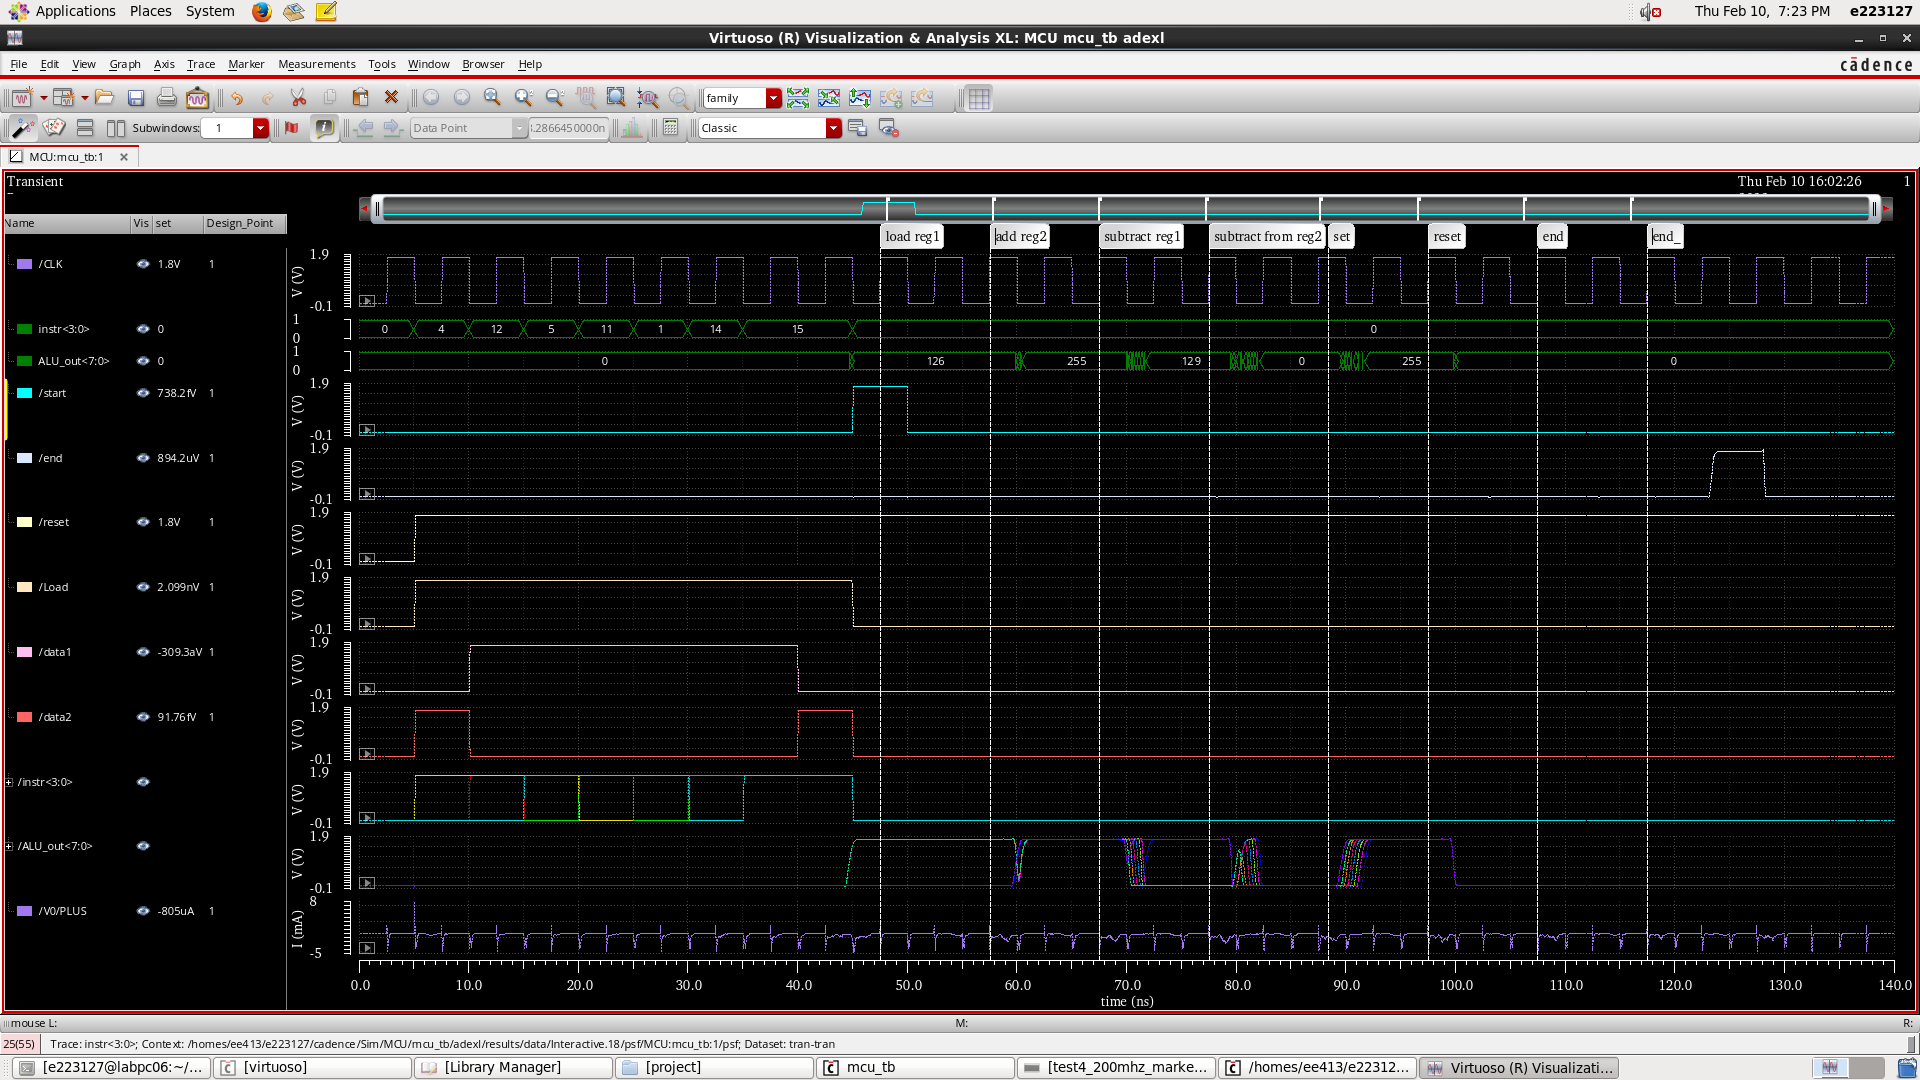
\includegraphics[scale=0.27]{test3_200mhz_marked.png}
\caption{Simulation Result for Test 5}
\label{test5}
\end{figure}



\subsubsection*{Test-6} %% test-5
This test uses compare, shift, add, subtract, set and reset instructions.\color{Green} SUCCESSFUL \color{Black}

\begin{itemize}
\item Frequency of Operation: 100 MHz
\item Data\textsubscript{1} = 01111111 (127) 
\item Data\textsubscript{2} = 11111111 (255) 
\begin{table}[h]
\centering
\begin{tabular}{|c|c|c|c|}
\hline 
Order & Instruction & Operation & Expected Result \\ 
\hline 
1 & 0001 (1) & Set & 255 \\ 
\hline 
2 & 1101 (13) & Compare w/ Reg2 & 255 \\ 
\hline 
3 & 0101 (5) & Subtract Reg1 & 128 \\ 
\hline 
4 & 1000 (8) & Compare w/ Reg1 & 128 \\ 
\hline 
5 & 0011 (3) & Shift Right & 64 \\ 
\hline 
6 & 1000 (8) & Compare w/ Reg1 & 127 \\ 
\hline 
7 & 1100 (12) & Add Reg2 & 126 (equal to 127-1) \\ 
\hline 
8 & 1111 (15) & End & 126 \\ 
\hline 
\end{tabular} 
\caption{Instruction Set - Test 6}
\end{table}
\end{itemize}


\begin{figure}[H]
\centering
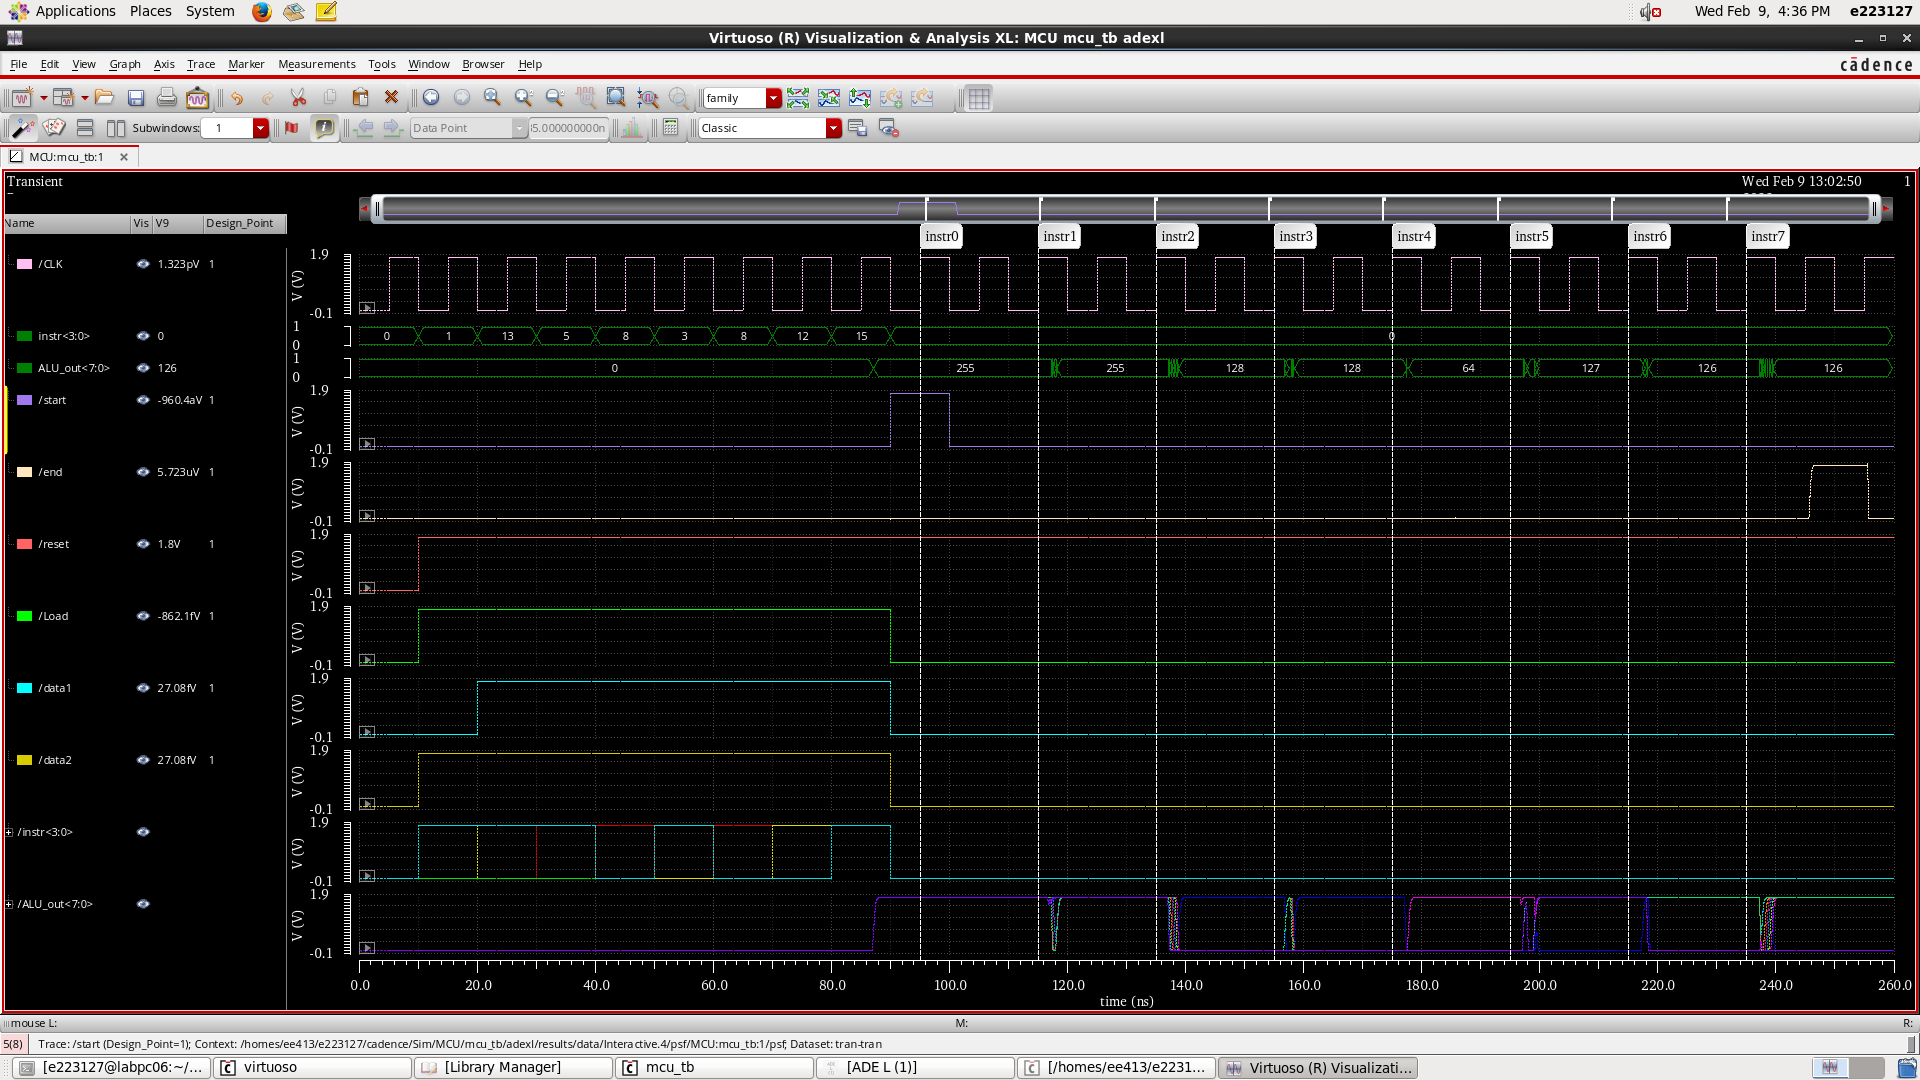
\includegraphics[scale=0.27]{test5_marked.png}
\caption{Simulation Result for Test 6}
\label{test6}
\end{figure}



%%%%%%%  LAYOUTS %%%%%%%%%%%






\newpage
\subsection*{Layouts}
\label{lay}
After the schematics and verification of the design via extensive test, layout of the MCU is started. Due to the limited time, I could not complete the entire MCU layout. However, some blocks are completed and presented in the following pages.

\subsubsection*{Instruction Memory}
Instruction memory layout is presented in Figure \ref{instruction_lay}. It consists of 32 register cell(D-FF with MUX) and an OR gate for two different Load signals. \\

DRC and LVS results are shown in Figure \ref{instruction_drc} and Figure \ref{instruction_lvs}, respectively. Analog extracted view can be seen in Figure \ref{instruction_extracted}.


\subsubsection*{Data Memory}

Data Memory consists of 16 register cell and 8 2$\times$1 MUX. Data memory layout is presented in Figure \ref{data_lay}. \\

DRC and LVS results are shown in Figure \ref{data_drc} and Figure \ref{data_lvs}, respectively. Analog extracted view can be seen in Figure \ref{data_extracted}.

\begin{landscape}
\pagestyle{empty}

\begin{figure}[H]
\centering
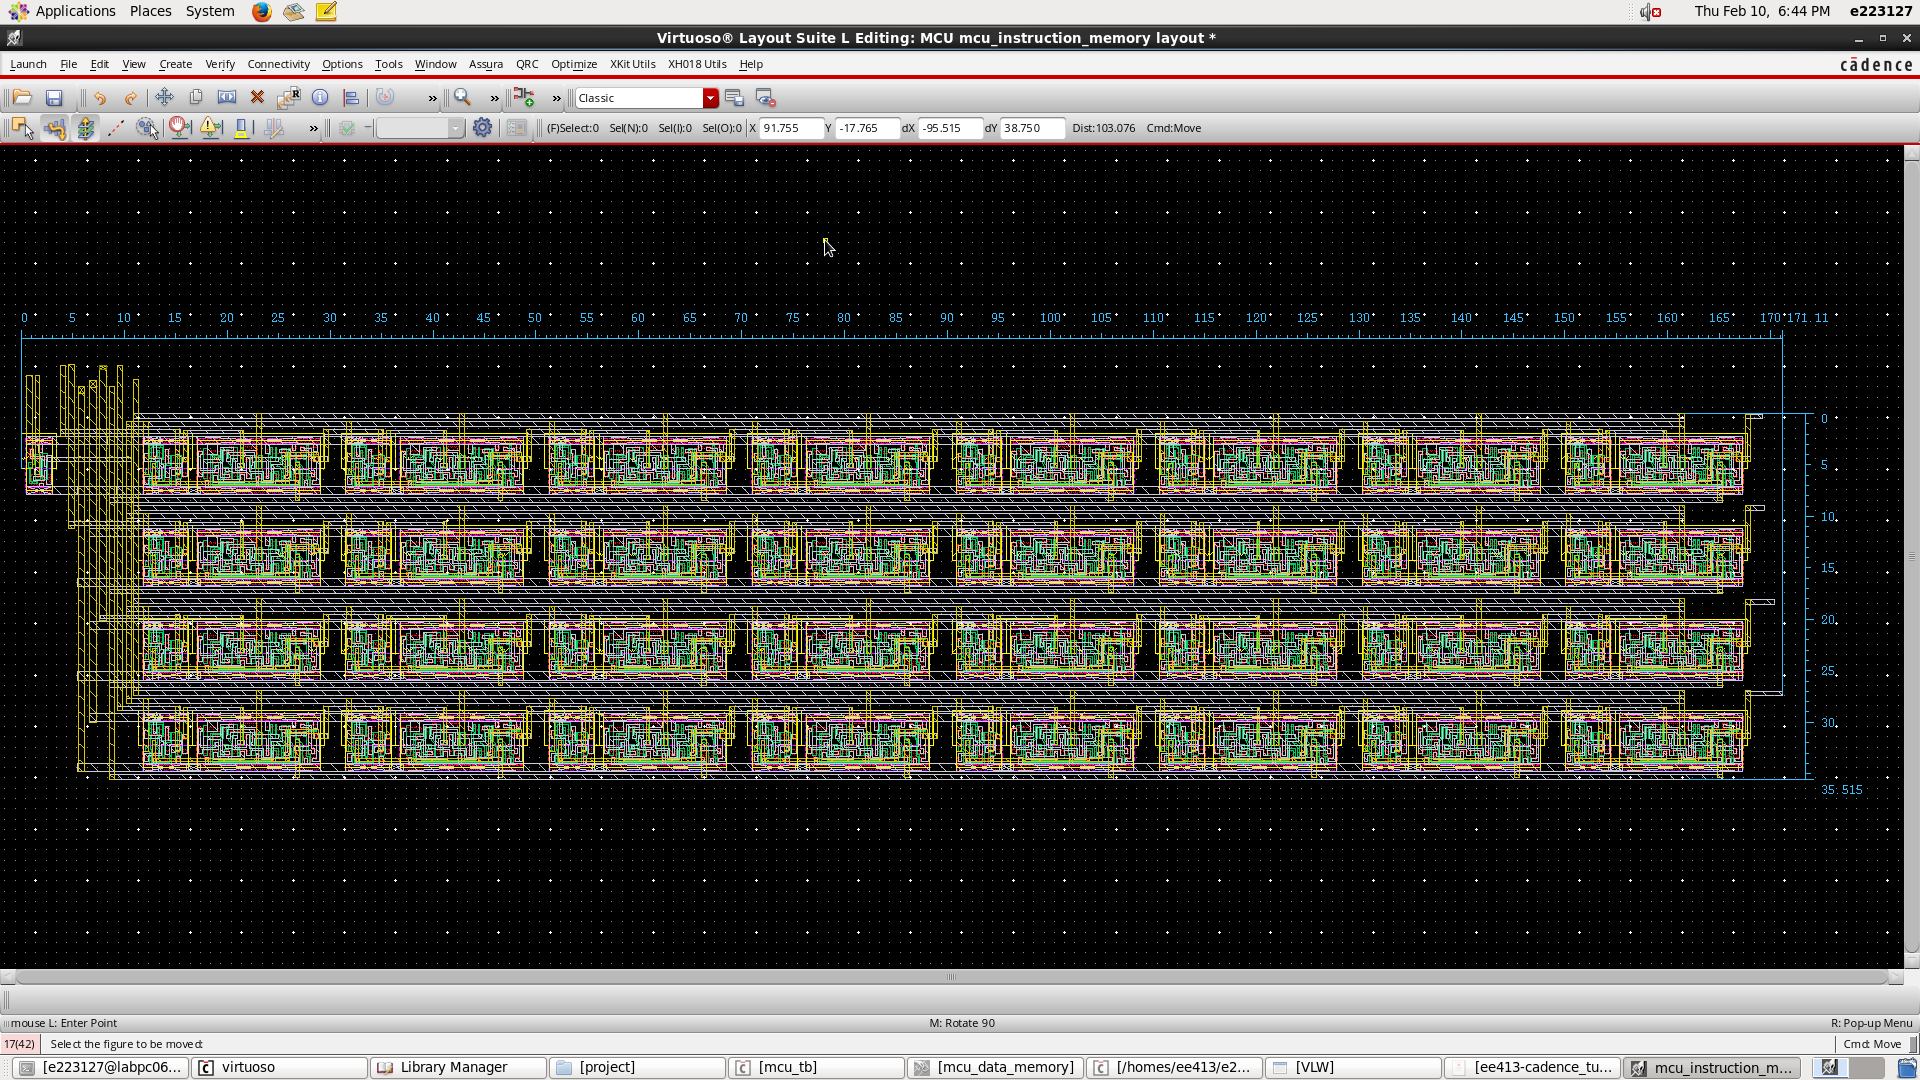
\includegraphics[scale=0.38]{instruction_layout.png}
\caption{Instruction Memory Layout}
\label{instruction_lay}
\end{figure}

\begin{figure}[H]
\centering
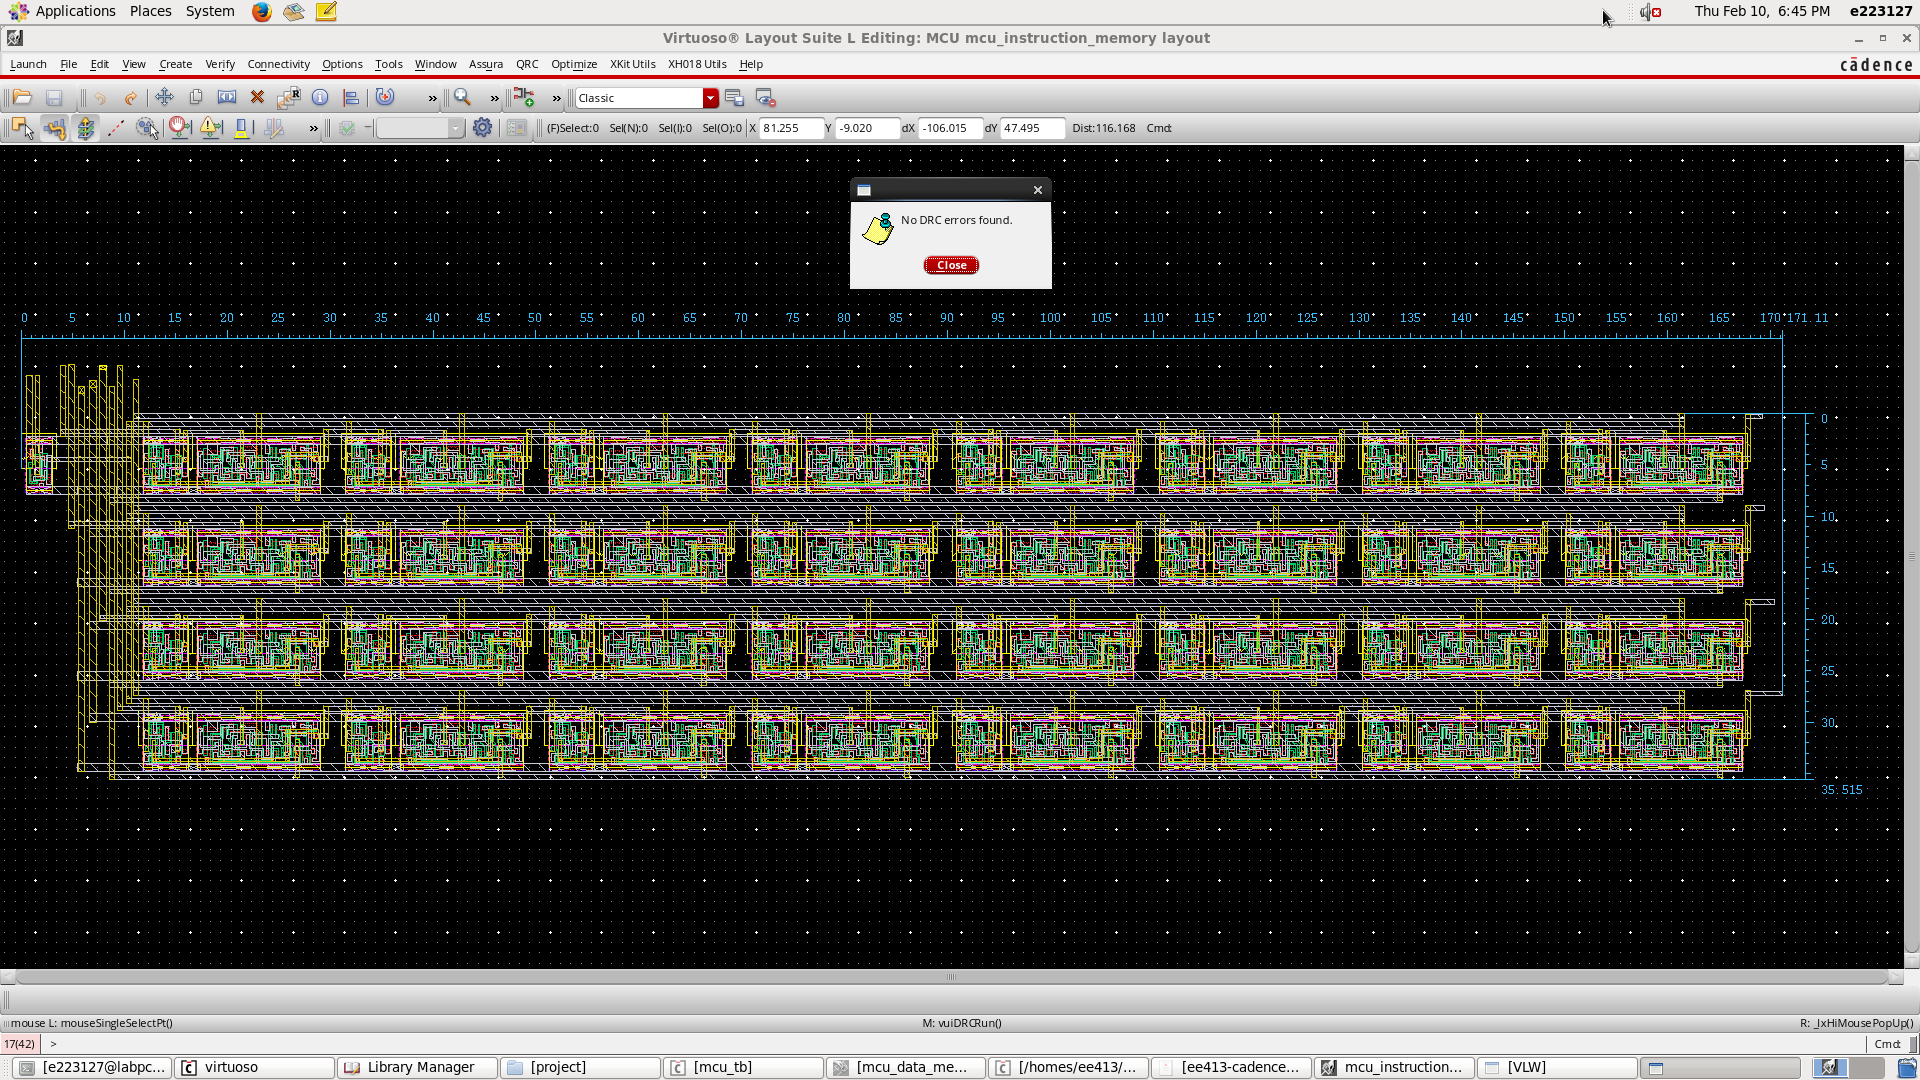
\includegraphics[scale=0.38]{instruction_drc.png}
\caption{Instruction Memory Layout DRC Result}
\label{instruction_drc}
\end{figure}


\begin{figure}[H]
\centering
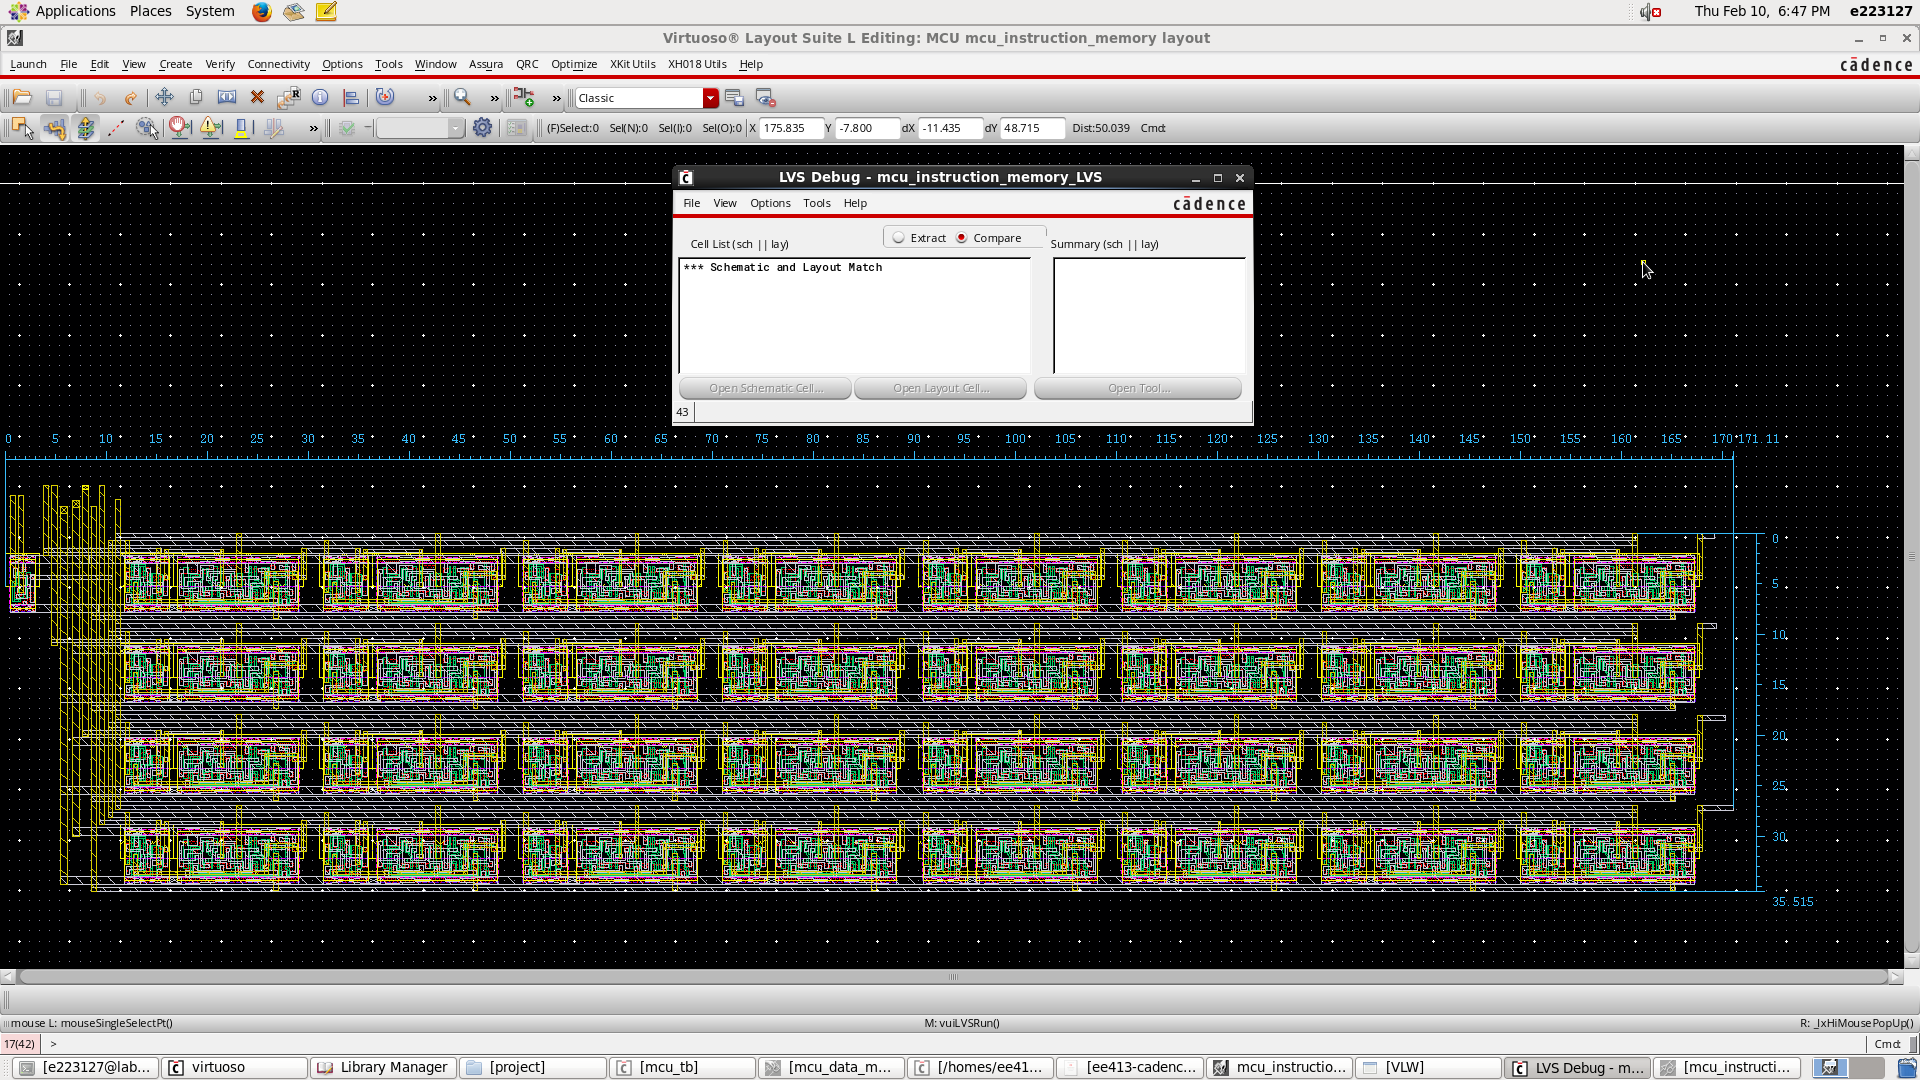
\includegraphics[scale=0.38]{instruction_lvs.png}
\caption{Instruction Memory Layout LVS Result}
\label{instruction_lvs}
\end{figure}

\begin{figure}[H]
\centering
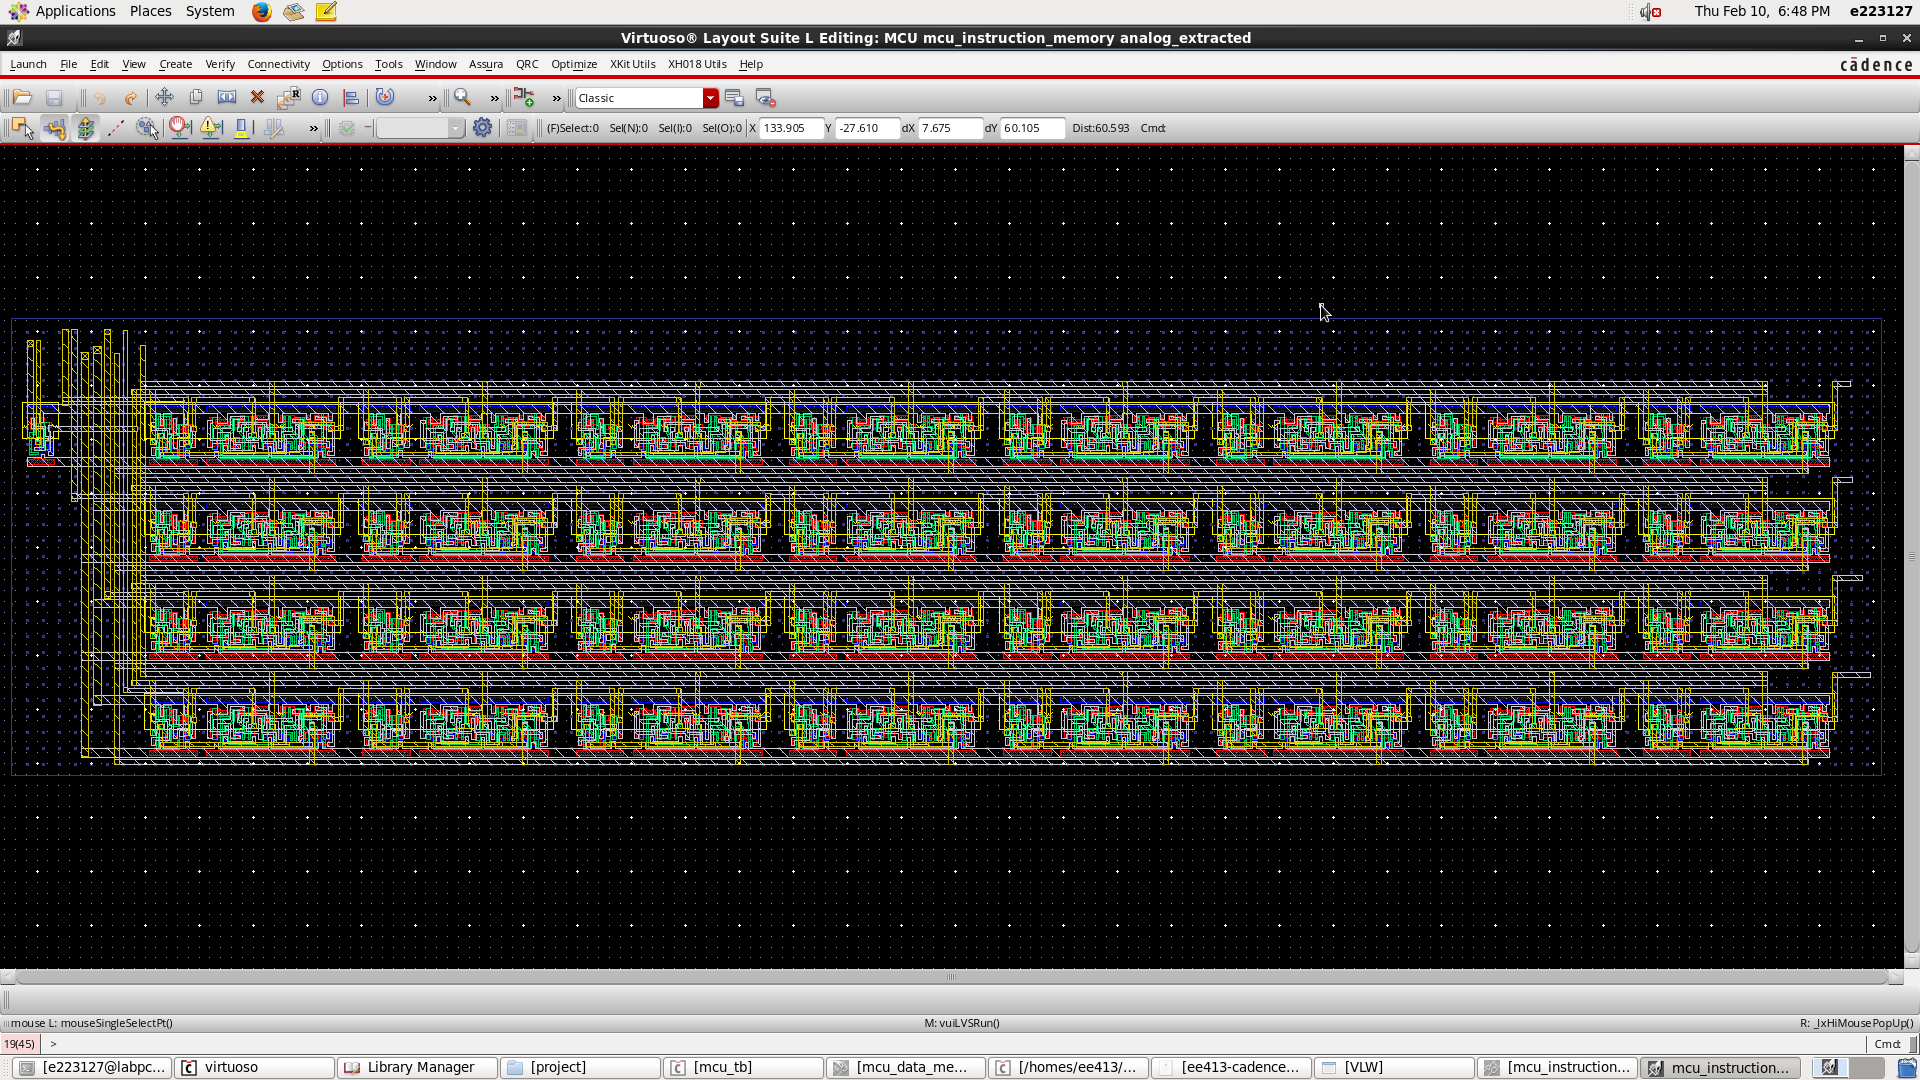
\includegraphics[scale=0.38]{instruction_extracted.png}
\caption{Instruction Memory Layout Parasitic Capacitance Extraction Result}
\label{instruction_extracted}
\end{figure}

\begin{figure}[H]
\centering
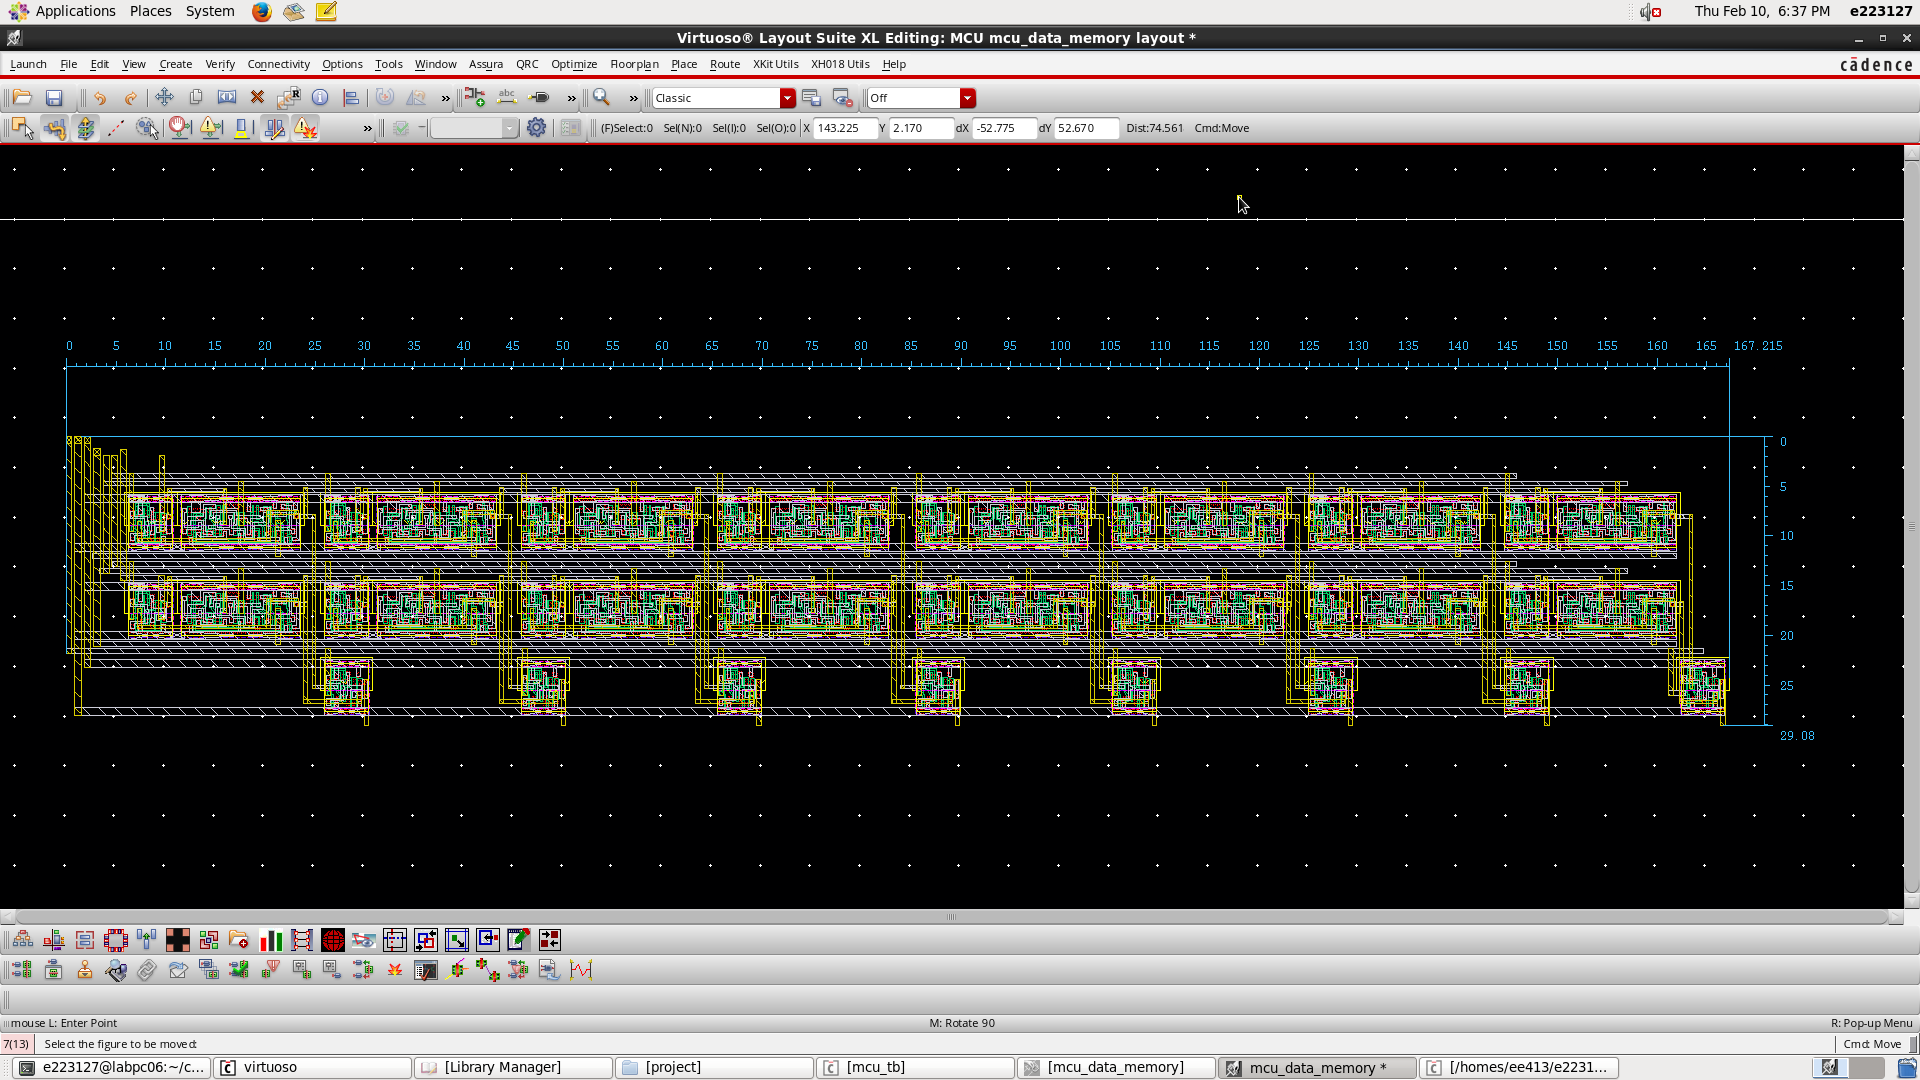
\includegraphics[scale=0.38]{data_layout.png}
\caption{Data Memory Layout}
\label{data_lay}
\end{figure}

\begin{figure}[H]
\centering
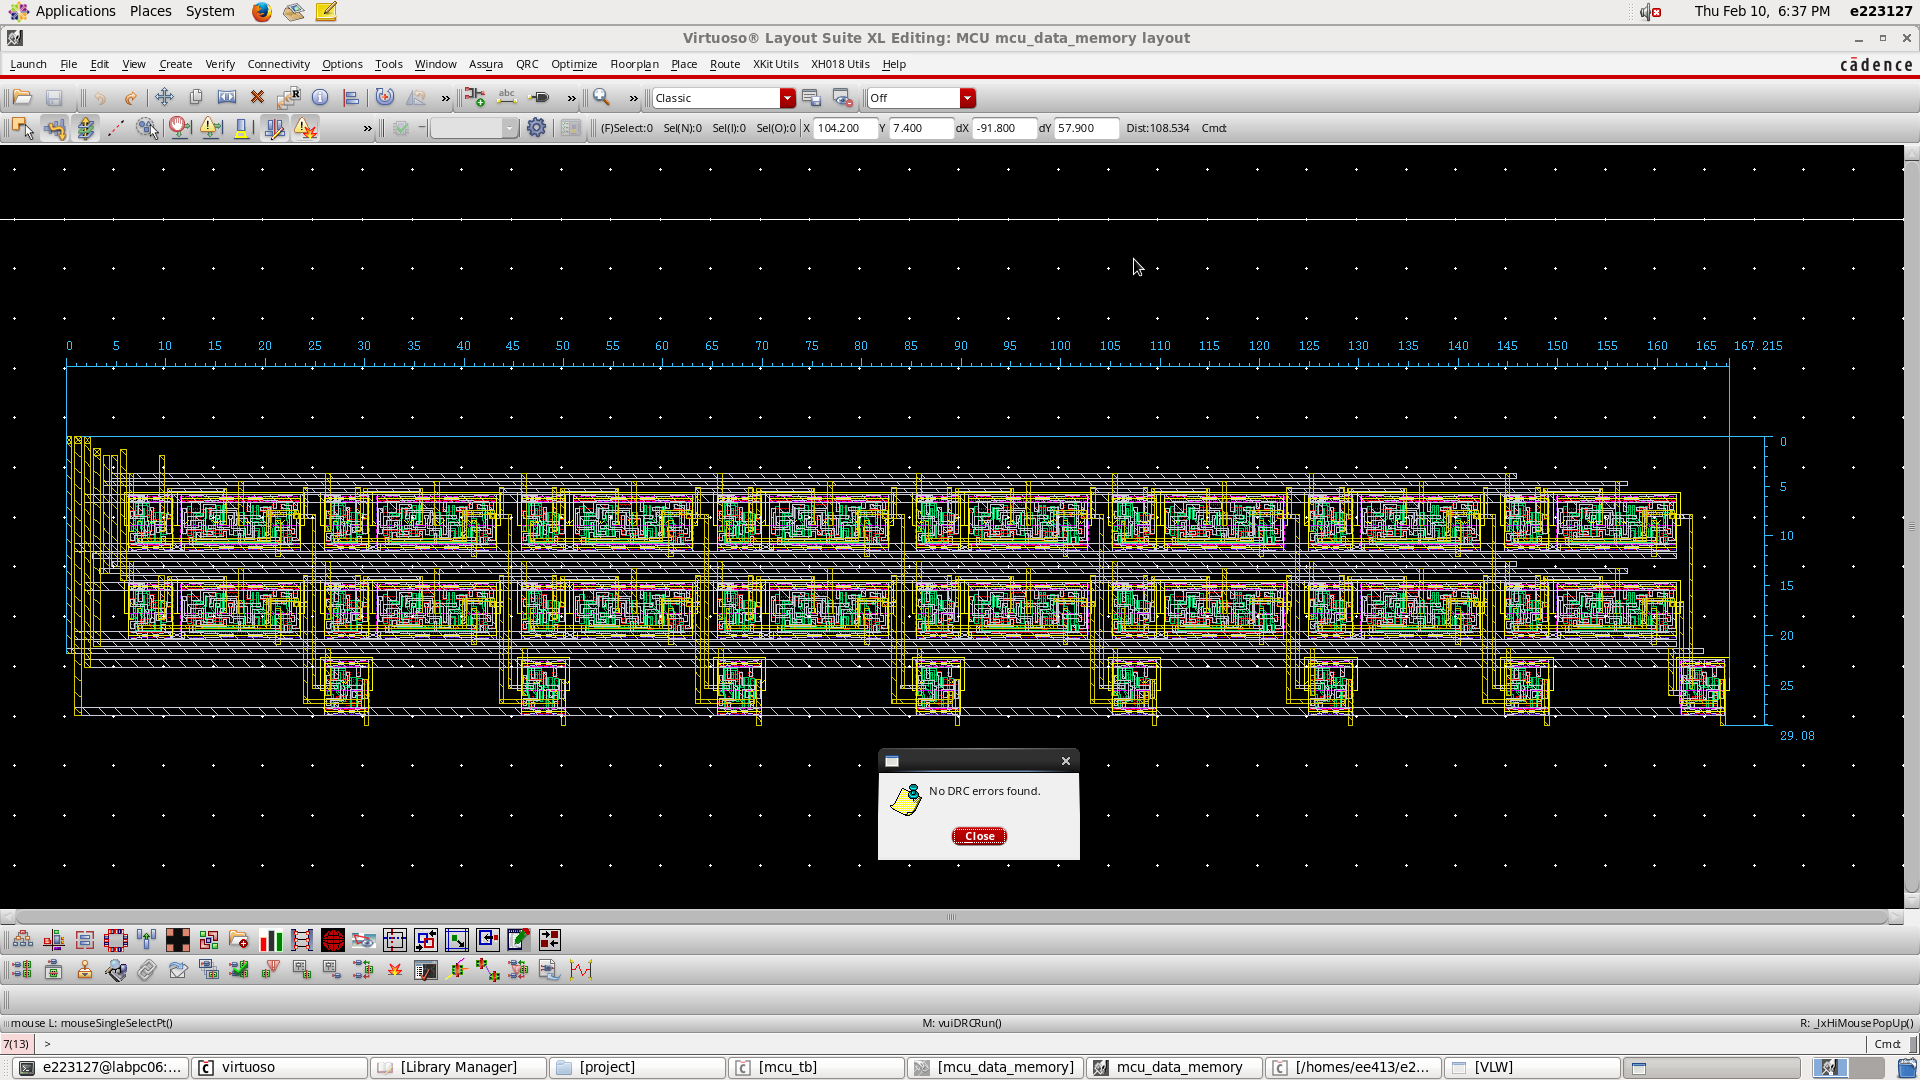
\includegraphics[scale=0.38]{data_drc.png}
\caption{Data Memory Layout DRC Result}
\label{data_drc}
\end{figure}


\begin{figure}[H]
\centering
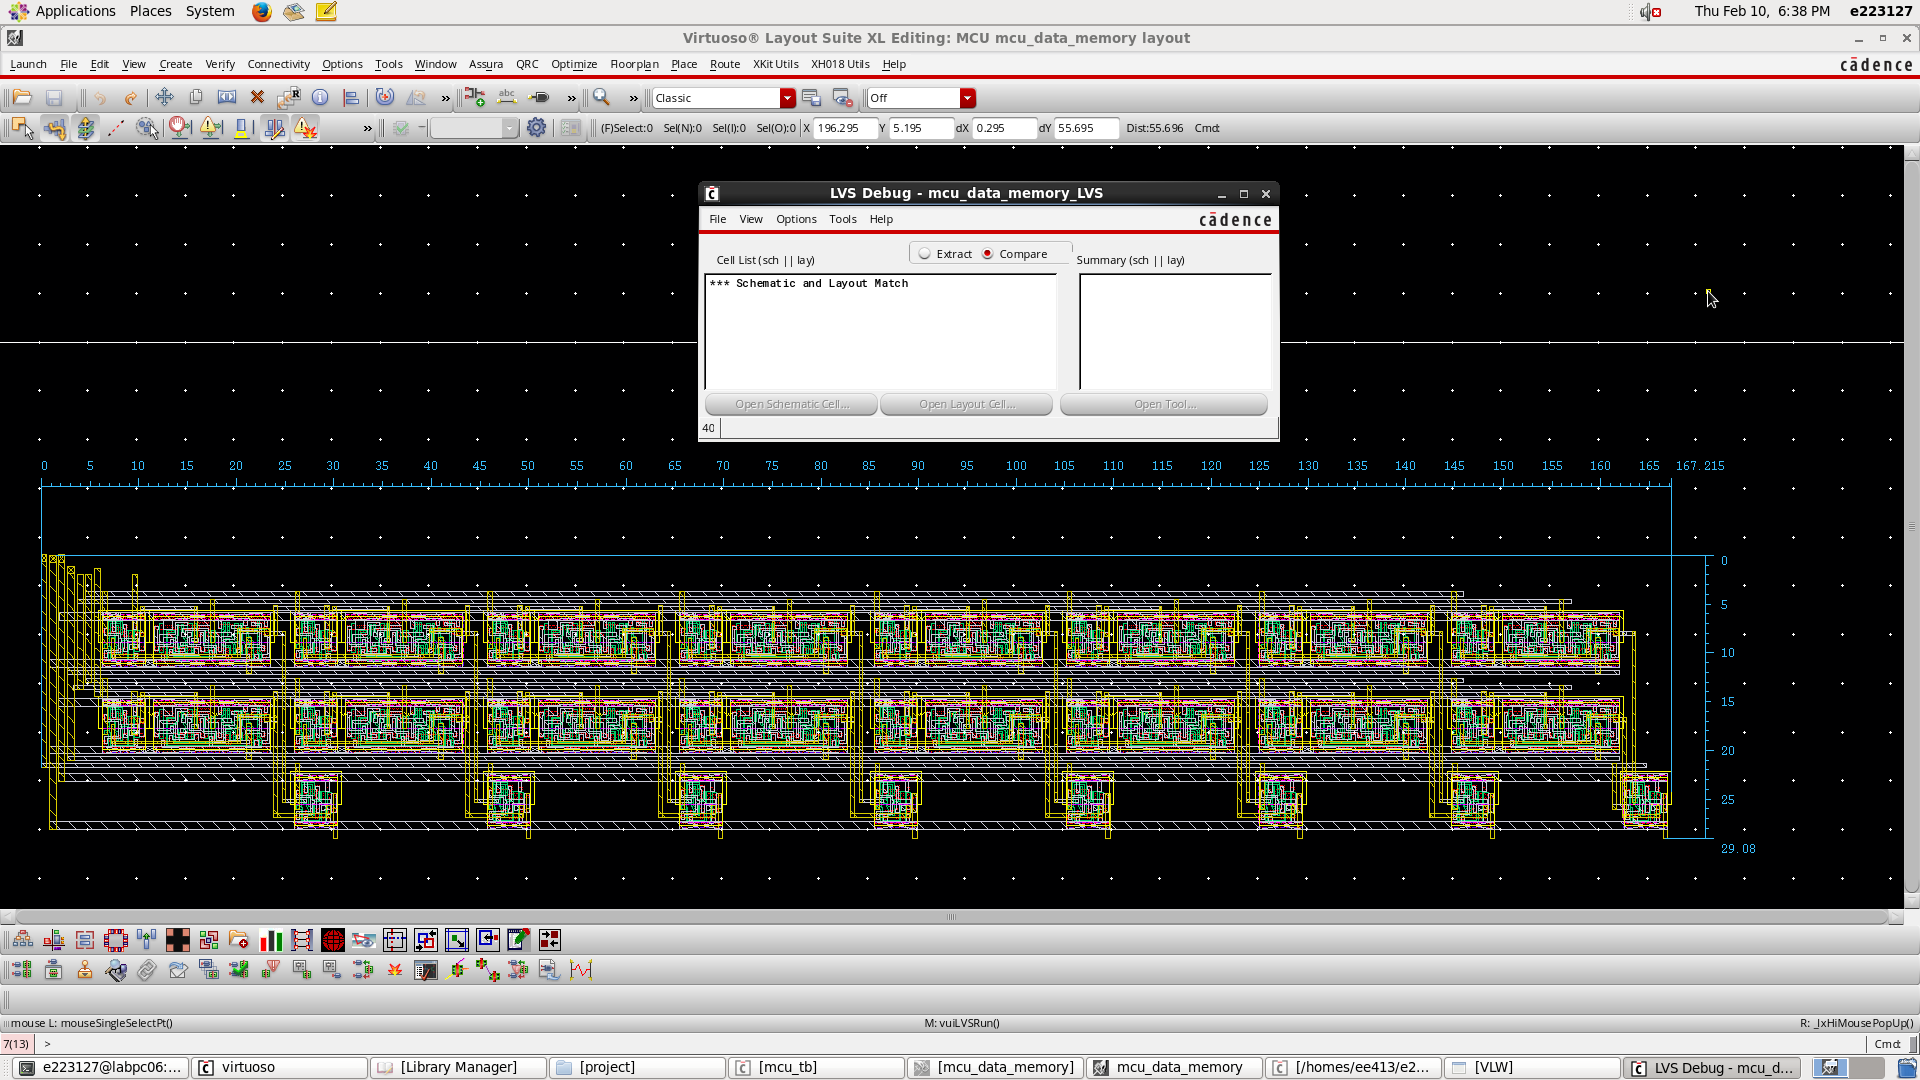
\includegraphics[scale=0.38]{data_lvs.png}
\caption{Data Memory Layout LVS Result}
\label{data_lvs}
\end{figure}

\begin{figure}[H]
\centering
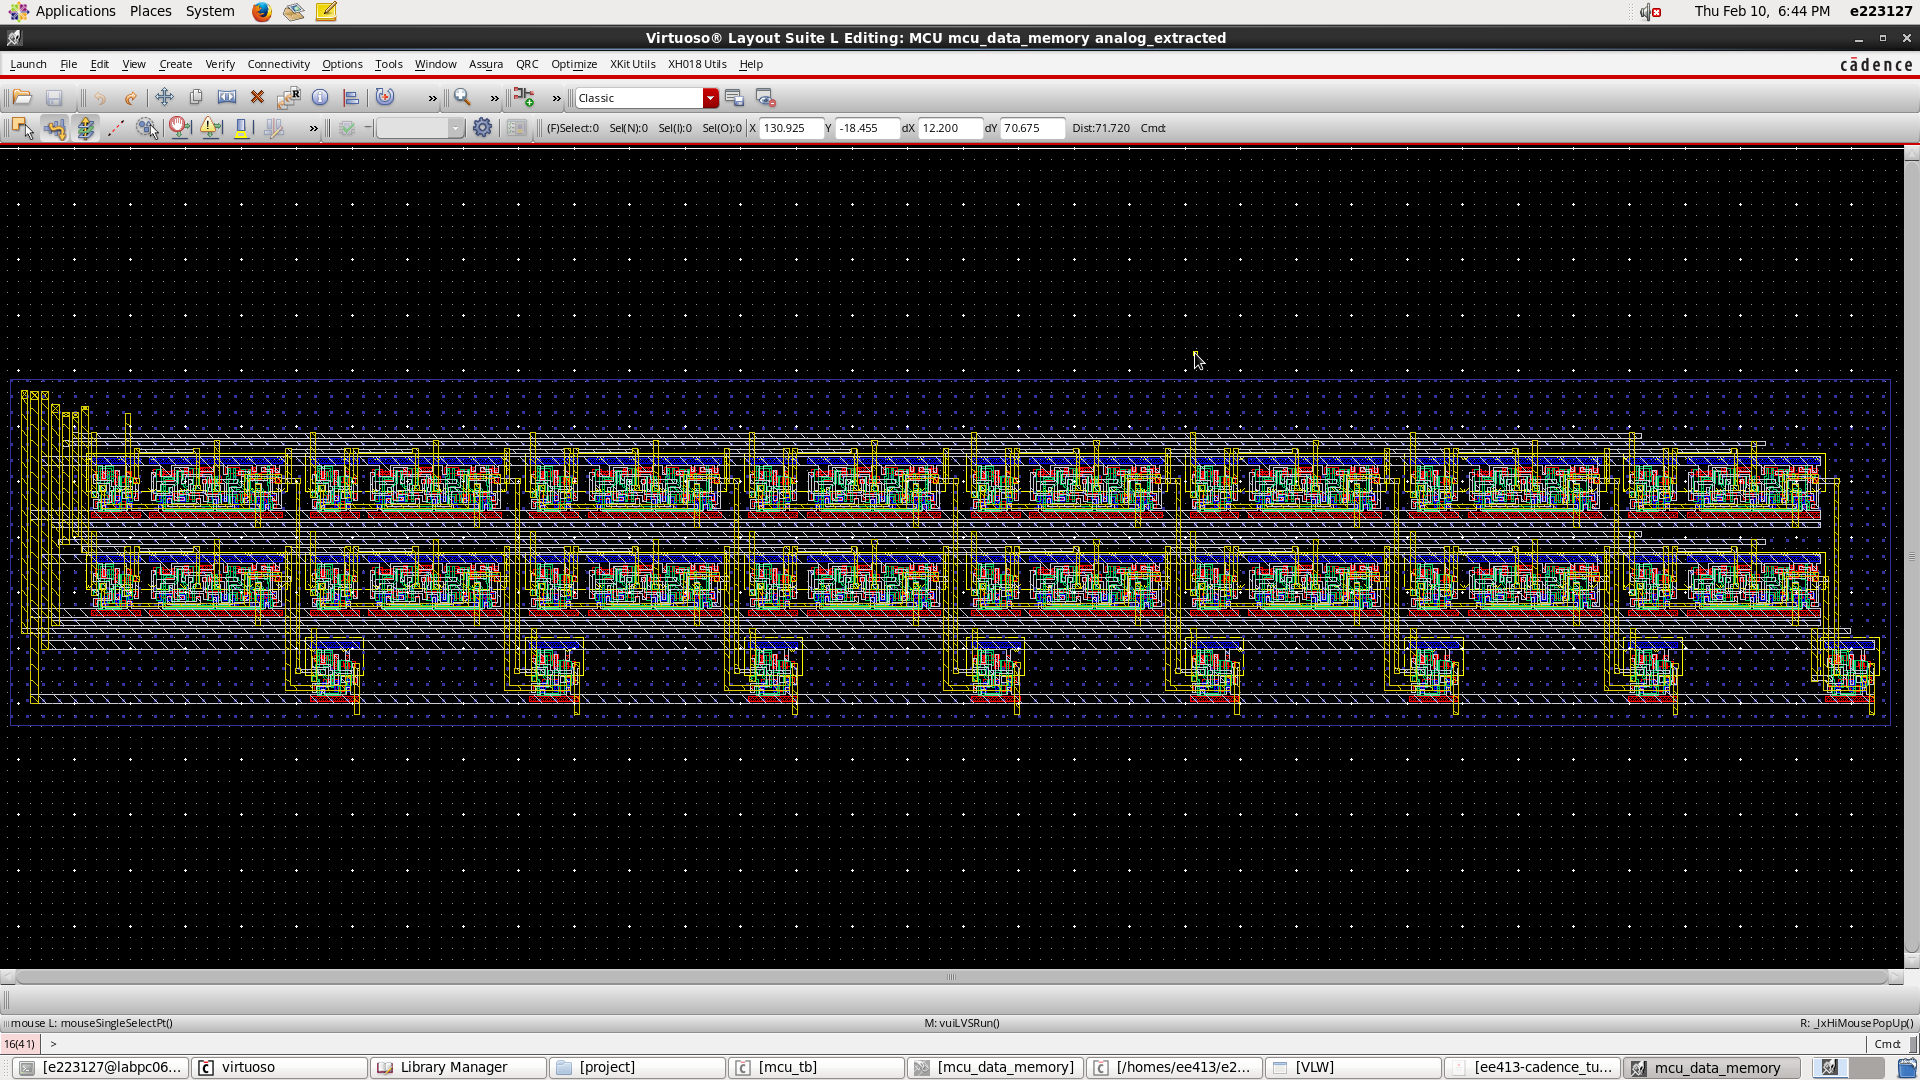
\includegraphics[scale=0.38]{data_extracted.png}
\caption{Data Memory Layout Parasitic Capacitance Extraction Result}
\label{data_extracted}
\end{figure}

\end{landscape}

\begin{landscape}

\pagestyle{empty}
\subsection*{Appendix}

\begin{figure}[H]
\centering
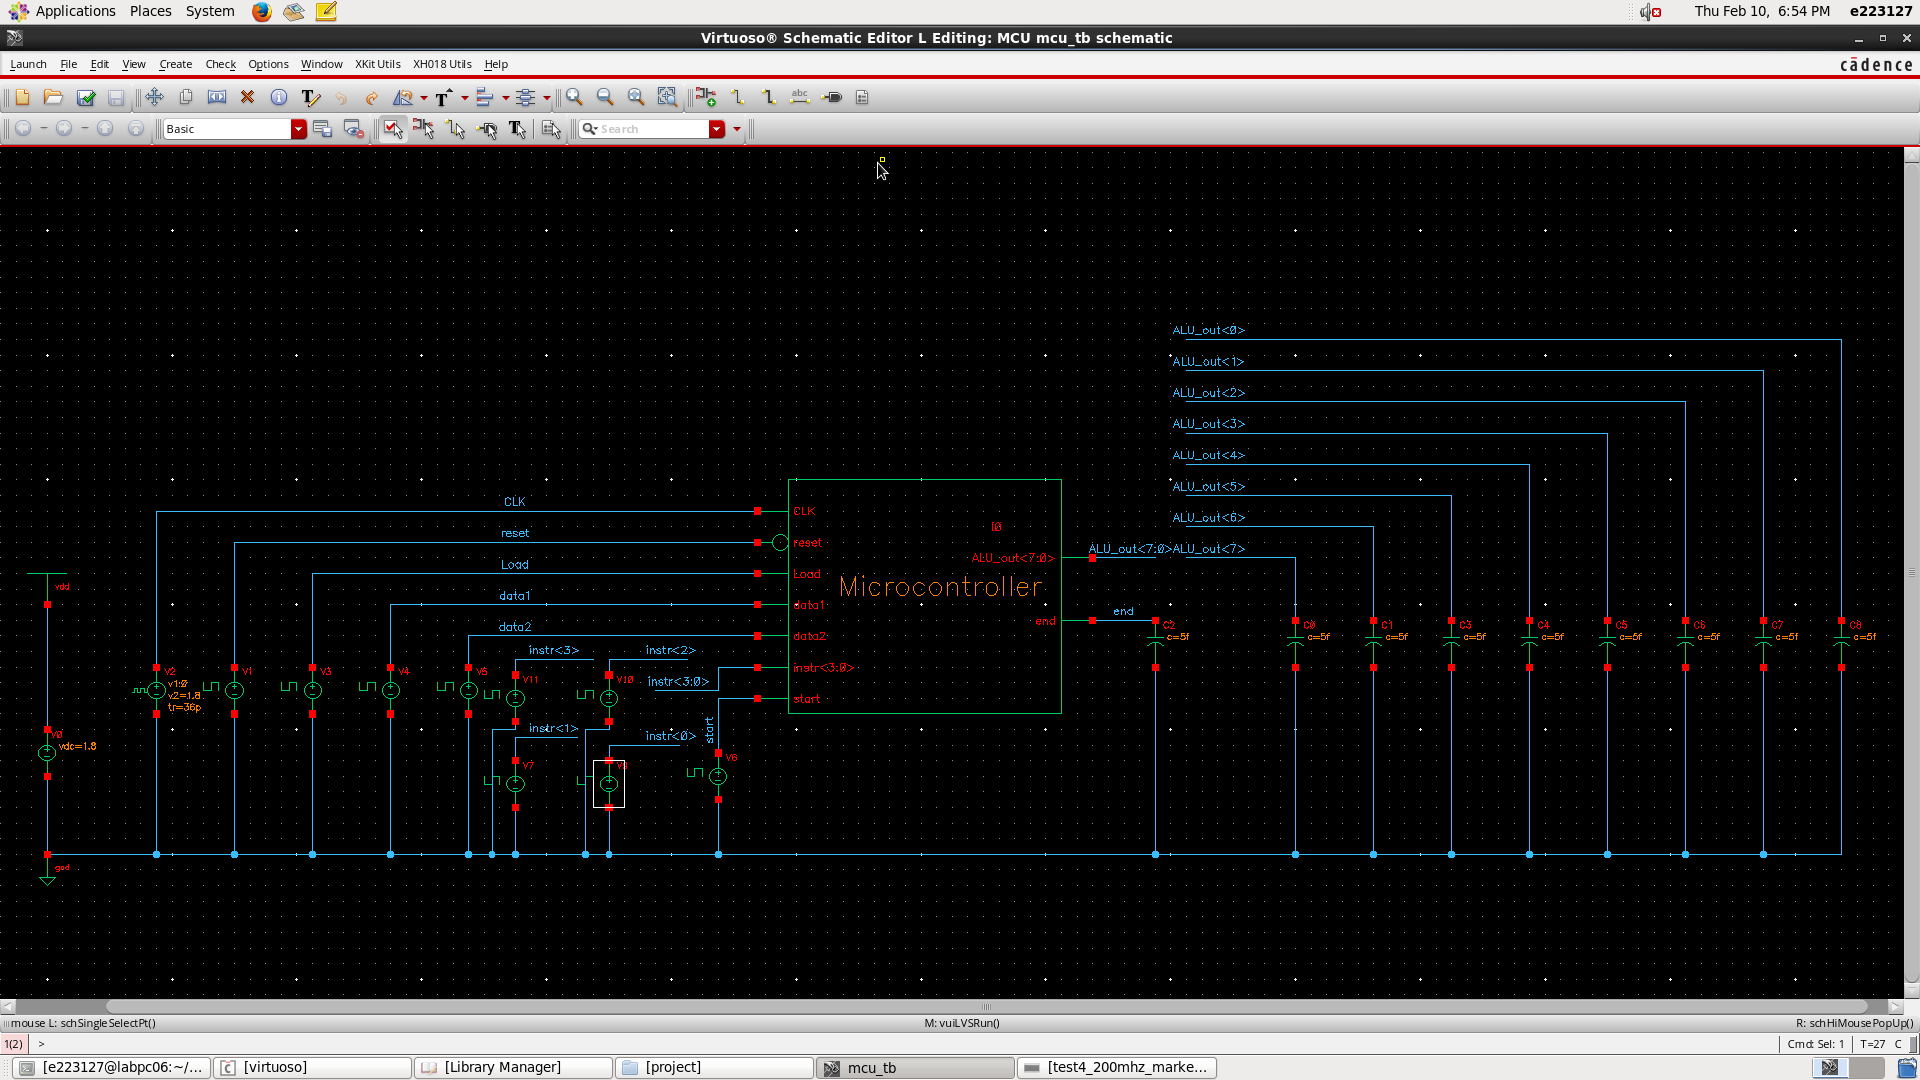
\includegraphics[scale=0.38]{testbench.png}
\caption{Testbench Schematic}
\label{tb}
\end{figure}


\begin{figure}[H]
\centering
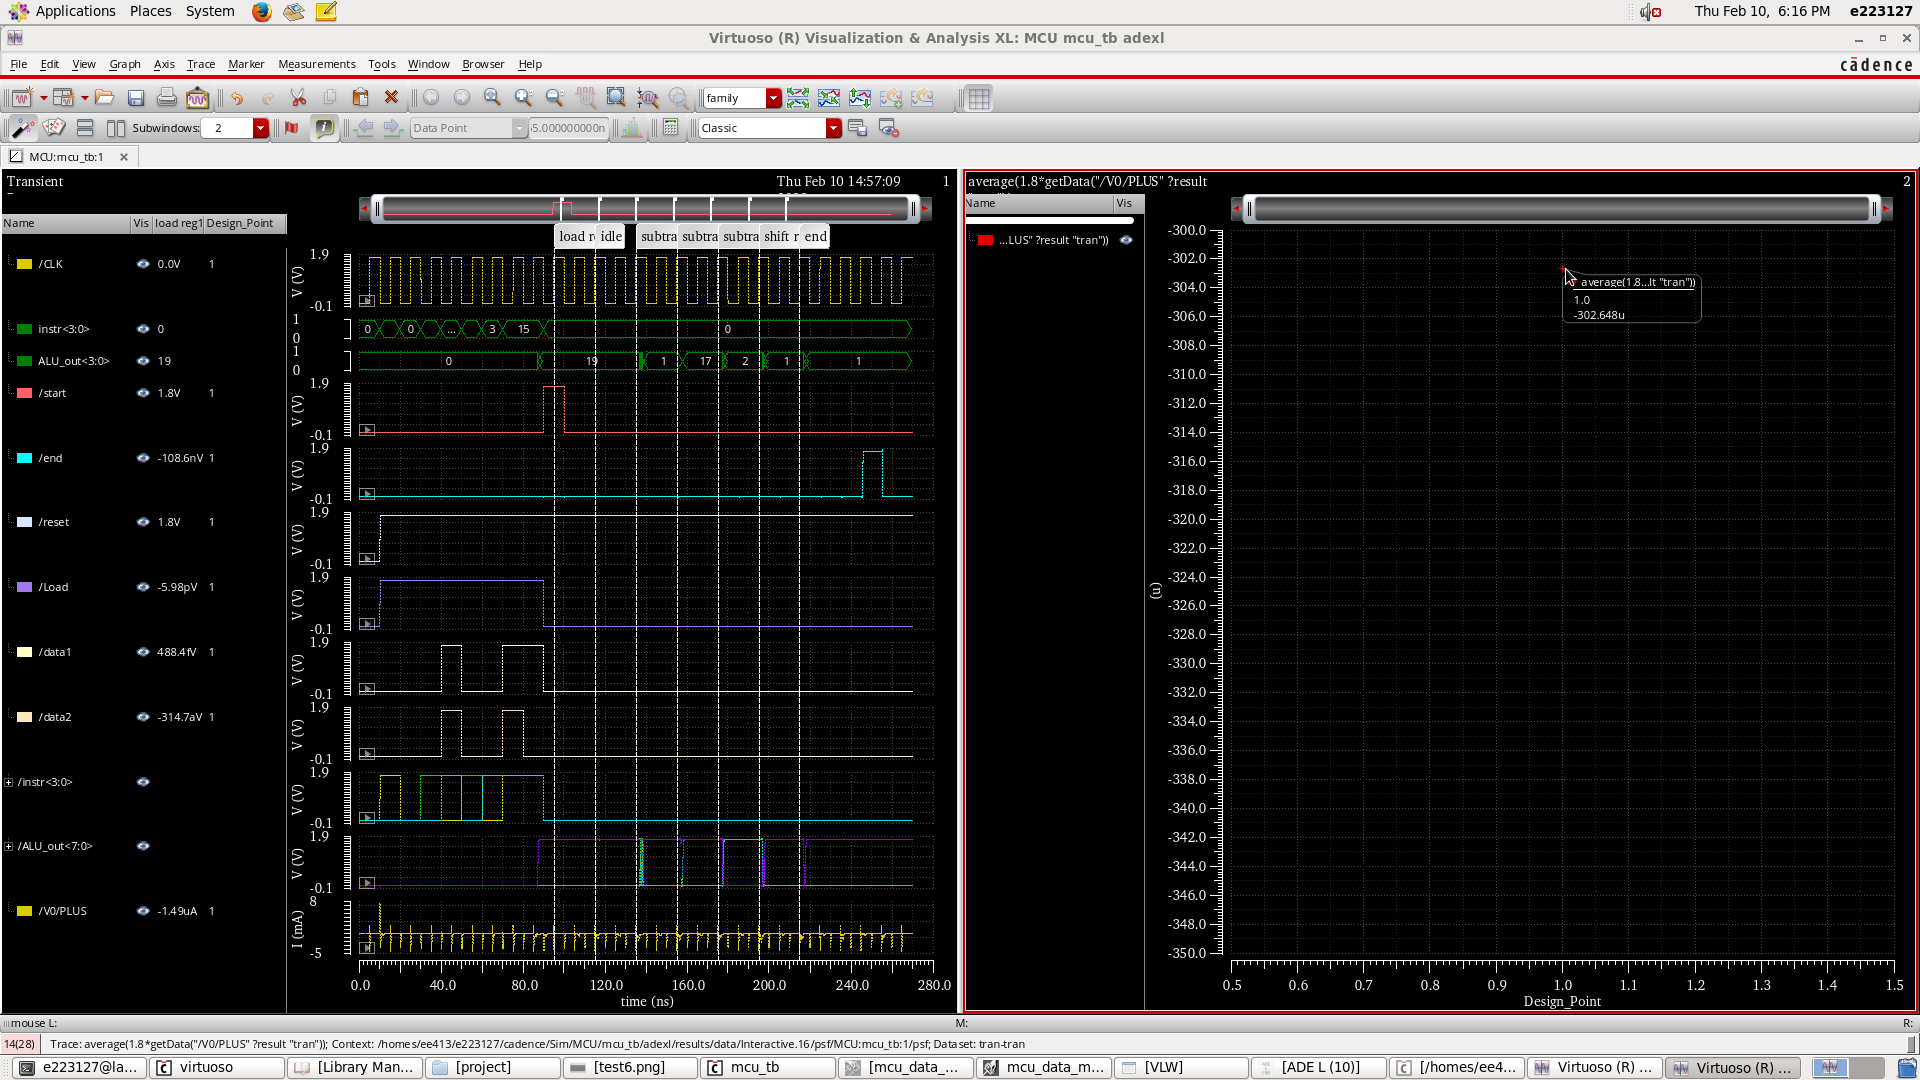
\includegraphics[scale=0.38]{test6_power.png}
\caption{Test-1 Power Dissipation Result}
\label{test6_power}
\end{figure}



\begin{figure}[H]
\centering
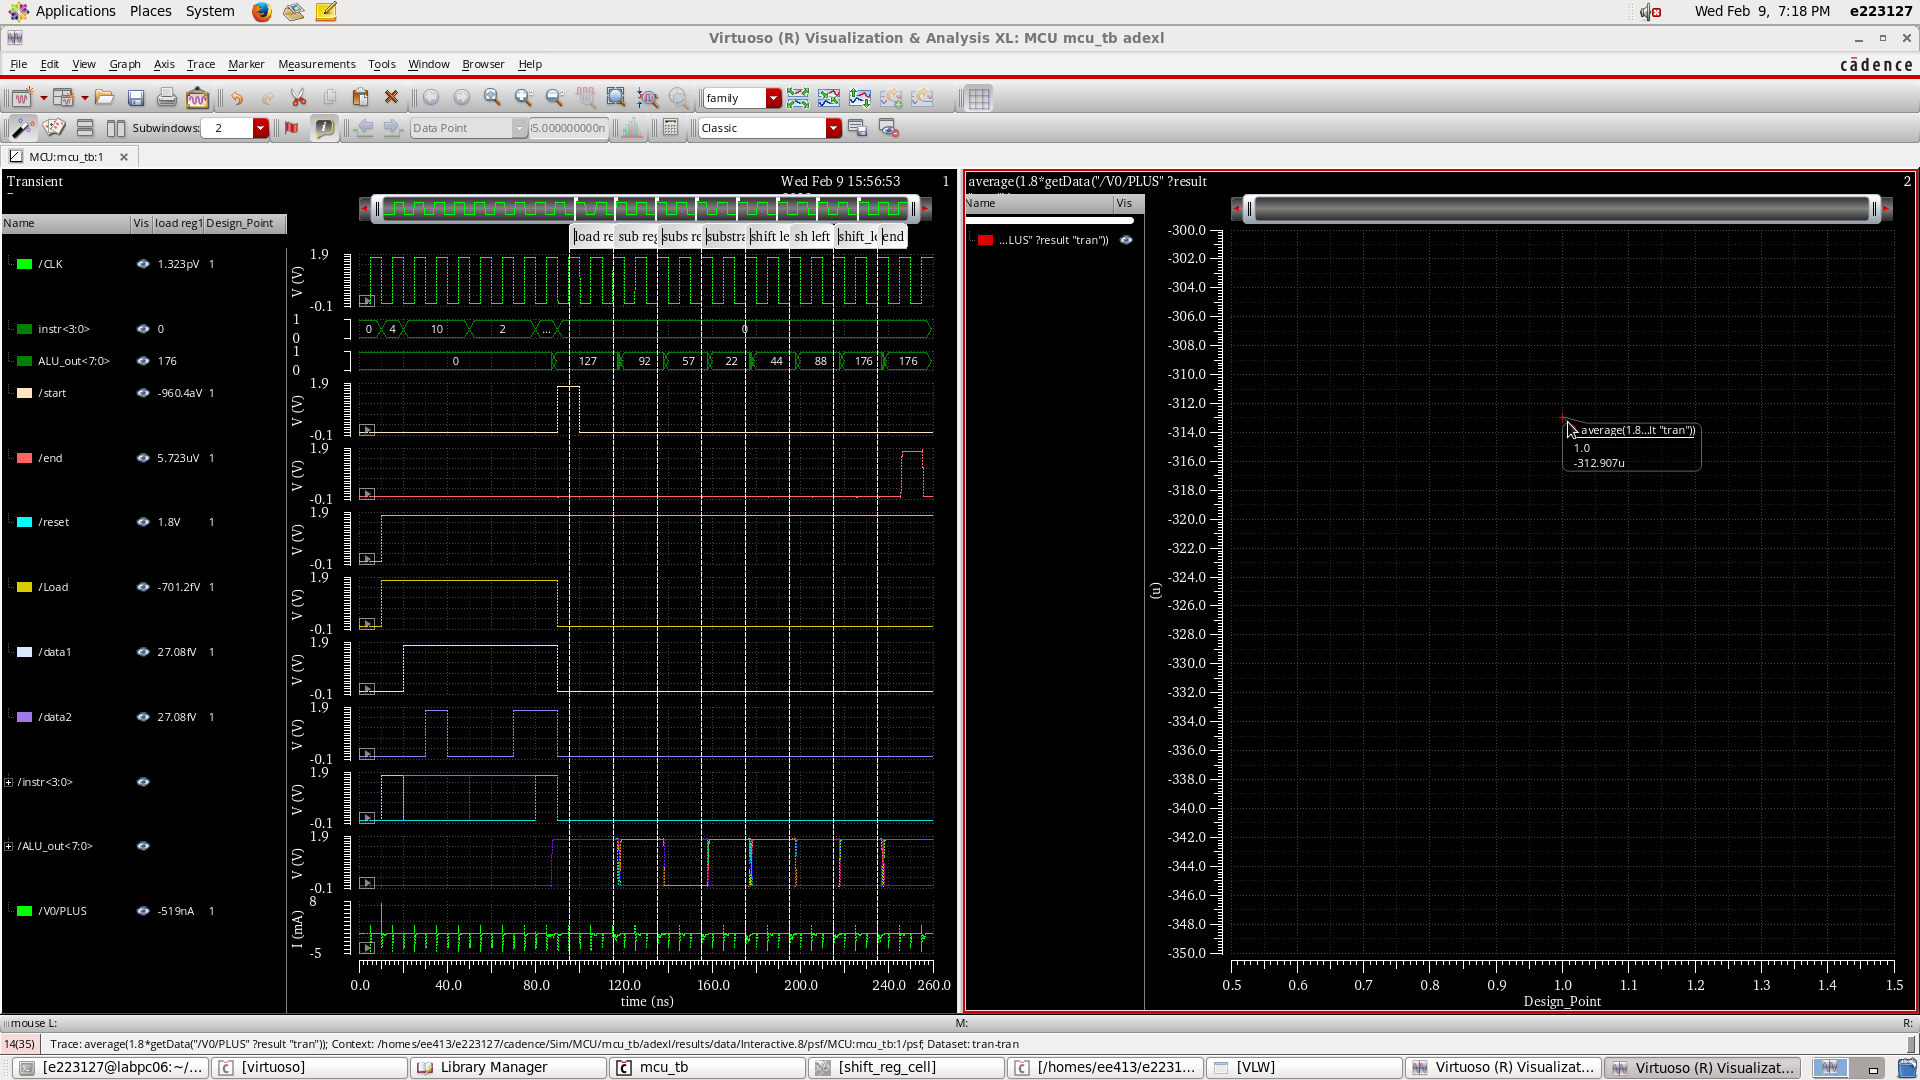
\includegraphics[scale=0.38]{test1_power_100mhz.png}
\caption{Test-2 Power Dissipation Result}
\label{test1_power}
\end{figure}


\begin{figure}[H]
\centering
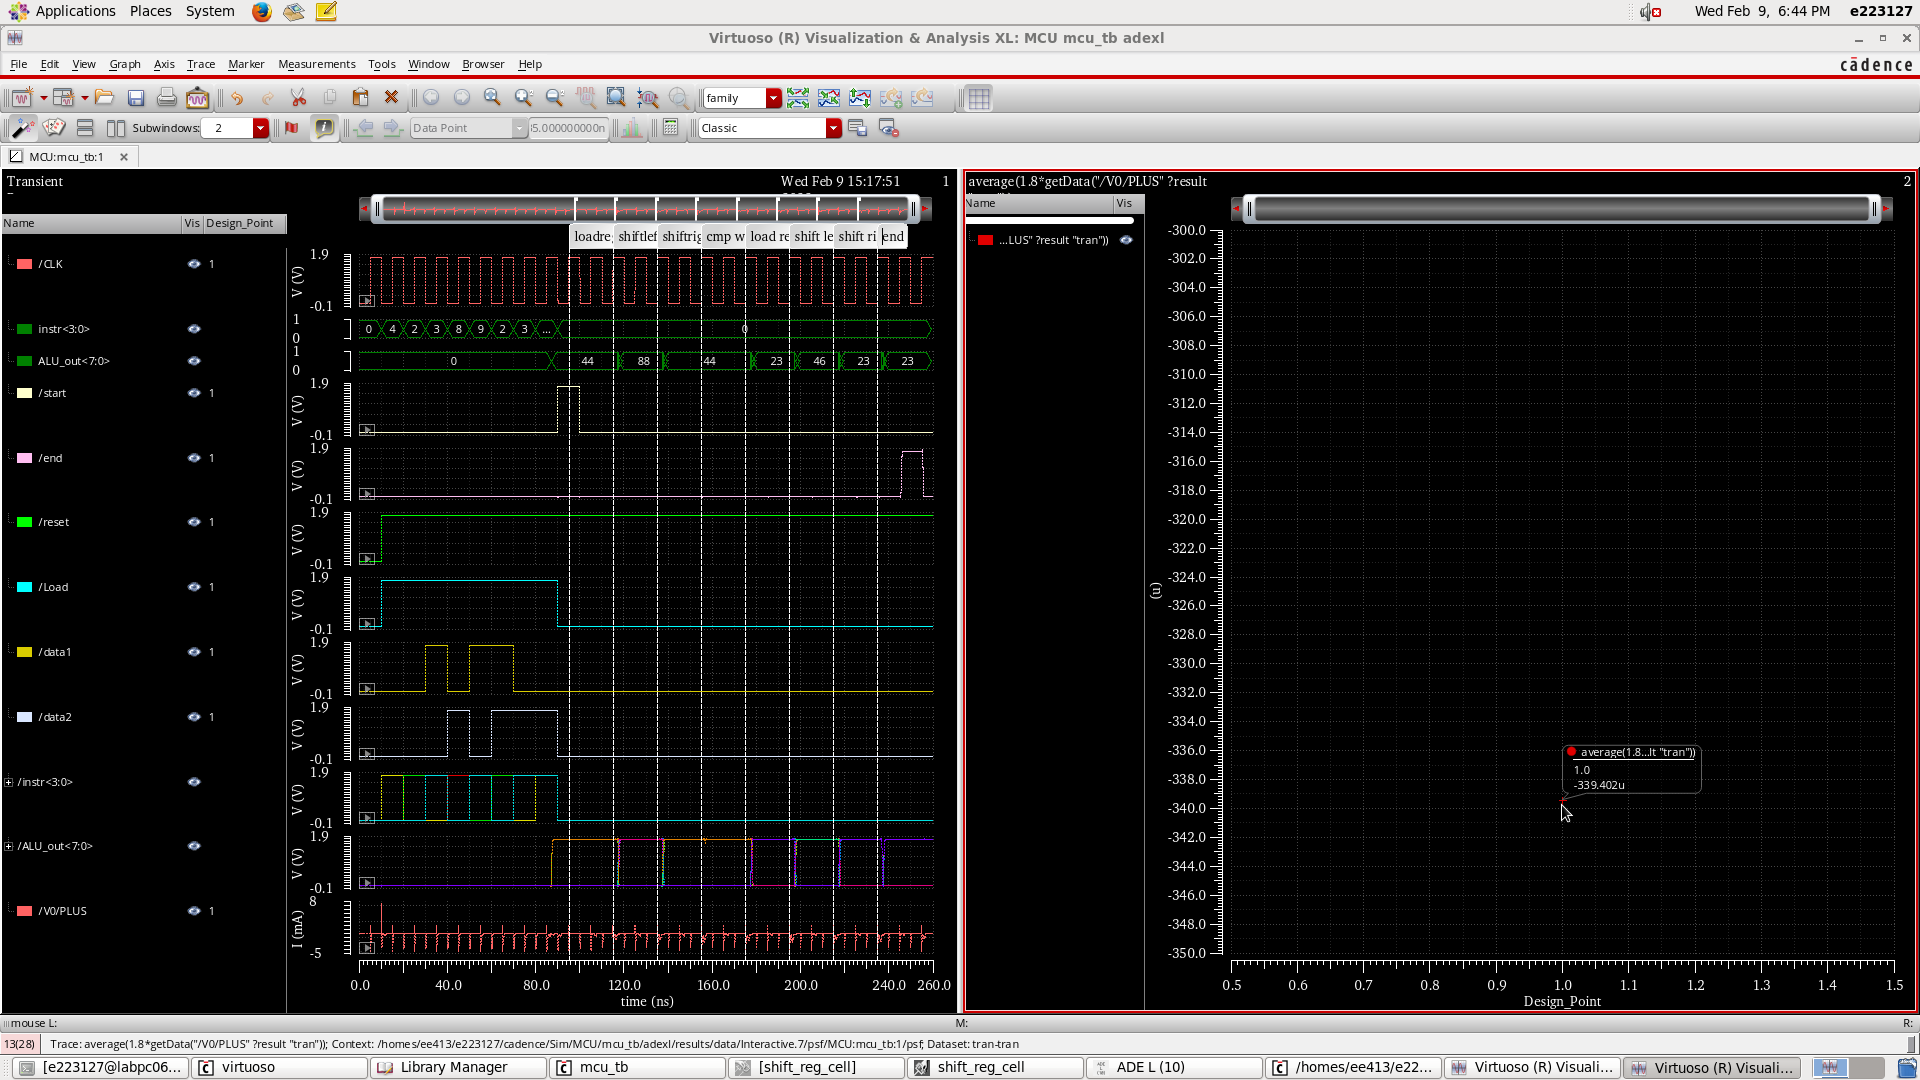
\includegraphics[scale=0.38]{test2_power.png}
\caption{Test-3 Power Dissipation Result}
\label{test2_power}
\end{figure}



\begin{figure}[H]
\centering
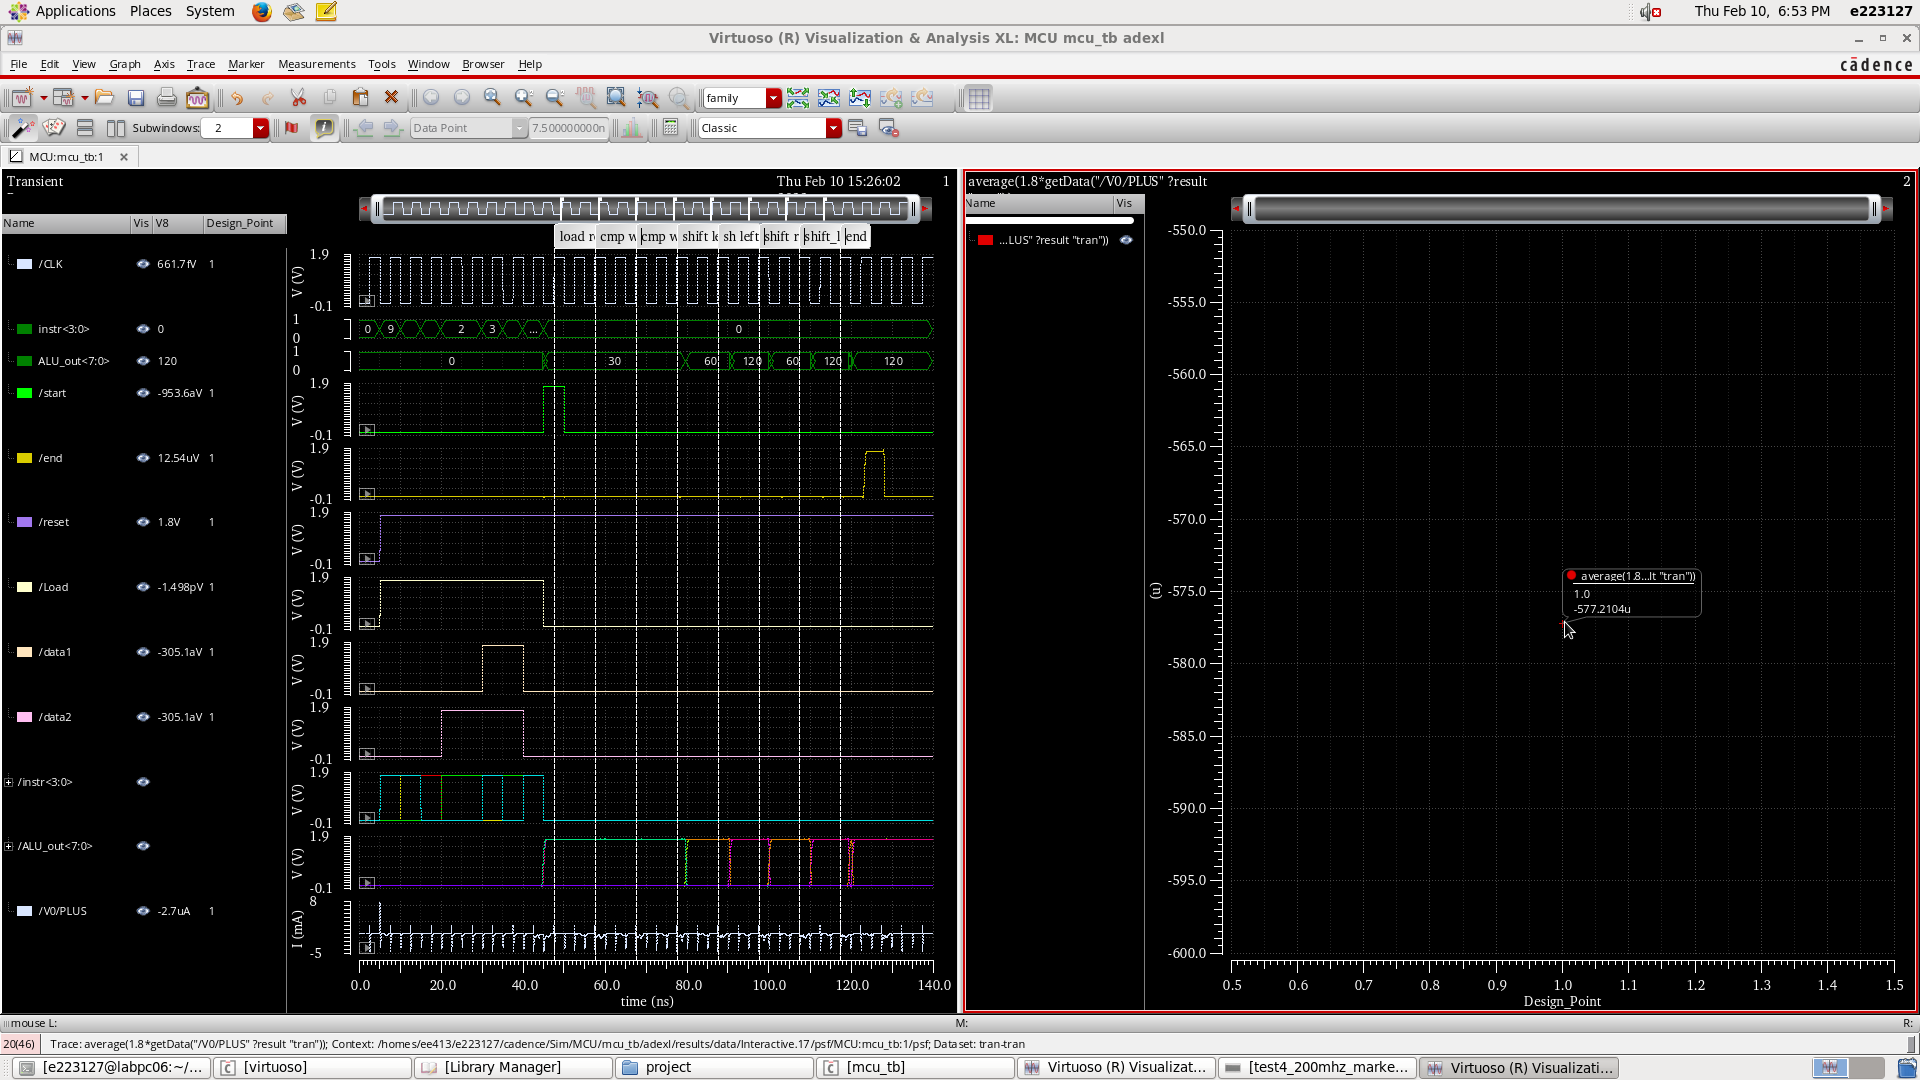
\includegraphics[scale=0.38]{test4_power.png}
\caption{Test-4 Power Dissipation Result}
\label{test4_power}
\end{figure}

\begin{figure}[H]
\centering
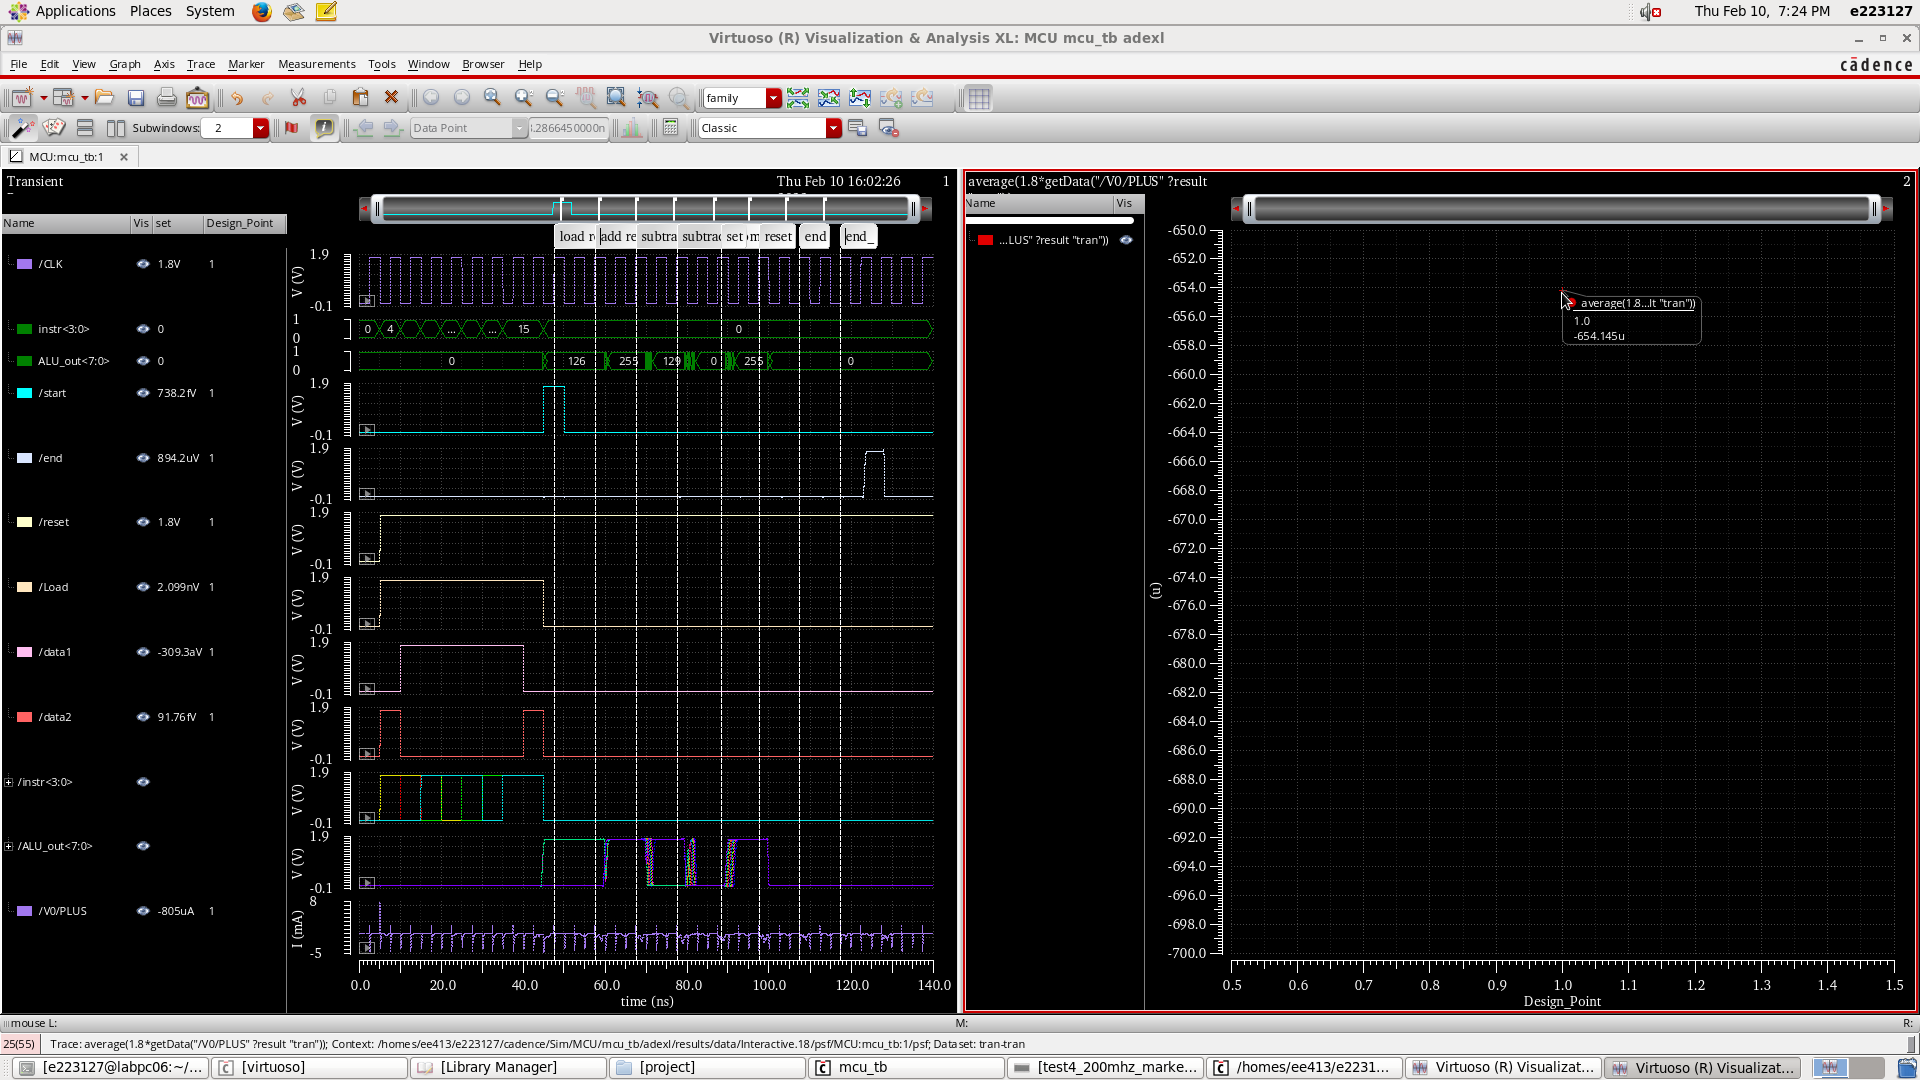
\includegraphics[scale=0.38]{test3_200mhz_power.png}
\caption{Test-5 Power Dissipation Result}
\label{test3_power}
\end{figure}


\end{landscape}

\end{document}
